\section{Reference figures}

\subsection{From sections \ref{sec:reverification} and \ref{sec:finalCharacterization}}
\subsubsection{Focal-plane measurement figures}

One of two common plots from sections \ref{sec:reverification} and \ref{sec:finalCharacterization} is a focal-plane measurement plot, showing eo-pipe measurements in different runs. These plots are constructed to show measurements arranged localized to the LSSTCam focal plane orientation. Different sensors are plotted in different colors, with one point plotted for each amplifier on each sensor. The plots are arranged such that an apples-to-apples comparison is made between two different runs (see figure \ref{fig:ref:eoPipeFP_5x5}). On one axis is the measurements from one run, while the other axis has the measurements from a different run. If the measurements are consistent, the points should fall along the identity line. Deviations from measurements on the identity line indicate that one run is measuring the quantity at a higher or lower value than the other run. This plot is useful for identifying localized deviations between different runs, and also e2v and ITL specific behavior.

\begin{figure}
    \centering
    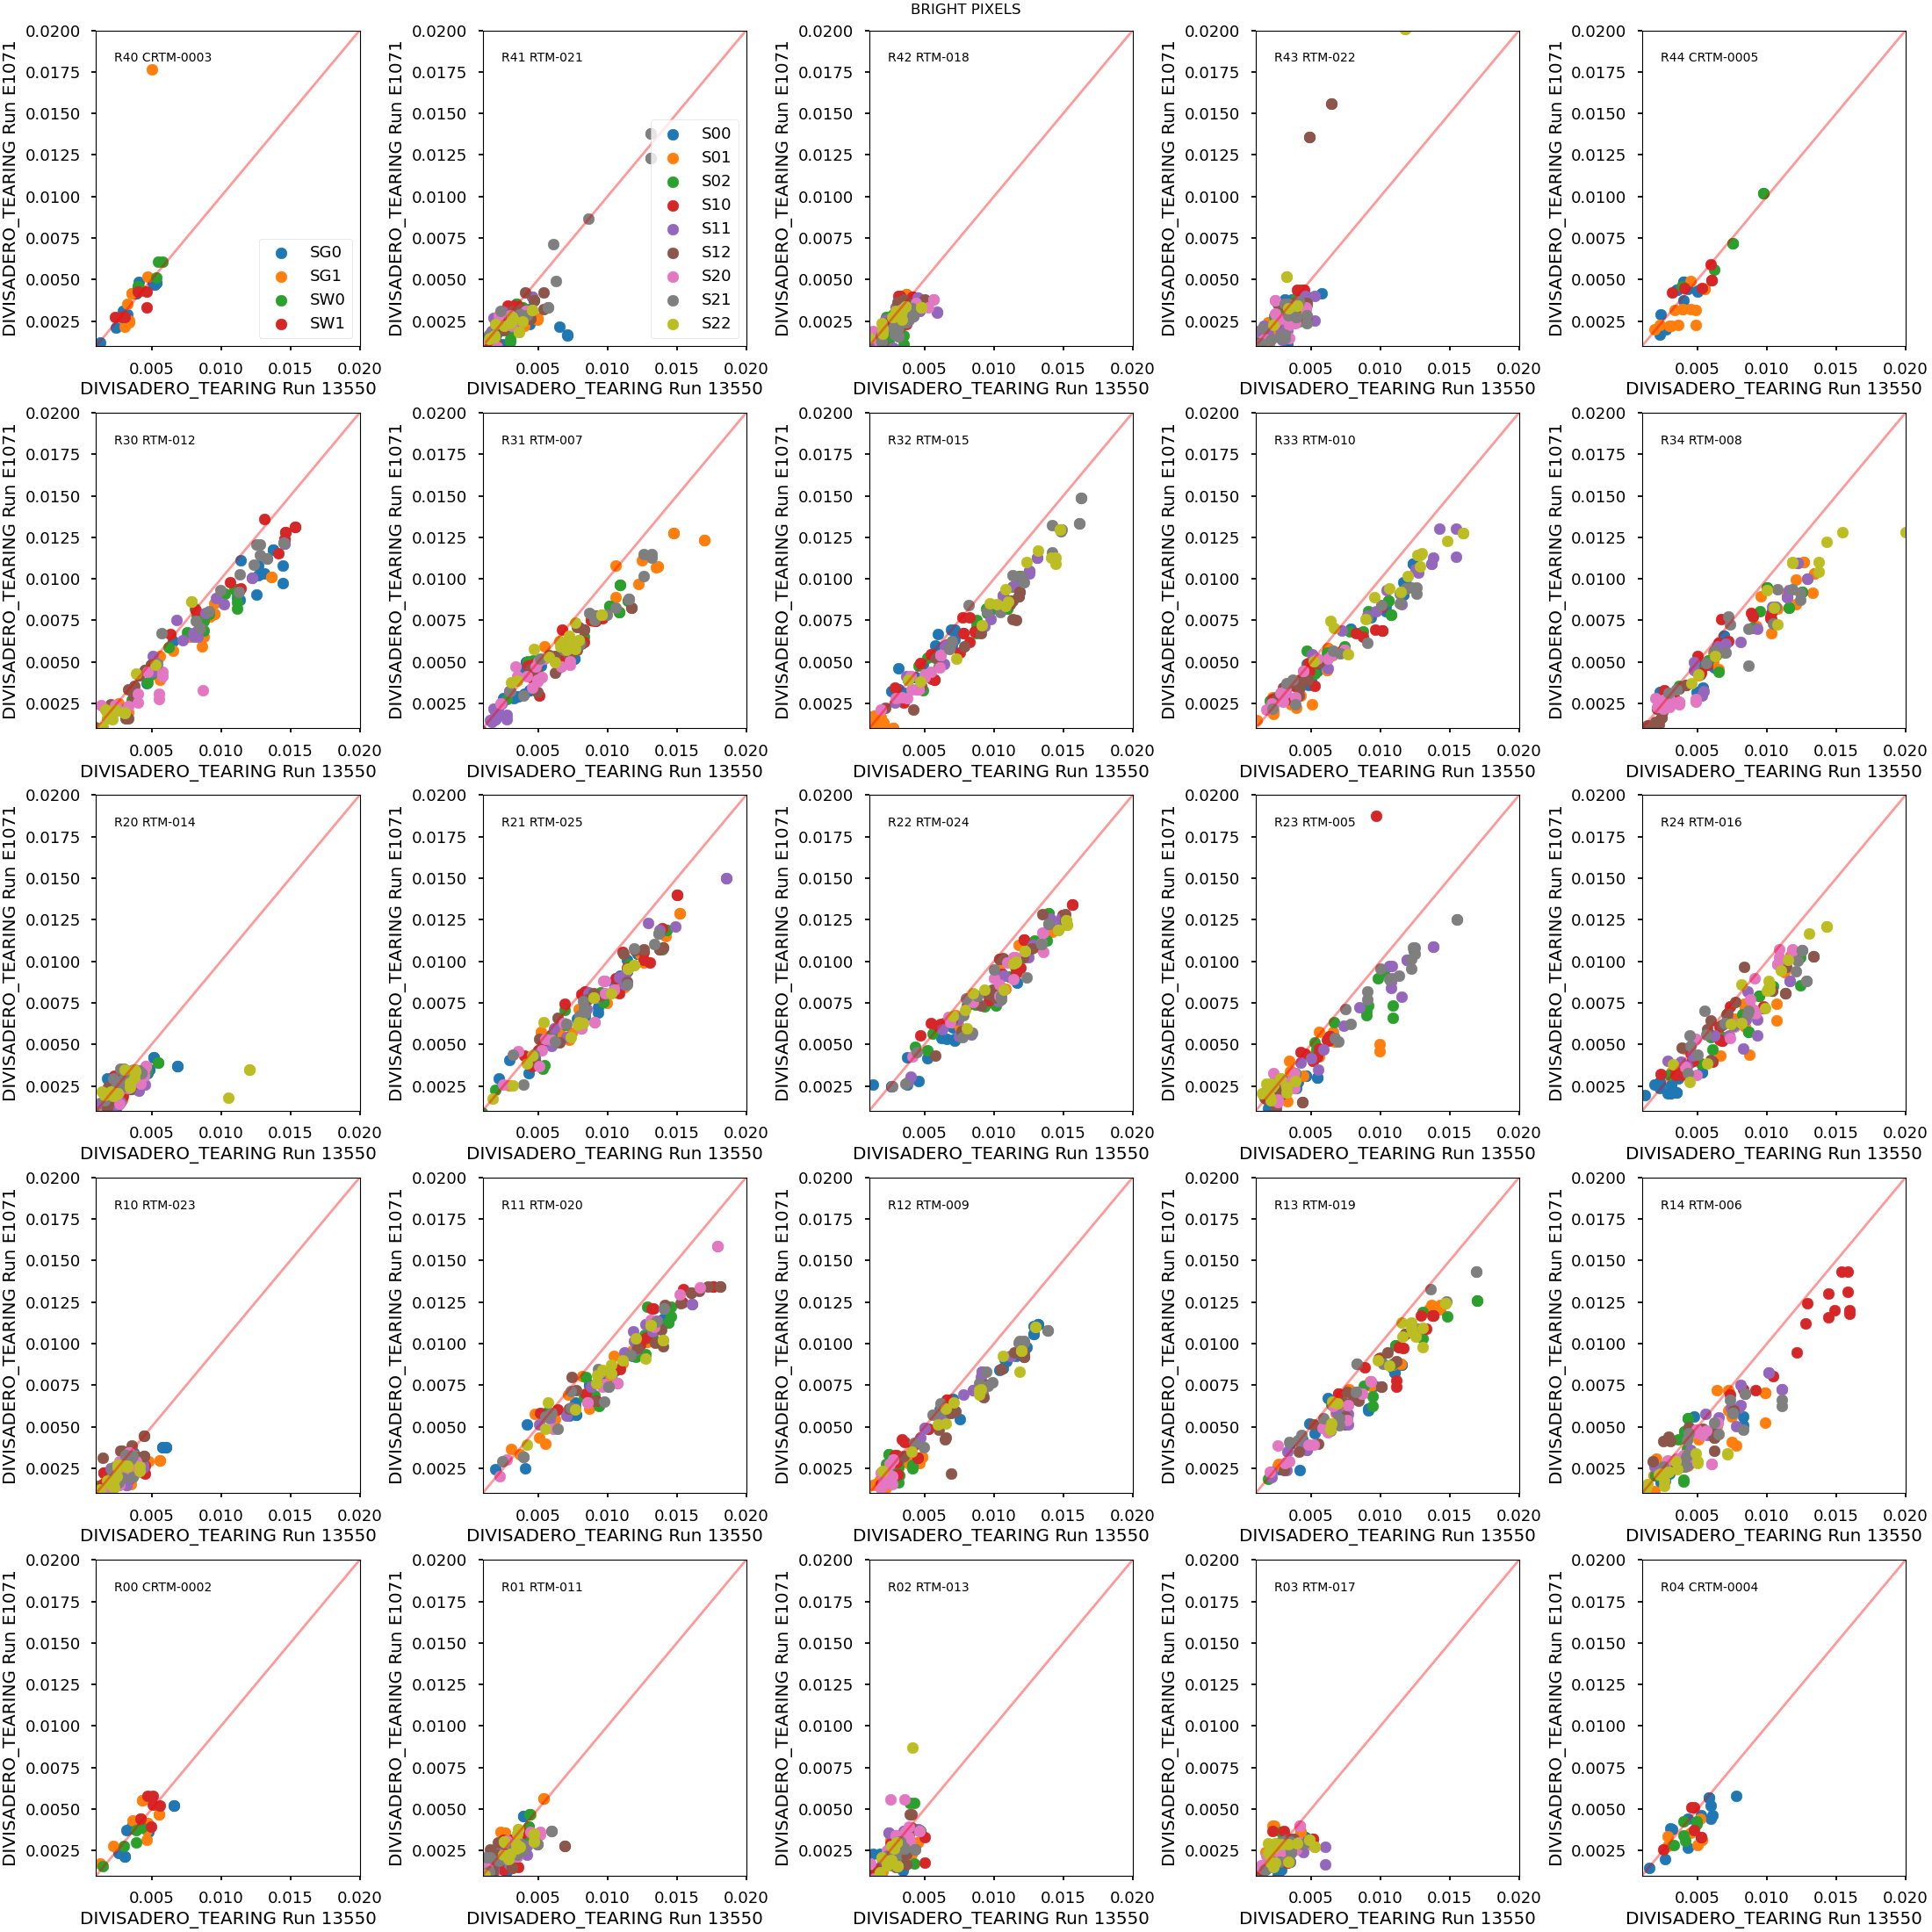
\includegraphics[width=0.5\linewidth]{figures/baselineCharacterization/13550_E1071_DIVISADERO_TEARING_inset.png}
    \caption{Full focal plane measurements of divisadero tearing between runs 13550 and E1071, with populations separated by manufacturer type.}
    \label{fig:ref:eoPipeFP_5x5}
\end{figure}

\clearpage
\subsubsection{Differential histograms}

Another common plot from sections \ref{sec:reverification} and \ref{sec:finalCharacterization} is a histogram, where the counts in histogram bins are differences of amplifier measurements for a given quantity. These histograms are commonly separated by detector type, to show any detector-dependent response. For a consistent measurement, these histograms should be Gaussian centered around zero, with no bias in one direction or another. Distributions that are not centered around zero indicate a change in the measurement between different runs.

\begin{figure}
    \centering
    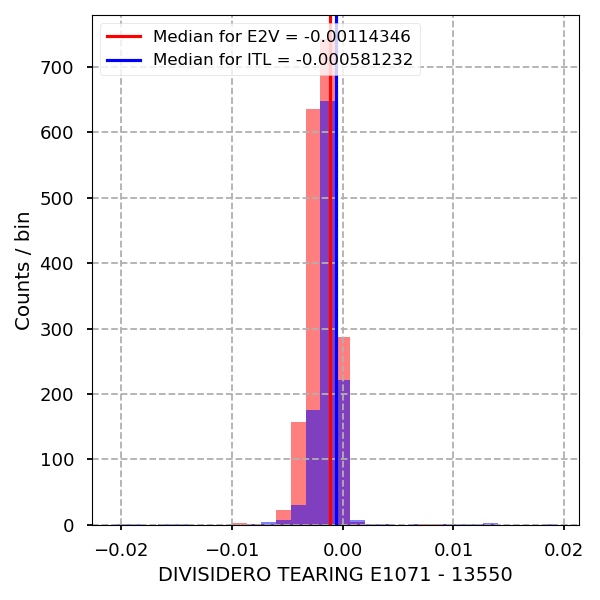
\includegraphics[width=0.8\linewidth]{figures/baselineCharacterization/DIVISIDERO_TEARING_13550_E1071_diff.png}
    \caption{Differential histogram of divisadero tearing between runs 13550 and E1071, with populations separated by manufacturer type.}
    \label{fig:ref:histDiff}
\end{figure}

\clearpage
% \subsubsection{Measurement histograms}
% \subsubsection{PTC curve}

\subsection{Web report reference figures}

A common tool for rapidly reviewing LSSTCam EO data are \href{https://s3df.slac.stanford.edu/data/rubin/lsstcam/}{web reports}, which provide full focal-plane, raft level, and sensor level figures of reference for prompt analysis of data runs. Web reports from runs 6 and 7 are available.

\subsubsection{Focal-plane level}
% \paragraph{Focal-plane layout}

\paragraph{Focal-plane mosaics for different quantities}

Focal plane mosaics consist of fully assembled focal planes, with amplifiers colored according to the associated measurement. The full focal-plane mosaics are generated for most eo-pipe parameters and are scaled appropriately for each parameter. These plots provide a visualization that shows differences in e2v and ITL sensors across the focal plane, and the uniformity.

\begin{figure}[ht]
    \centering
    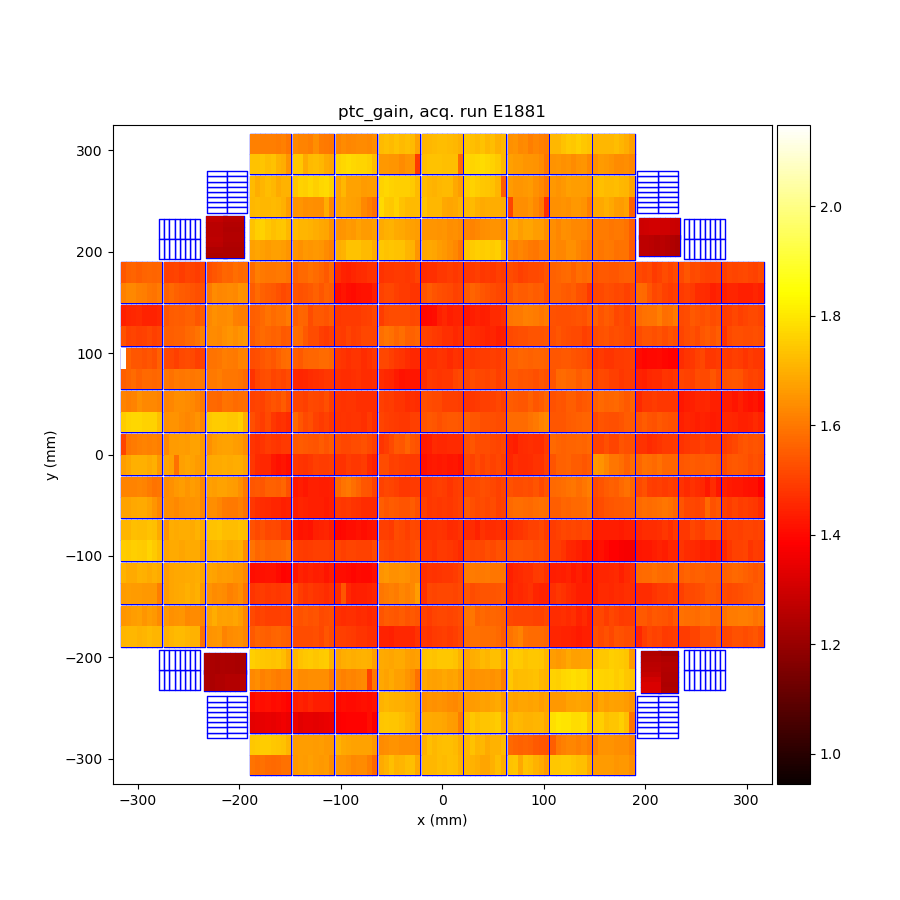
\includegraphics[width=0.7\linewidth]{figures/ReferenceFigures/ptc_gain_plot_LSSTCam_u_lsstccs_eo_ptc_plots_E1881_w_2024_35_20241105T131208Z.png}
    \caption{A focal plane mosaic from run E1881 for PTC gain}
    \label{fig:ref:fpMosaic}
\end{figure}
\clearpage
\paragraph{Histograms}

In addition to focal-plane mosaics, histograms are created for all eo-pipe metrics. These histograms have bins and ranges specific to each parameter. For some parameters, the histograms provide a neat visualization to quantify differences in e2v and ITL measurements, such as figure \ref{fig:ref:histogram} for PTC $a_{00}$. 

\begin{figure}[ht]
    \centering
    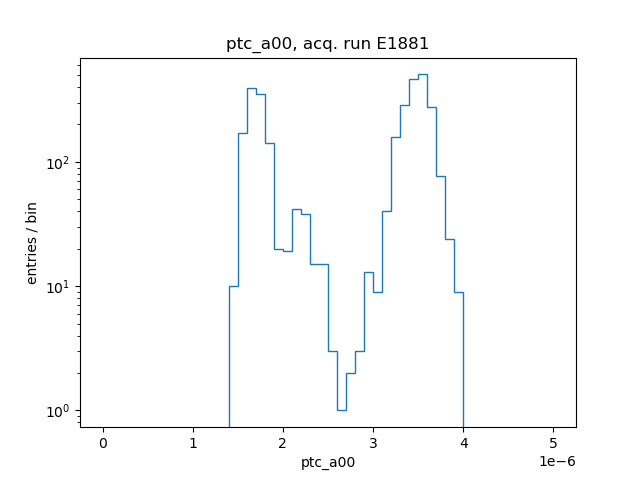
\includegraphics[width=0.8\linewidth]{figures/ReferenceFigures/ptc_a00_hist_LSSTCam_u_lsstccs_eo_ptc_plots_E1881_w_2024_35_20241105T131208Z.png}
    \caption{A histogram from run E1881 for PTC $a_{00}$}
    \label{fig:ref:histogram}
\end{figure}
\clearpage
\subsubsection{Raft level}

\paragraph{Correlation figures}

Correlation figures are created on the raft level for all science rafts. Two types of correlation figures are created; one for the imaging region, and one for the overscan region. The correlation computed is a Pearson correlation coefficient.

\begin{figure}[ht]
    \centering
    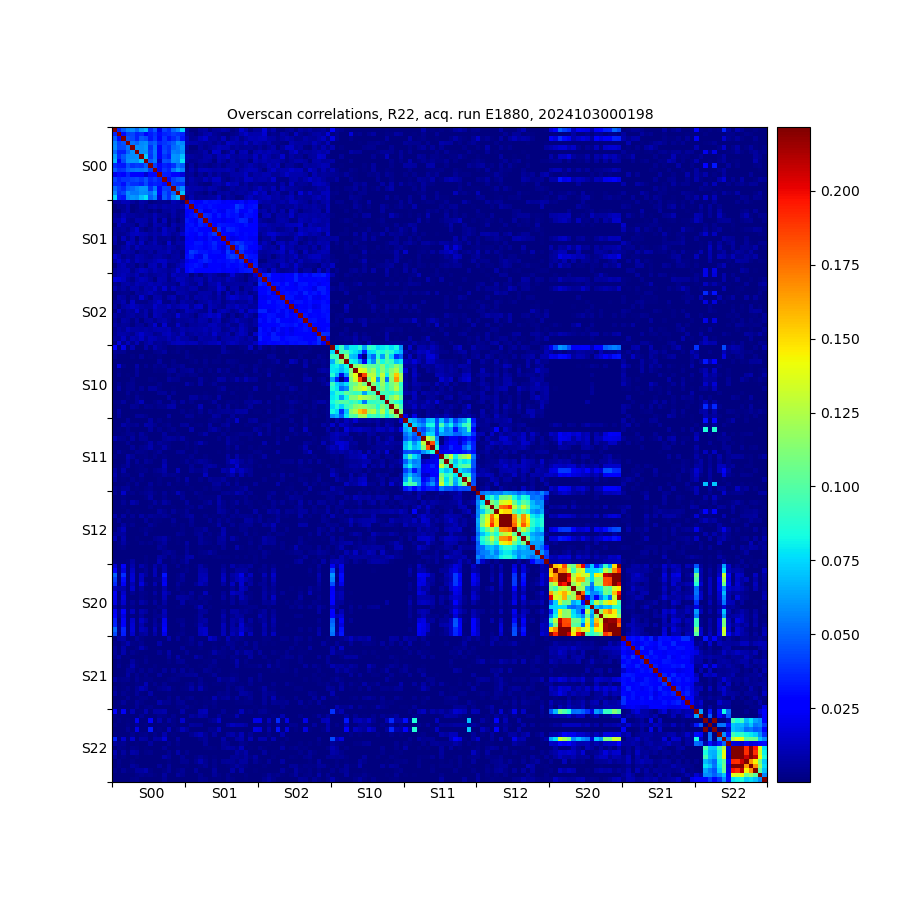
\includegraphics[width=0.8\linewidth]{figures/ReferenceFigures/overscan_correlation_plot_LSSTCam_R22_S00_u_lsstccs_eo_raft_amp_correlations_E1880_w_2024_35_20241101T015955Z.png}
    \caption{Overscan correlations for R22\_S11 in run E1880.}
    \label{fig:ref:overscanCorrelations}
\end{figure}
\clearpage
\paragraph{Lambda mosaics}

As a part of the standard B protocol, flats are taken in different LEDs to provide a chromatic response across the bandpass relevant to LSST. The mosaic is assembled on the raft level, and short wavelength flats show the laser annealing pattern characteristic to e2v sensors (see figure \ref{fig:ref:blueLambda}).

\begin{figure}[ht]
    \centering
    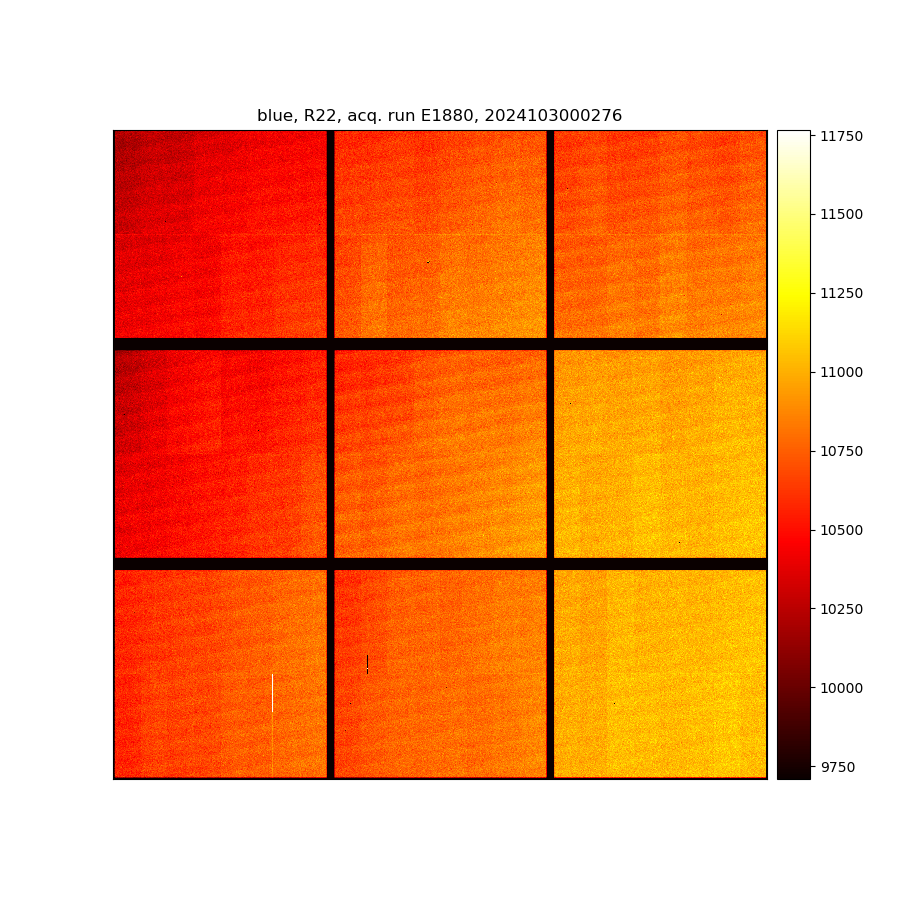
\includegraphics[width=0.8\linewidth]{figures/ReferenceFigures/eoRaftMosaic_LSSTCam_blue_MC_C_20241030_000276_R22_S00_u_lsstccs_eo_raft_lambda_mosaics_E1880_w_2024_35_20241101T020341Z.png}
    \caption{Blue led mosaic for R22 from run E1880.}
    \label{fig:ref:blueLambda}
\end{figure}
\clearpage
\paragraph{Calibration frames}

For runs with bias dark and flat frames (most commonly B protocols), combined calibrations are produced and assembled on the raft level. These mosaics are gain corrected.

\begin{figure}[ht]
    \centering
    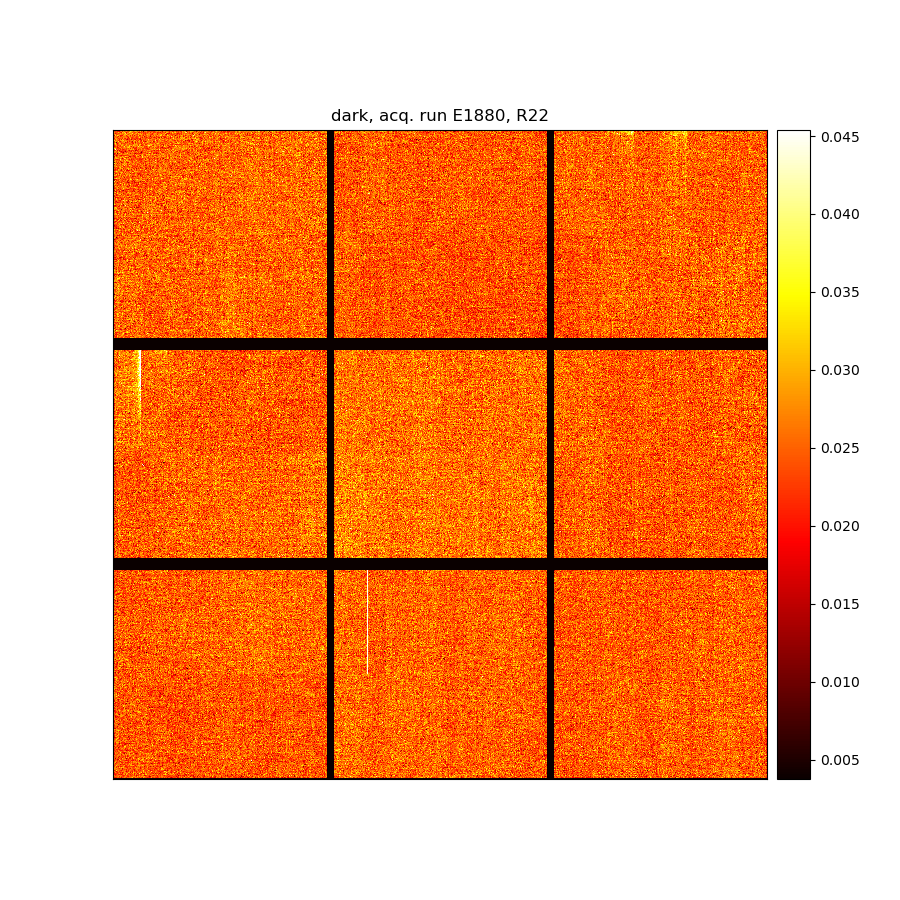
\includegraphics[width=0.8\linewidth]{figures/ReferenceFigures/eoDarkRaftMosaic_LSSTCam_R22_S00_u_lsstccs_eo_raft_calib_mosaics_E1880_w_2024_35_20241101T020324Z.png}
    \caption{Calibration dark for R22 from run E1880, extracted using B protocol dark sequence.}
    \label{fig:ref:calibFrame}
\end{figure}
\clearpage
\paragraph{Bias stability}

Bias stability figures are created for acquisition sequences that acquire multiple bias frames. Three different bias stability plots are created; amp-wise mean vs time, amp-wise standard deviation vs time, amp-wise mean vs time for region covering the readout corner.

\begin{figure}[ht]
    \centering
    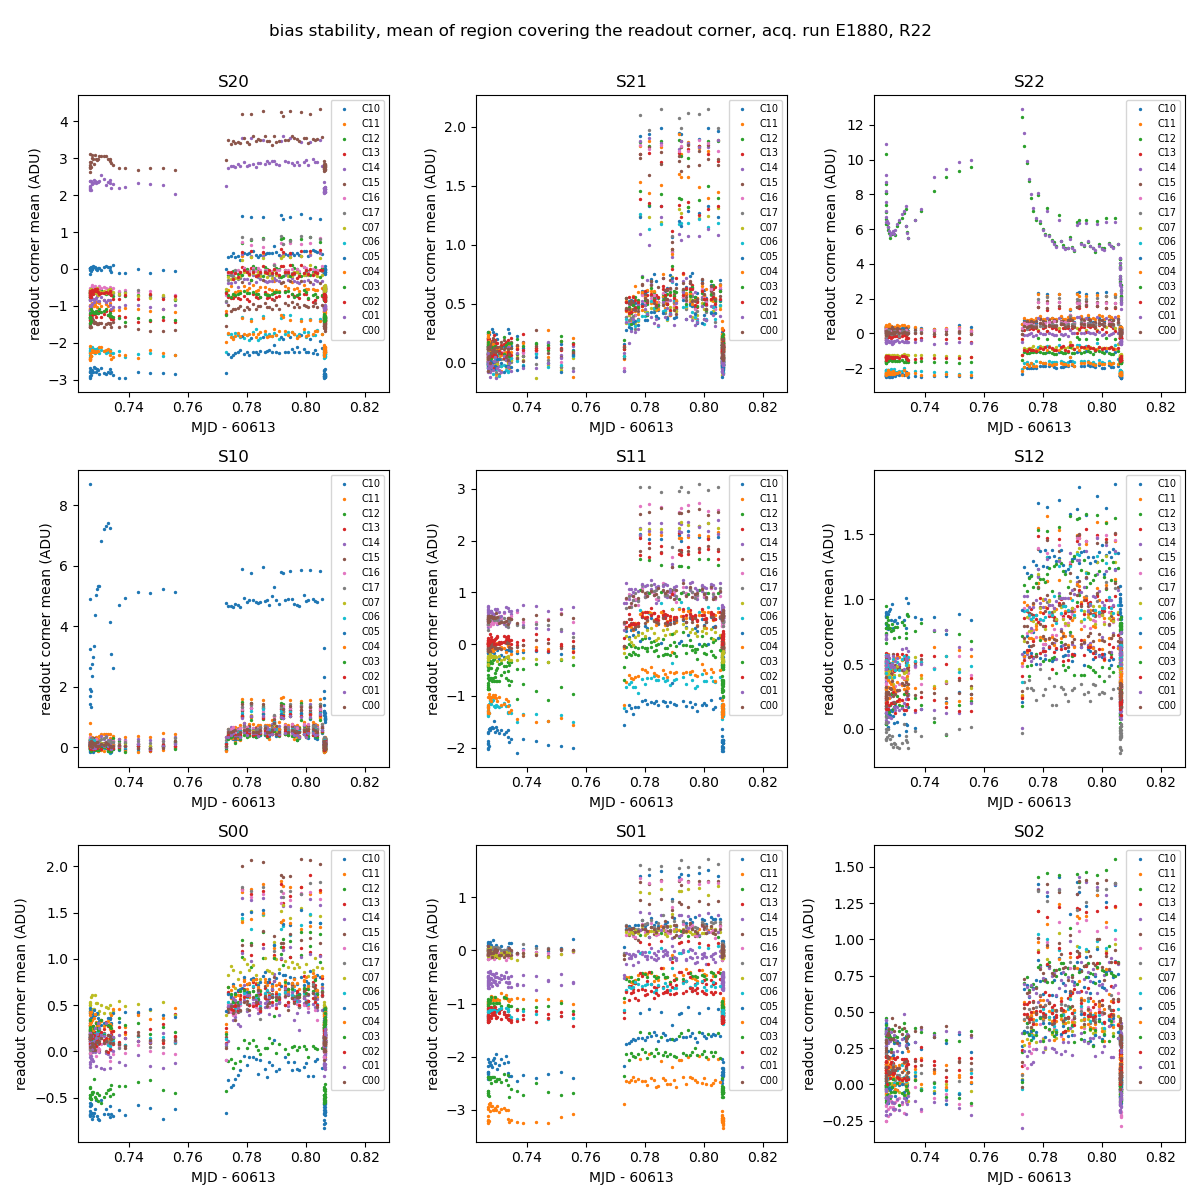
\includegraphics[width=0.8\linewidth]{figures/ReferenceFigures/bias_rc_mean_vs_time_plot_LSSTCam_R22_S00_u_lsstccs_eo_bias_stability_E1880_w_2024_35_20241101T020021Z.png}
    \caption{Bias stability mean vs time in readout corner for R22 from run E1880.}
    \label{fig:ref:biasStability}
\end{figure}
\clearpage
\paragraph{Divisadero profiles}

Divisadero tearing profiles are created for each raft, with divisadero response grouped along the mid-line break. The regions of individual amplifiers are marked by dashed lines to show regions where divisadero response is expected.

\begin{figure}
    \centering
    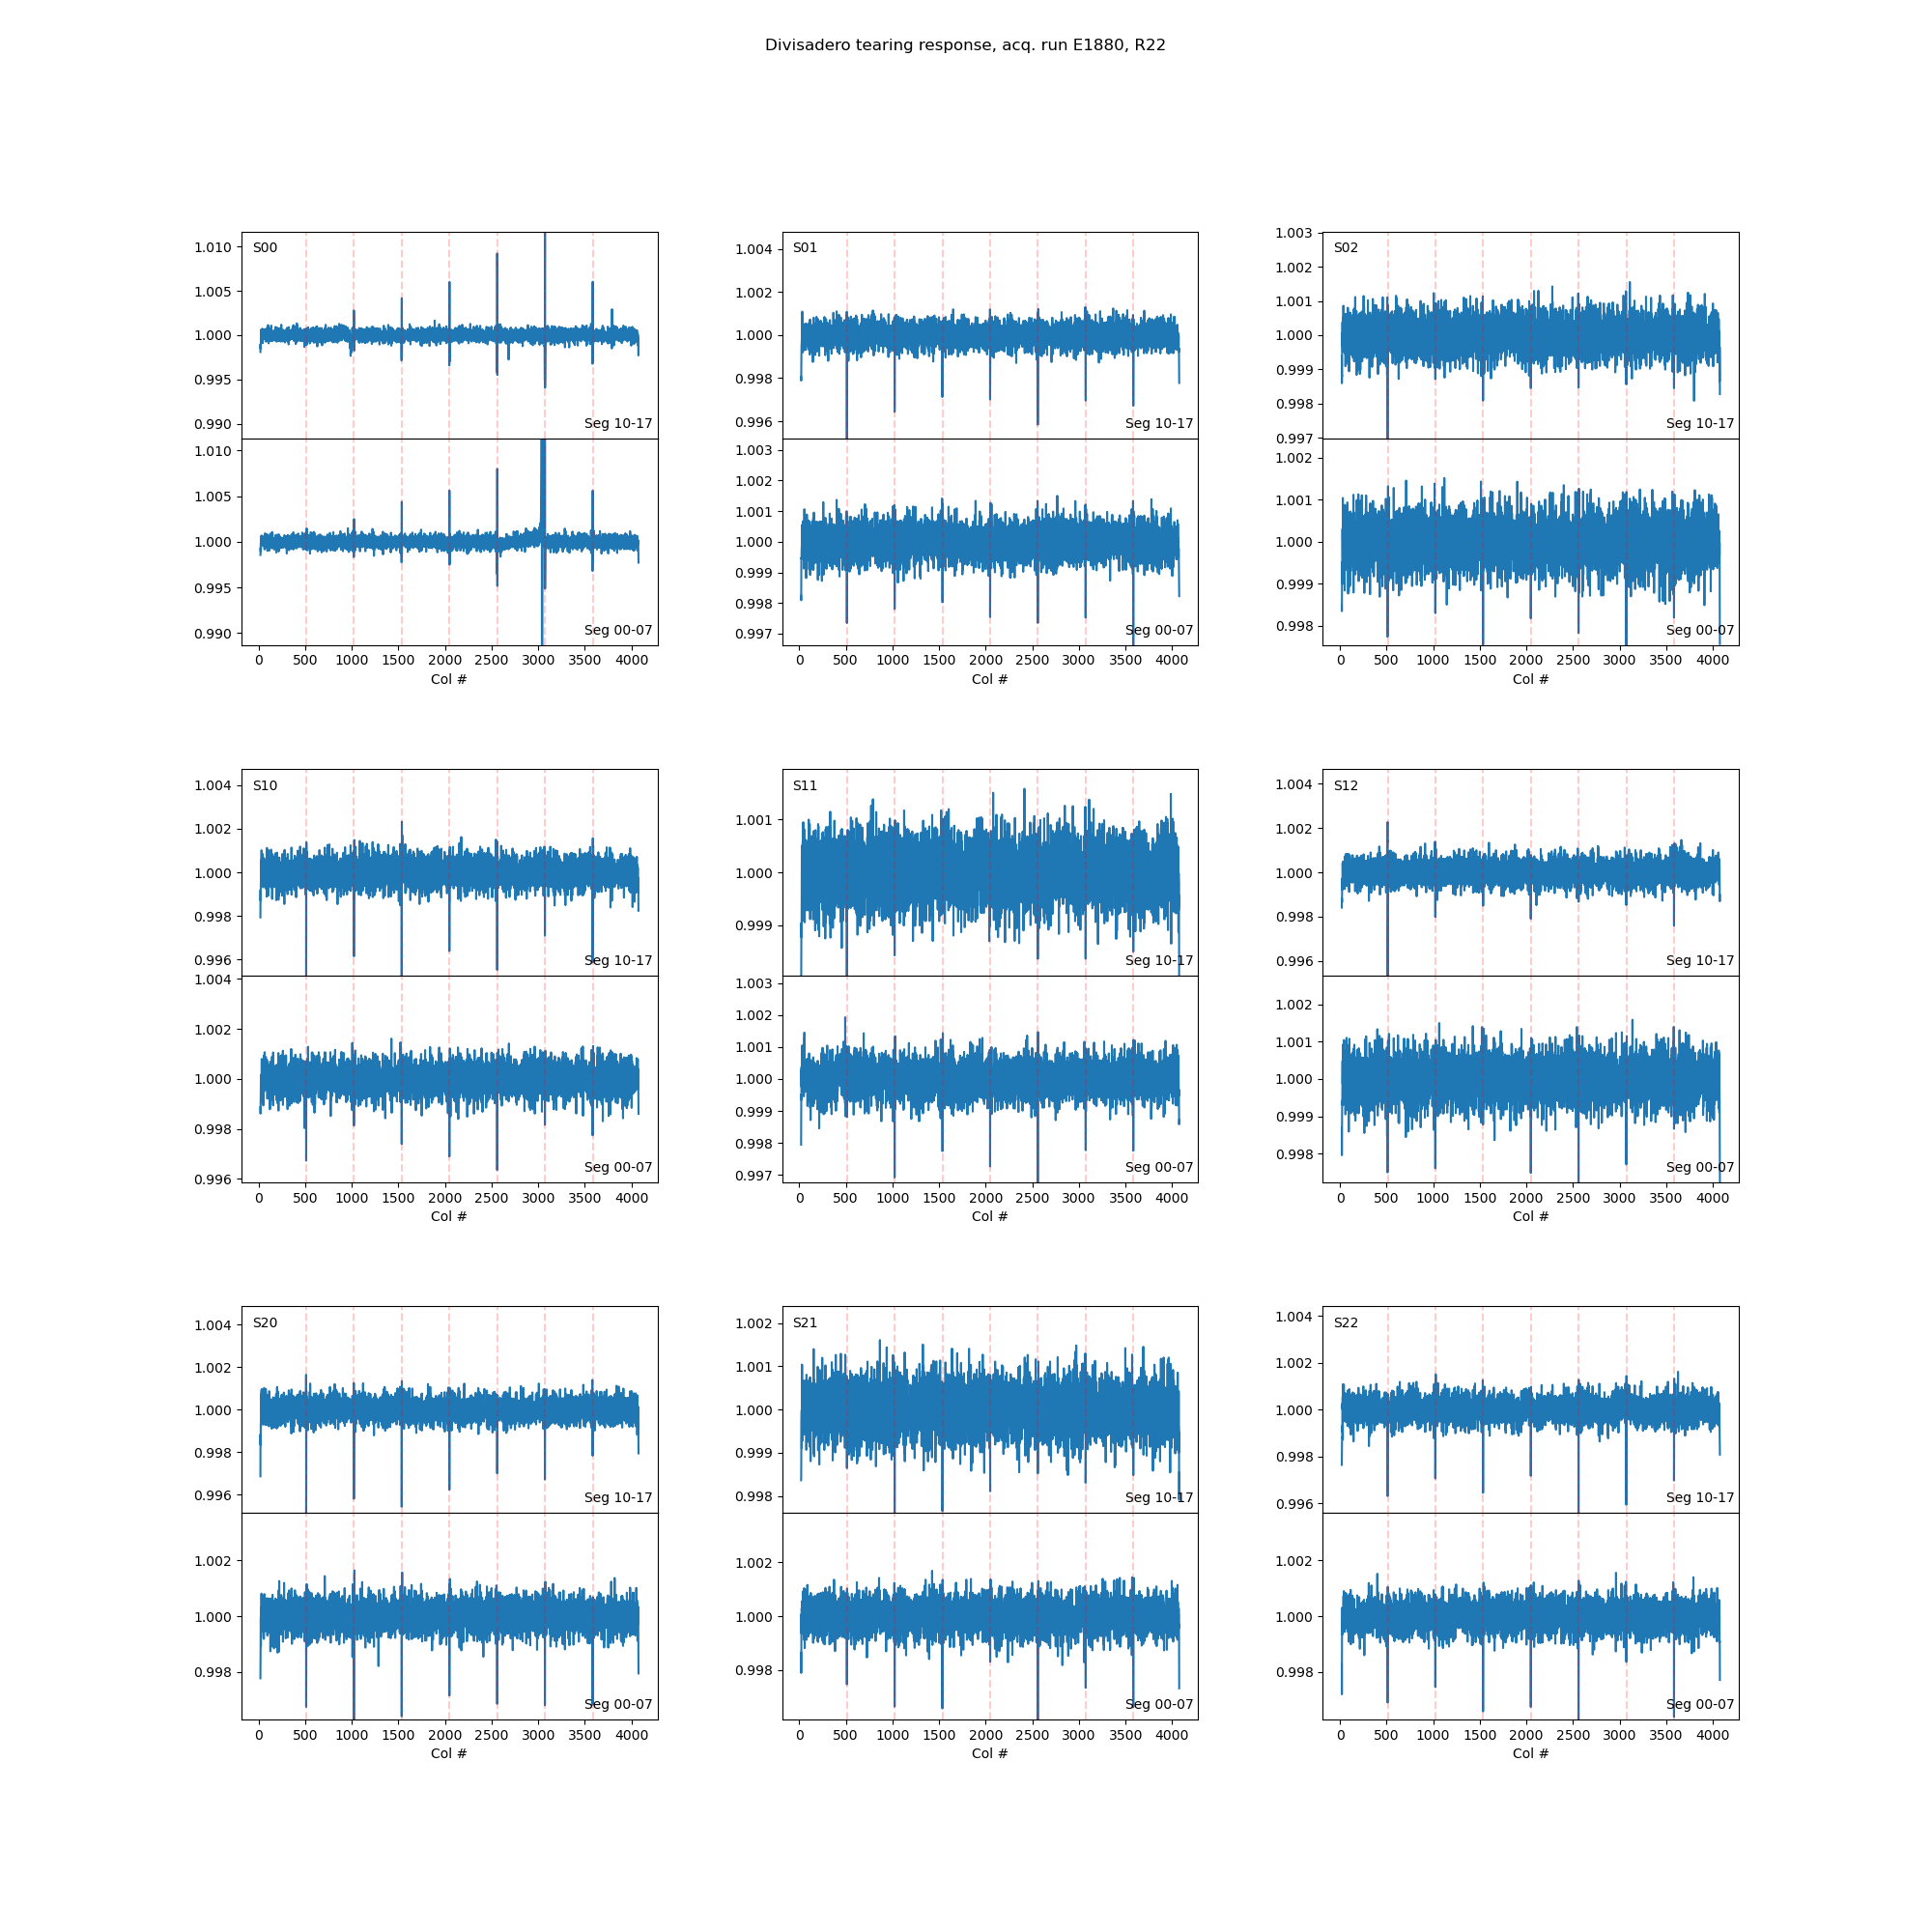
\includegraphics[width=0.8\linewidth]{figures/ReferenceFigures/divisadero_raft_plot_LSSTCam_R22_S00_u_lsstccs_eo_divisadero_tearing_E1880_w_2024_35_20241101T020421Z.png}
    \caption{Divisadero tearing profile for R22 from run E1880.}
    \label{fig:ref:divisaderoProfile}
\end{figure}
\clearpage
\subsubsection{Sensor level}

\paragraph{Bias profiles}

Bias profiles are created for each sensor, along both serial and parallel directions. Amplifiers are plotted separately to allow for amplifier dependent response to be identified. Different columns/rows are plotted in different colors to allow for identification of problematic columns/rows.

\begin{figure}
    \centering
    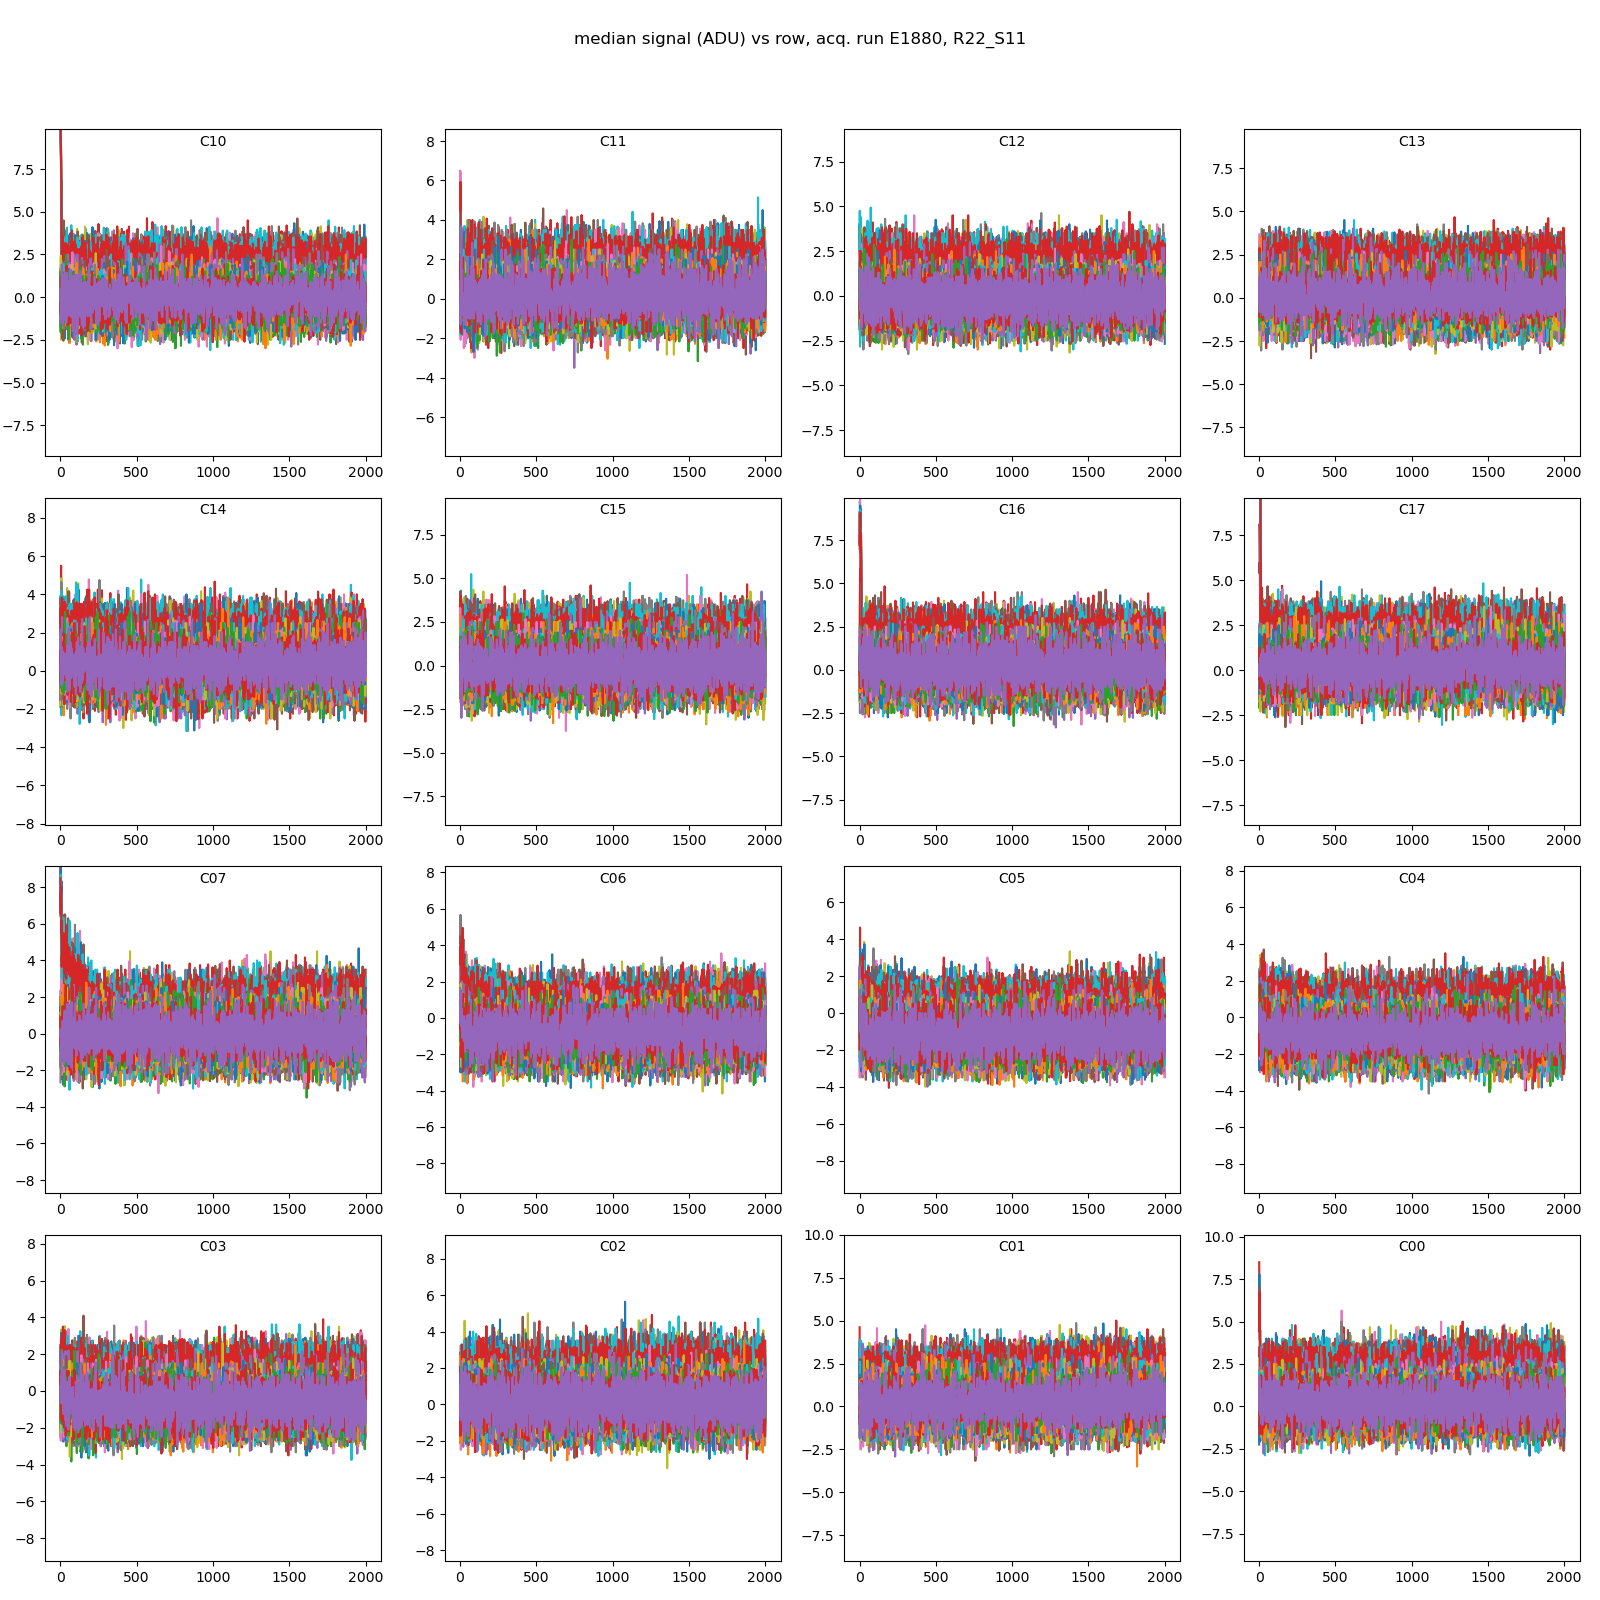
\includegraphics[width=0.8\linewidth]{figures/ReferenceFigures/bias_parallel_profile_plots_LSSTCam_R22_S11_u_lsstccs_eo_bias_stability_E1880_w_2024_35_20241101T020021Z.png}
    \caption{Median bias profile in the parallel direction for R22\_S11 from run E1880.}
    \label{fig:ref:biasProfile}
\end{figure}
\clearpage
\paragraph{PTCs}

PTC plots are created for each sensor, and separated by amplifier. For each amplifier, a PTC curve is created. PTC gain, $a_{00}$, and PTC turnoff (in ADU) is shown for each amplifier. The red points in PTC curves (figure \ref{fig:ref:PTCs}) denote all measurements before PTC turnoff.

\begin{figure}
    \centering
    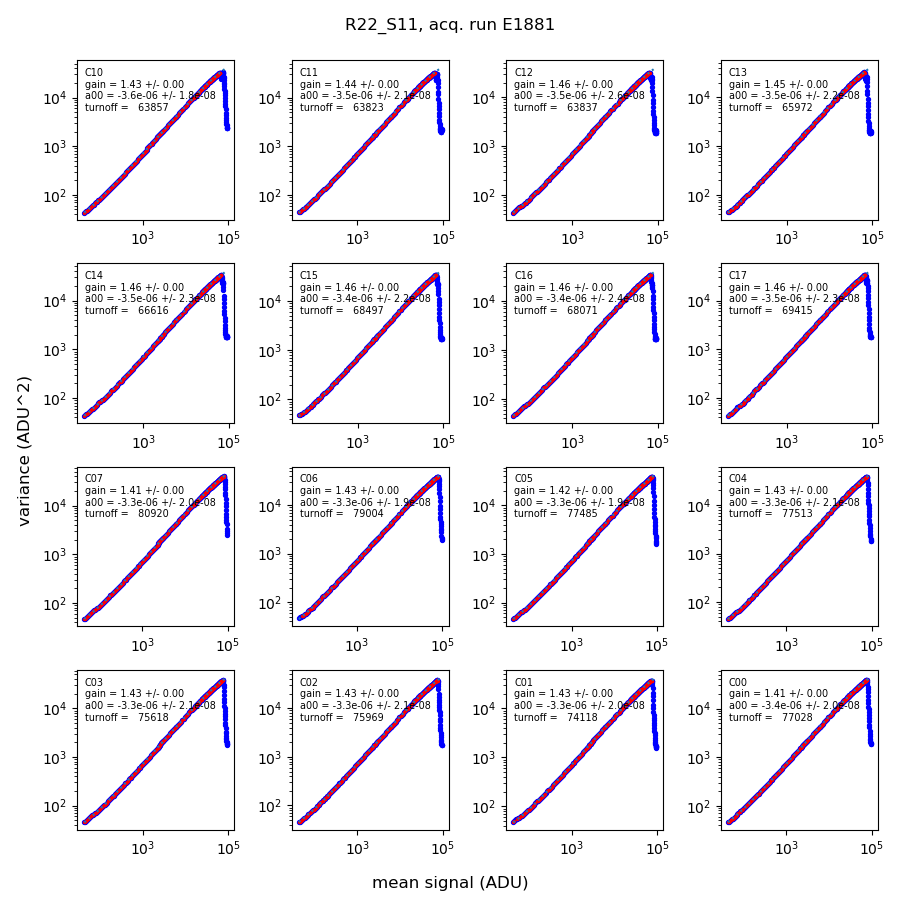
\includegraphics[width=0.8\linewidth]{figures/ReferenceFigures/ptc_plots_LSSTCam_R22_S11_u_lsstccs_eo_ptc_plots_E1881_w_2024_35_20241105T131208Z.png}
    \caption{PTC plots for R22\_S11 from run E1881.}
    \label{fig:ref:PTCs}
\end{figure}
\clearpage
\paragraph{Nonlinearity}

Linearity plots are created for each sensor, and separated by amplifier. For each amplifier, a linearity curve is created showing photodiode current integral vs. e-/pixel for all flat pairs. Maximum fractional deviation, maximum observed signal, and linearity turnoff (in ADU) is shown for each amplifier. The red points in the linearity curves (figure \ref{fig:ref:linearity}) denote all measurements between 100 e-/pixel and linearity turnoff.

\begin{figure}
    \centering
    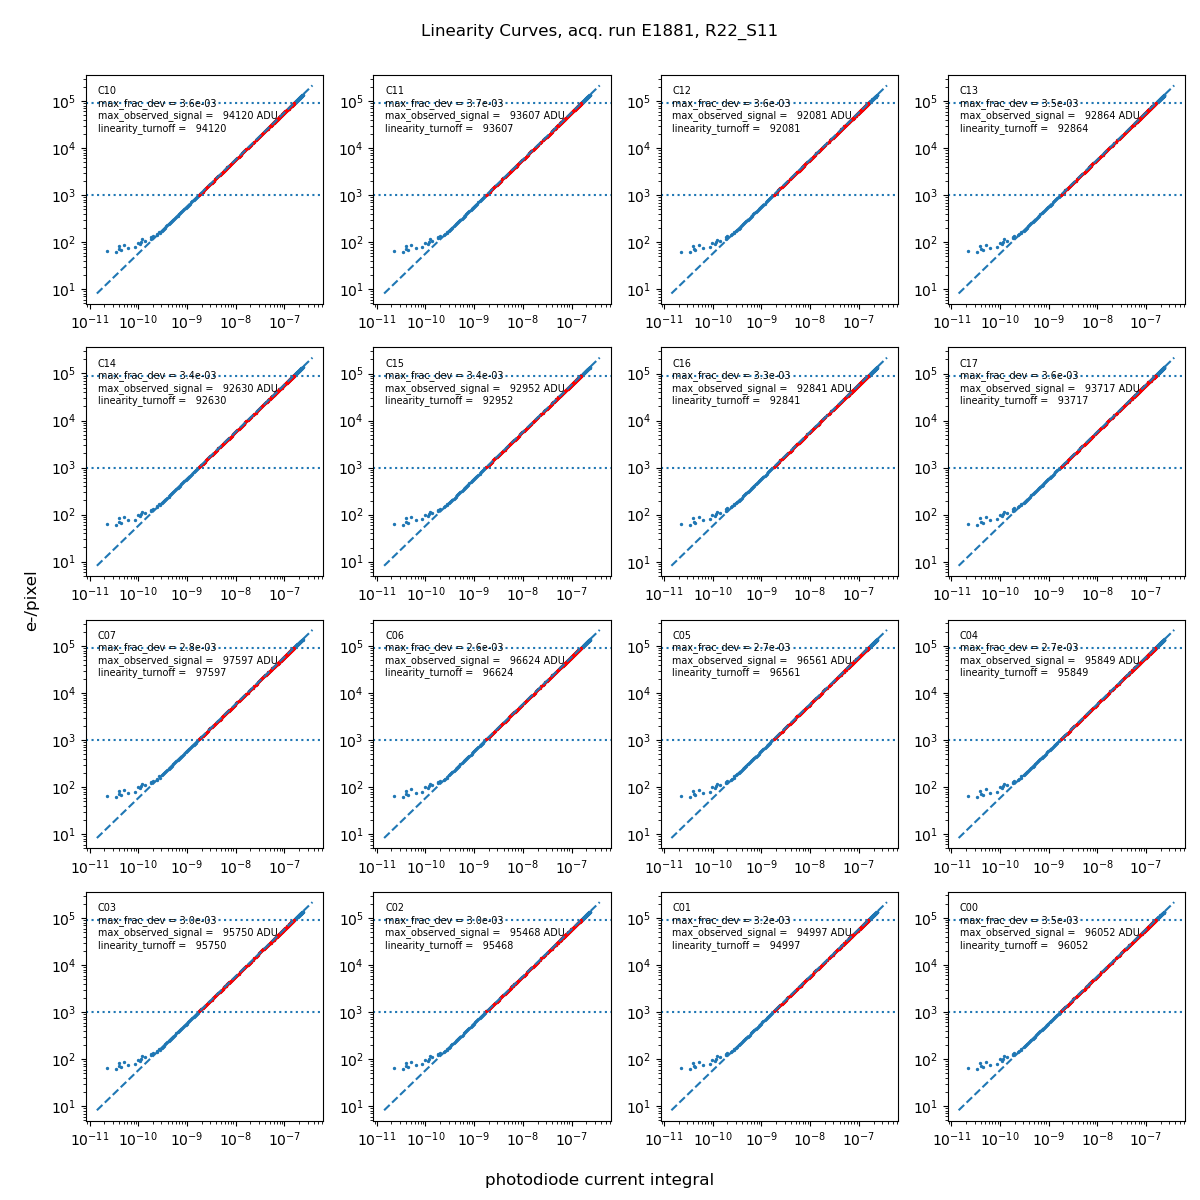
\includegraphics[width=0.8\linewidth]{figures/ReferenceFigures/linearity_fit_plot_LSSTCam_R22_S11_u_lsstccs_eo_linearity_plots_E1881_w_2024_35_20241105T131453Z.png}
    \caption{Linearity plots for R22\_S11 from run E1881.}
    \label{fig:ref:linearity}
\end{figure}
\clearpage
Plots for linearity residuals are also generated, showing the fractional residuals for each amplifier as a function of the photodiode current integral.

\begin{figure}
    \centering
    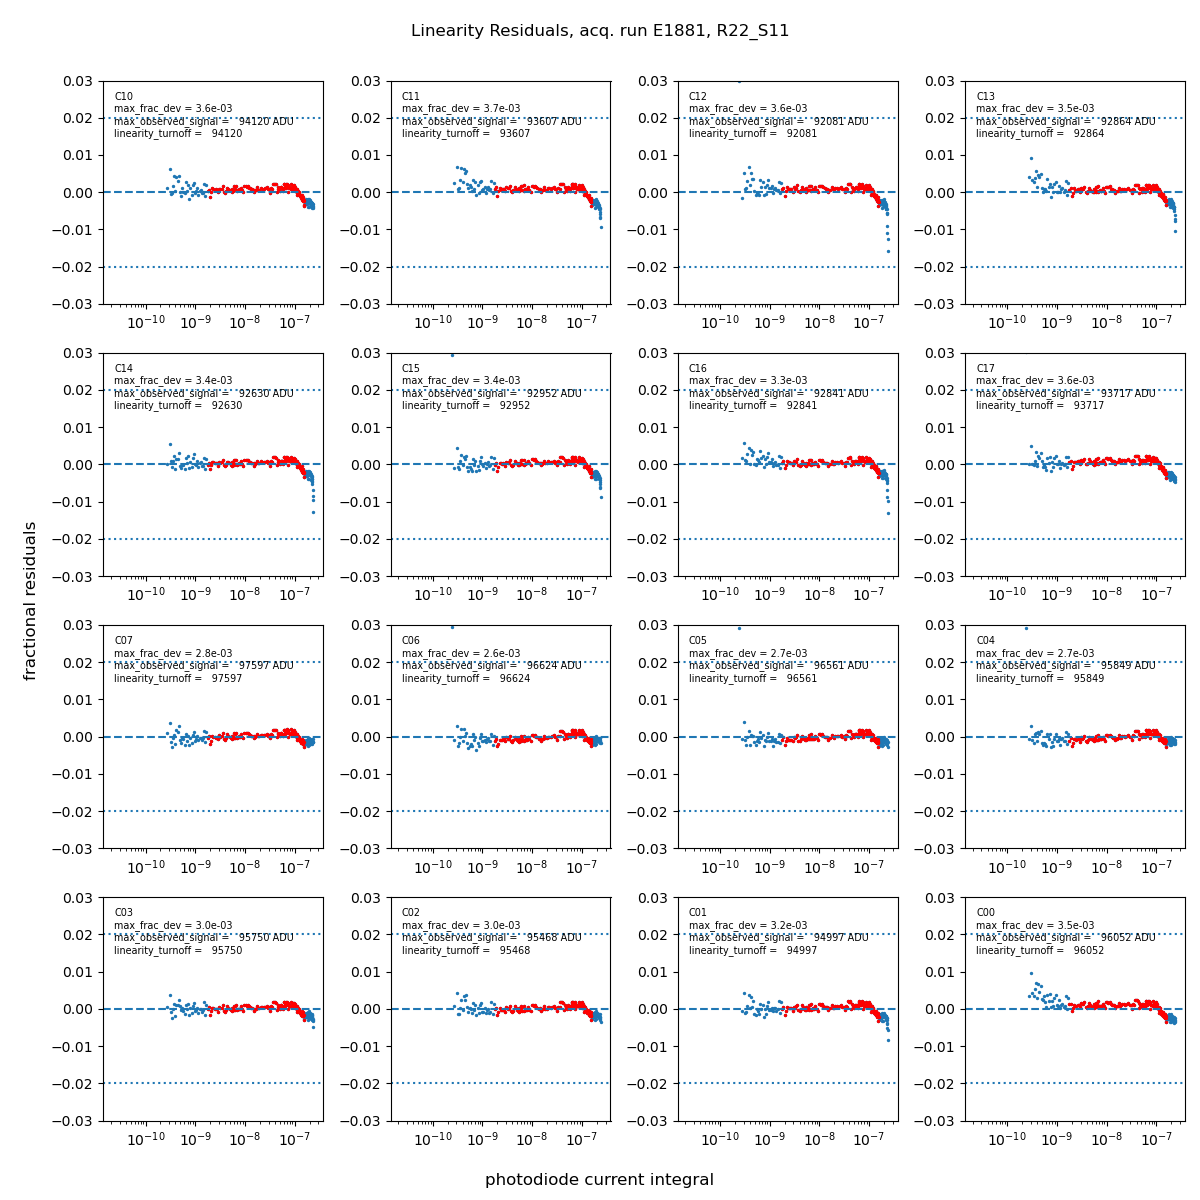
\includegraphics[width=0.8\linewidth]{figures/ReferenceFigures/linearity_residuals_plot_LSSTCam_R22_S11_u_lsstccs_eo_linearity_plots_E1881_w_2024_35_20241105T131453Z.png}
    \caption{Linearity residual plots for R22\_S11 from run E1881.}
    \label{fig:ref:linearityResids}
\end{figure}

\clearpage
\paragraph{Data from flat pairs}

To support studies of row-means variance, a plot showing the row-to-row mean vs. variance of differences between a pair of flats is created. This plot shows different amplifiers in different colors, and allows for identification of changes in correlated noise along with row for individual amplifiers.

\begin{figure}
    \centering
    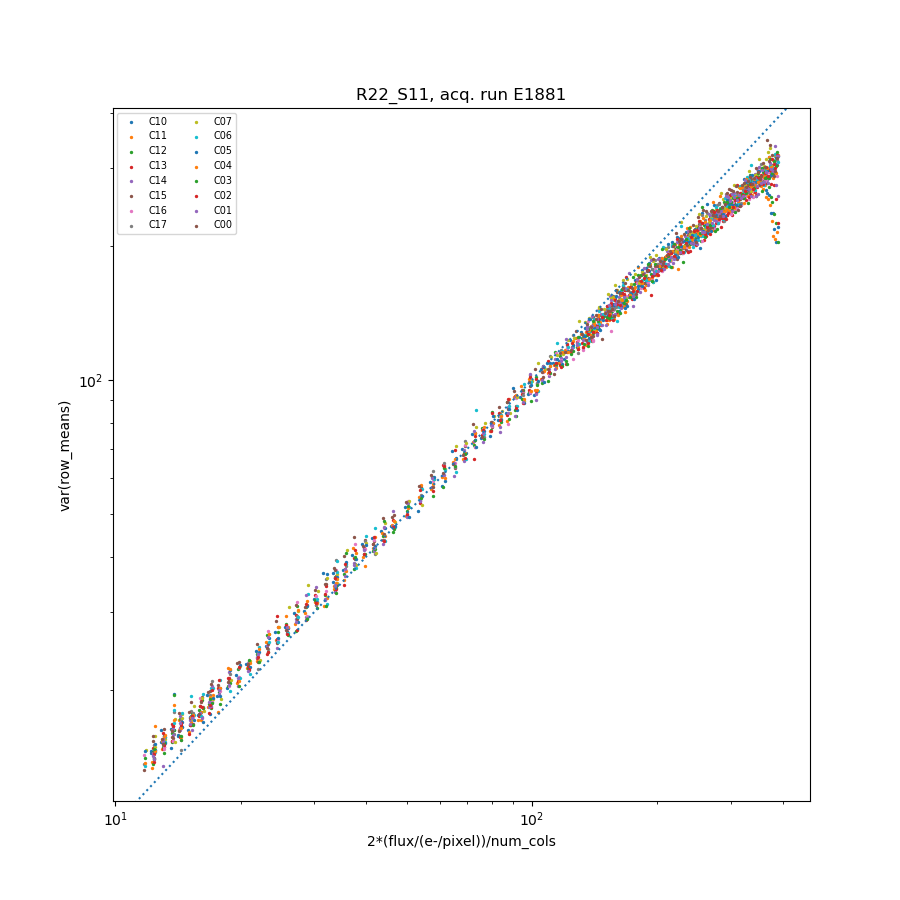
\includegraphics[width=0.8\linewidth]{figures/ReferenceFigures/row_means_variance_plot_LSSTCam_R22_S11_u_lsstccs_eo_ptc_plots_E1881_w_2024_35_20241105T131208Z.png}
    \caption{Row means variance plot for R22\_S11 from run E1880.}
    \label{fig:ref:rowMeansVar}
\end{figure}

\clearpage
\paragraph{CTI}

Plots for showing the charge transfer inefficiency as a function of signal. Different amplifiers are plotted in different colors. CTI plots are generated for serial and parallel CTI.

\begin{figure}
    \centering
    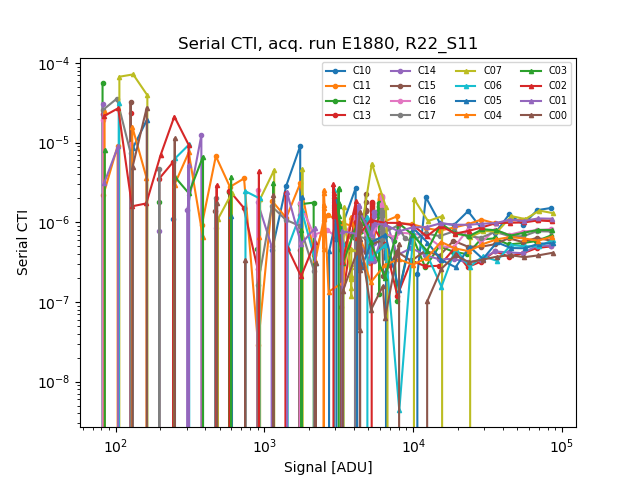
\includegraphics[width=0.8\linewidth]{figures/ReferenceFigures/scti_vs_flux_plot_LSSTCam_R22_S11_u_lsstccs_eo_cti_vs_flux_E1880_w_2024_35_20241101T020455Z.png}
    \caption{Serial CTI plot for R22\_S11 from run E1880.}
    \label{fig:ref:scti}
\end{figure}

\clearpage

\paragraph{BF covariances}

To complement flat pair acquisitions, plots measuring the brighter fatter covariance as a function of flux are generated. Amplifiers are plotted in different colors to easily identify outliers on individual sensors. 

\begin{figure}
    \centering
    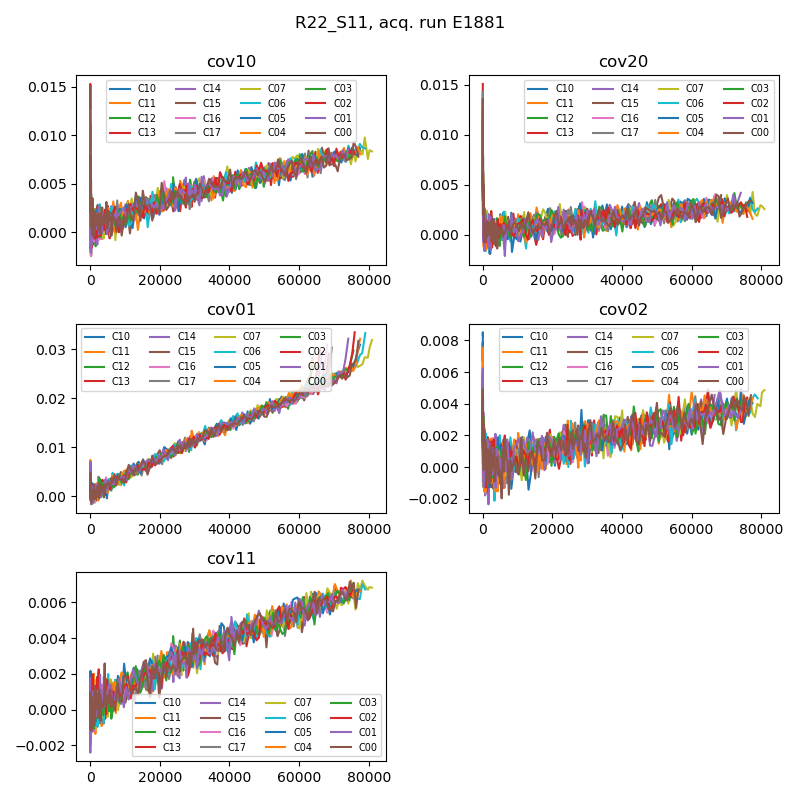
\includegraphics[width=0.8\linewidth]{figures/ReferenceFigures/bf_covariance_plots_LSSTCam_R22_S11_u_lsstccs_eo_bf_analysis_E1881_w_2024_35_20241105T131510Z.png}
    \caption{Brighter-fatter covariance plot for R22\_S11 from run E1880.}
    \label{fig:ref:bfCov}
\end{figure}

\clearpage
\paragraph{Persistence}

B protocols include a persistence acquisition, which is a saturated flat (usually at 400k e-), followed by a sequence of multiple 15 sec dark images. To complement this image acquisition, persistence plots are generated that show the decay of residual signal in the dark sequence. These plots are in units of ADU, and are color coded according to each amplifier.

\begin{figure}
    \centering
    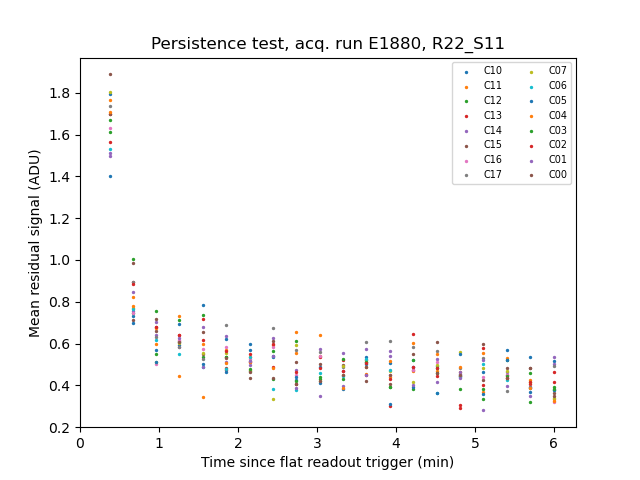
\includegraphics[width=0.8\linewidth]{figures/ReferenceFigures/persistence_plot_LSSTCam_R22_S11_u_lsstccs_eo_persistence_E1880_w_2024_35_20241101T020526Z.png}
    \caption{Persistence plot for R22\_S11 from run E1880.}
    \label{fig:ref:persistence}
\end{figure}

\clearpage
\section{OCS integration}
A secondary goal of the run 7 campaign is further testing of integration between the Camera Control System (CCS) and the Observatory Control System (OCS). The tests performed with OCS control of LSSTCam during this campaign are the first operations of the LSSTCam with OCS which will be the normal operating mode during operations of the Simonyi Survey Telescope. To this end, many tests were performed during the Run 7 campaign including basic functionality tests, short OpSim runs, long, scheduler-driven OpSim runs ("survey mode") and the start of mock calibrations.

%\subsection{LSSTCam in OCS}

\subsection{Testing steps and achievements in Run 7}
OCS testing with LSSTCam was part of three steps of the Run 7 campaign. Prior to starting any of the steps, basic functionality was confirmed with single exposures via an OCS script. The first image taken with OCS happened on September 13th, 2024 early in the campaign to give time to address potential issues. The 3 steps with OCS driven operation where then as follows:
\begin{itemize}
    \item 30 minute OpSim runs. These were pre-generated sequences pulled from survey simulations including filter changes and different observation strategies for different filters, which may be a feature of the LSST survey. Two runs were successfully completed: E1414 which included operation of the shutter and E1585 which did not operate the shutter.
    \item Fully scheduler driven OpSim runs. These runs used the Rubin Scheduler to dynamically choose targets, filter changes and exposure times depending on the filter. The scheduler was configured to choose targets at any time - not only with the sun down - and to only operate LSSTCam and not point the telescope, though simulated slew times were added. 
    \item A run of an example calibration sequence that could be run as part of a daily calibration sequence. This was intended to include testing image ingestion and processing of the calibrations with the observatory control system.
\end{itemize}

Together, these steps demonstrated the ability to operate LSSTCam in a mode similar to what night time operations are anticipated to be like in a steady state. The listed acquisitions include over 12 hours of operation under control of the OCS including filter changes, shutter operation, guider ROI setting and variable exposure times. These operations also included simulated slew times. Image acquisition also worked in conjunction with the observatory header service to populate image headers with additional details and telemetry from the observatory.

While testing was largely successful, some issues were encountered and resolved along the way. One issue was that the interface for sending guider regions of interest (ROIs) through the OCS was incomplete. The initial interface was developed and tested as part of this process. The sending of guider ROIs revealed another issue with command acknowledgments between the camera OCS bridge and the scripts operating the system.  


\subsection{Further testing and development}
Not all testing goals to verify the Camera-OCS interface were possible during Run 7. A future testing period for lingering items is planned in February or March, 2025 to close the loop on the remaining tests. These tests will use playlists and playback of data taken during Run 7.

An item to test is the summit storage facility for operations (S3), which was not yet available. With the playback mode testing, we will verify proper ingestion of images into S3.

Another open item to be tested is a complete loop of calibrations being processed with the Observatory Control Pipeline Service (OCPS) immediately after their acquisition. A calibration playlist is included as part of the planned OCS testing period. With this data can be collected and sent to the OCPS to verify near real time processing of calibrations.

Lastly, between Run 7 and the first photon of LSSTCam, the observatory changed the communication middleware software used within the OCS. The change from DDS to Kafka is expected to improve stability of the communication between distributed software components of the OCS. For LSSTCam, the playback testing will be used to test if both general performance in the new middleware environment, and to see if missing command acknowledgments found in Run 7 remain reproducible. 

\clearpage
\section{Phosphorescence}\label{appendix:phosphorescence}
Because we have discovered the phosphorescence in ITL sensors only recently, we have here cobbled together the data products described here. We believe they are appropriate for quantitative characterization of these systematics that are essentially a position dependent hysteresis indexed by recent illumination history. 

Happily, the {\it front side persistence} seen in e2v sensors has been strongly suppressed with only parallel clock swing voltage adjustment ({\it cf.} Fig.~\ref{fig:ref:persistence} for post-mitigation performance). Although the working assumption of the {\it e2v persistence} was that it affected all pixels identically, this has not been demonstrated, and only sensor-averaged {\it persistence} expression were evaluated to date. The current, post-mitigation {\it persistence} performance ({\it cf.} Fig~\ref{fig:finalChar-persistenceAllLEDs}) provide indirect evidence of the spatial dependence to the {\it persistence}, revealed in the {\it skew} of the distributions quantified:\footnote{NB. It is still difficult to disentangle true {\it persistence} from residual charge read out following {\it clear} operations with finite inefficiency. However, it is believed that operating with {\bf NopSf} removes nearly all residual signal resulting from incomplete clear.} Especially with {\it y-band} illumination, the significant skew apparently indicates pixel-to-pixel variation in persistence, which has not yet received adequate attention as a mechanism that would fall within ISR scope.

The {\it phosphorescence} seen in ITL sensors is highly position dependent as compared to the {\it front side persistence}. This was first revealed plainly in the morphology of post-illumination dark images of R43\_S11 ({\it cf.} Fig.~\ref{subfig:hvb_on_R43_S11}) and R00\_SW1 ({\it cf.} Fig.~\ref{fig:phos:stains}). Clearly, the methodology of {\it persistence} estimation feedback, used while tuning clock swing, is not suitable for quantifying {\it phosphorescence} in parts of the focal plane covered by ITL sensors.

The data products displayed in the following sections are described here:
\begin{itemize}
    \item[$\ast$] Identification phosphorescent regions (Appendix \ref{appendix:phos:ident}): Using the 20 B-protocol runs containing the {\it BOT PERSISTENCE} set of images, we constructed pixel-by-pixel median images over the 20 instances of the {\it first} post-flash {\bf dark} image, and also for the {\it twentieth} post-flash {\bf dark} image. The difference between the two ({\it first} minus {\it twentieth}) is 8x8 blocked and displayed on a raft-by-raft basis. Such pixels appear significant when they contain (on average) 10e$^-$ of transient signal within the first 15s dark.
    \item[$\ast$] Comparison against {\it blue} flat field response (Appendix \ref{appendix:phos:coffeestains}): The same {\it transient term} images described above are displayed {\it without} blocking, no rebinning. These were inspected alongside the {\it blue} flat field response images to estimate whether {\it coffee stain} and {\it vampire pixel} features are consistently correlated with phosphorescent regions. (No for {\it coffee stains}, yes for {\it vampire pixels}.)
    \item[$\ast$] Kinetics characterization (Appendix \ref{appendix:phos:kinetics}): Pixel-by-pixel median images constructed with the 20 {\it BOT PERSISTENCE} datasets were constructed for each of the 20 successive dark images following the flash (trigger) exposure. These data products did not subtract the twentieth median image from each, but were kept intact. Using ROI pixel extractions and signal level quantile estimations, we extract high significance evolution of the transient signal, with the understanding that different pixels may be driving each time slice's quantile level. In principle, this could be repeated for each pixel in the focal plane to generate a short list of parameters modeled after the function given in Fig.~\ref{fig:phos:kinetics:fit:R20S20C13}\footnote{These results are expected to be sensitive to details of the {\it trigger} exposure and where it is placed temporally within the exposure duration. We currently do not have such transient functions measured after illumination exposure defined by the Camera Shutter's {\it open} duration.}. Evolution of the actual cumulative distributions for a selection of ROIs are provided.
    \item[$\ast$] Response characterization (Appendix \ref{appendix:phos:response}): The acquired data available to address phosphorescence response to illumination (wavelength and signal level in the trigger as independent variables) were marginally adequate to estimate the {\it amplitude only} of a putative decay profile resembling Fig.~\ref{fig:phos:kinetics:fit:R20S20C13}. We did not have 20 {\it BOT PERSISTENCE} datasets from which to construct median images, and so worked only with the single instances available (specifically, only the first dark image following flash). Variations from ROI to ROI in the phosphorescence response are clearly seen across the independent variable plane (illumination wavelength and signal level)\footnote{Note that ROI extractions from single dark images such as these are susceptible to cosmic rays. The 99\% quantile level applied to the extraction also gets pegged to the noise distribution at about $3\sigma$ when the product of phosphorescent response and trigger illumination level is small.}.
\end{itemize}


\clearpage
\section{Phosphorescence identification on ITL set of sensors}

\begin{figure}[!htbp]
\centering
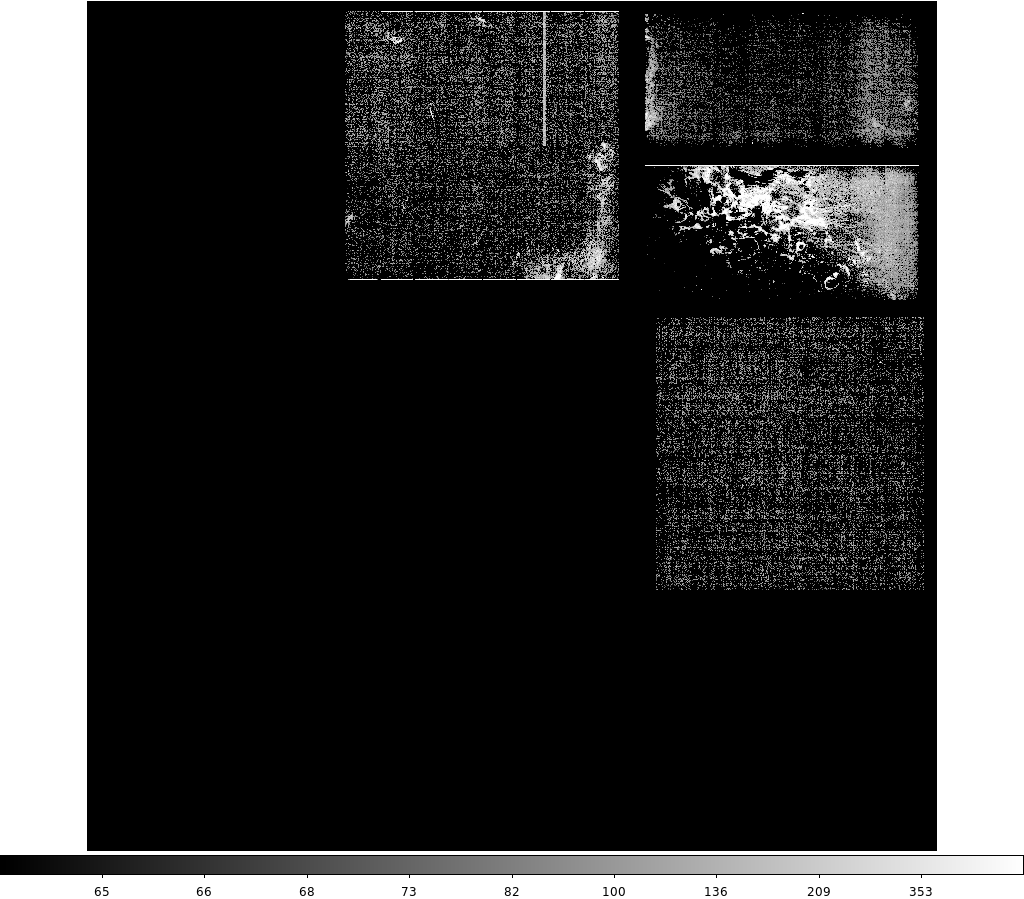
\includegraphics[width=0.9\textwidth]{figures/phosphorescence-survey/itl_fluor_R00_0-19_rb1_log.png}
\caption{Phosphorescence transients for the R00 CRTM captured in the first 15\,s following {\it red} CCOB LED at 400\,ke$^-$/pix. With 8$\times$8 blocking, the upper end of the color scale (640) corresponds to 10\,e$^-$/pixel when averaged over 64 pixels contributing.}
\label{fig:phos:R00}
\end{figure}

\begin{figure}[!htbp]
\centering
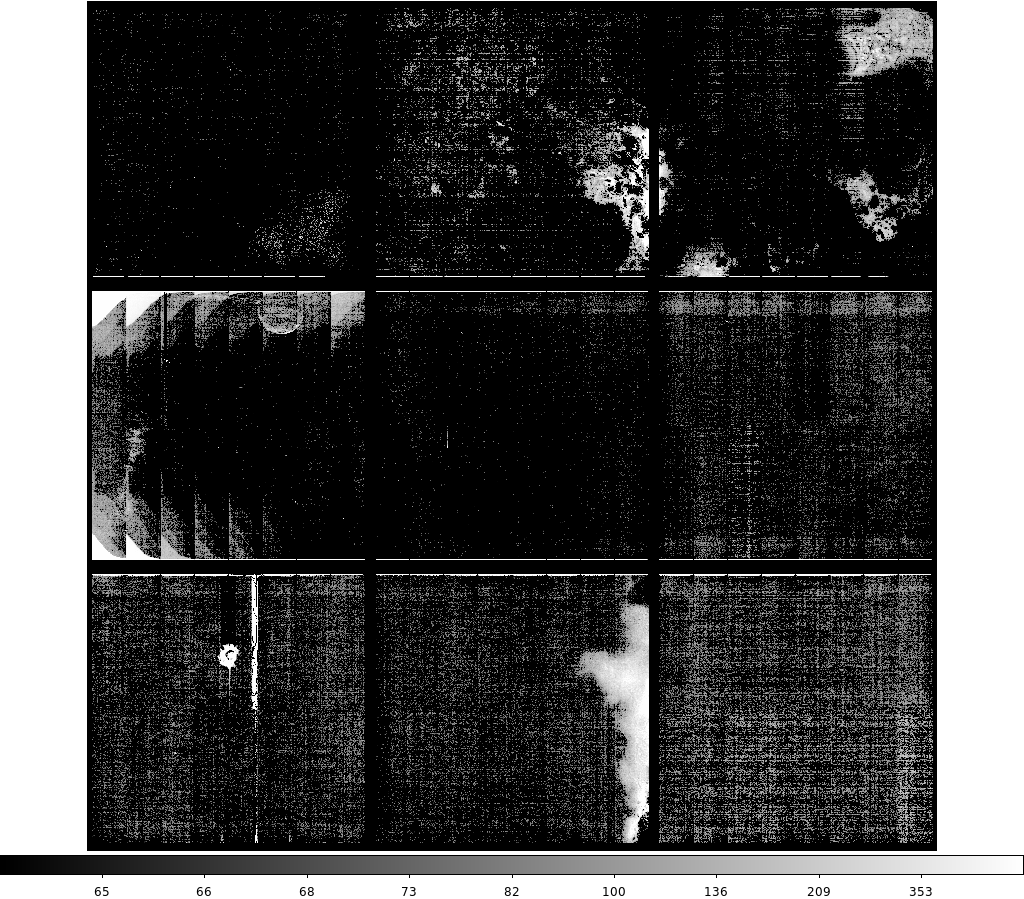
\includegraphics[width=0.9\textwidth]{figures/phosphorescence-survey/itl_fluor_R01_0-19_rb1_log.png}
\caption{Phosphorescence transients for the R01 RTM captured in the first 15\,s following {\it red} CCOB LED at 400\,ke$^-$/pix. With 8$\times$8 blocking, the upper end of the color scale (640) corresponds to 10 e$^-$/pixel when averaged over 64 pixels contributing.}
\label{fig:phos:R01}
\end{figure}

\begin{figure}[!htbp]
\centering
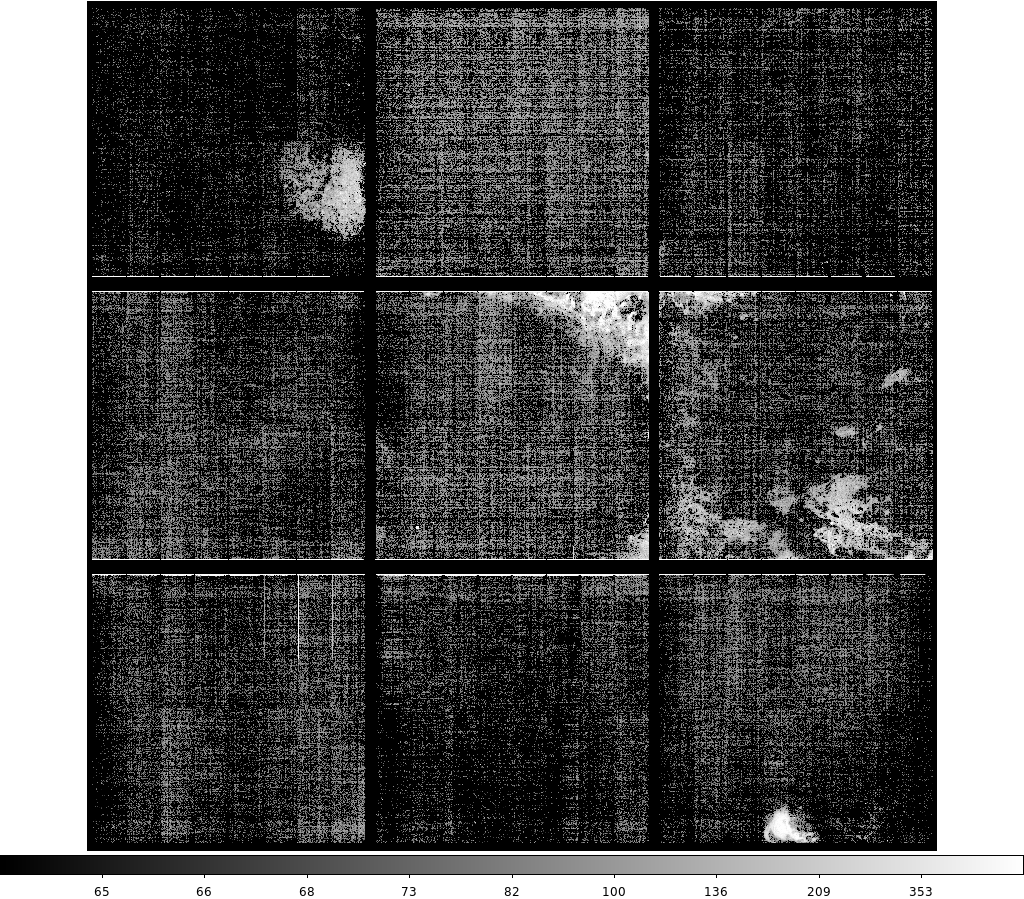
\includegraphics[width=0.9\textwidth]{figures/phosphorescence-survey/itl_fluor_R02_0-19_rb1_log.png}
\caption{Phosphorescence transients for the R02 RTM captured in the first 15\,s following {\it red} CCOB LED at 400\,ke$^-$/pix. With 8$\times$8 blocking, the upper end of the color scale (640) corresponds to 10 e$^-$/pixel when averaged over 64 pixels contributing.}
\label{fig:phos:R02}
\end{figure}

\begin{figure}[!htbp]
\centering
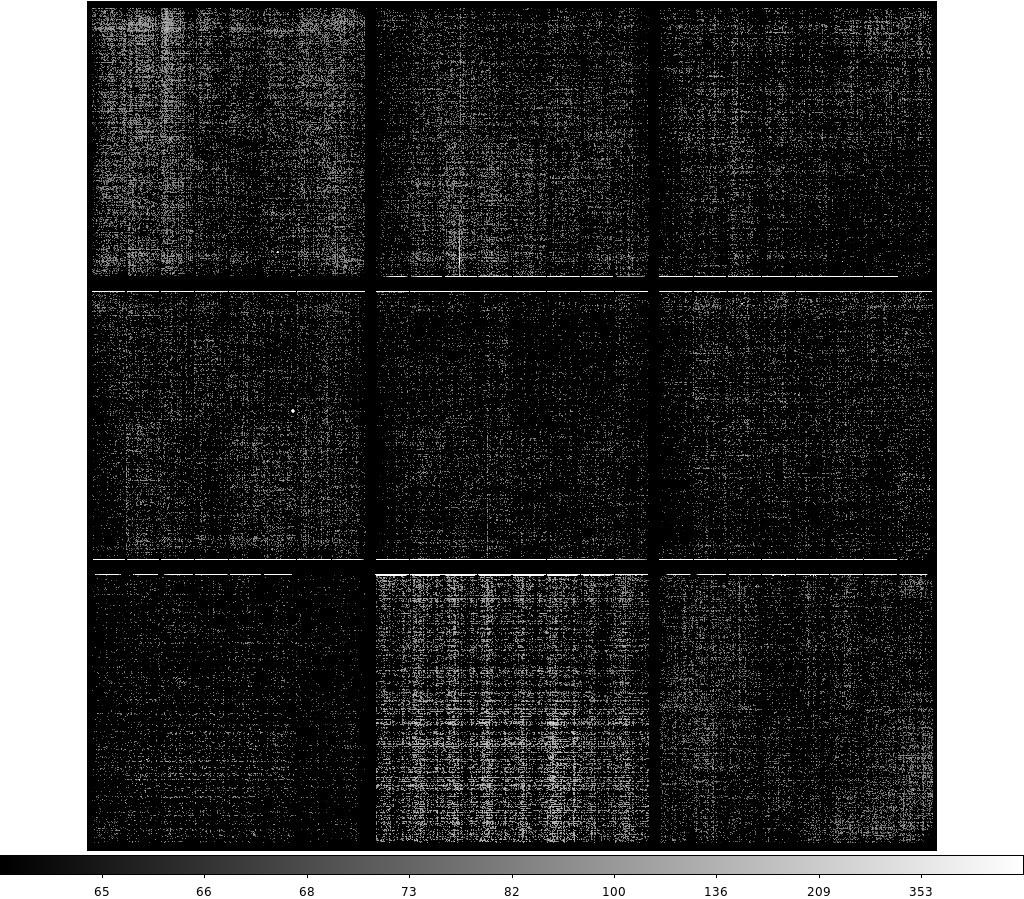
\includegraphics[width=0.9\textwidth]{figures/phosphorescence-survey/itl_fluor_R03_0-19_rb1_log.png}
\caption{Phosphorescence transients for the R03 RTM captured in the first 15\,s following {\it red} CCOB LED at 400\,ke$^-$/pix. With 8$\times$8 blocking, the upper end of the color scale (640) corresponds to 10 e$^-$/pixel when averaged over 64 pixels contributing.}
\label{fig:phos:R03}
\end{figure}

\begin{figure}[!htbp]
\centering
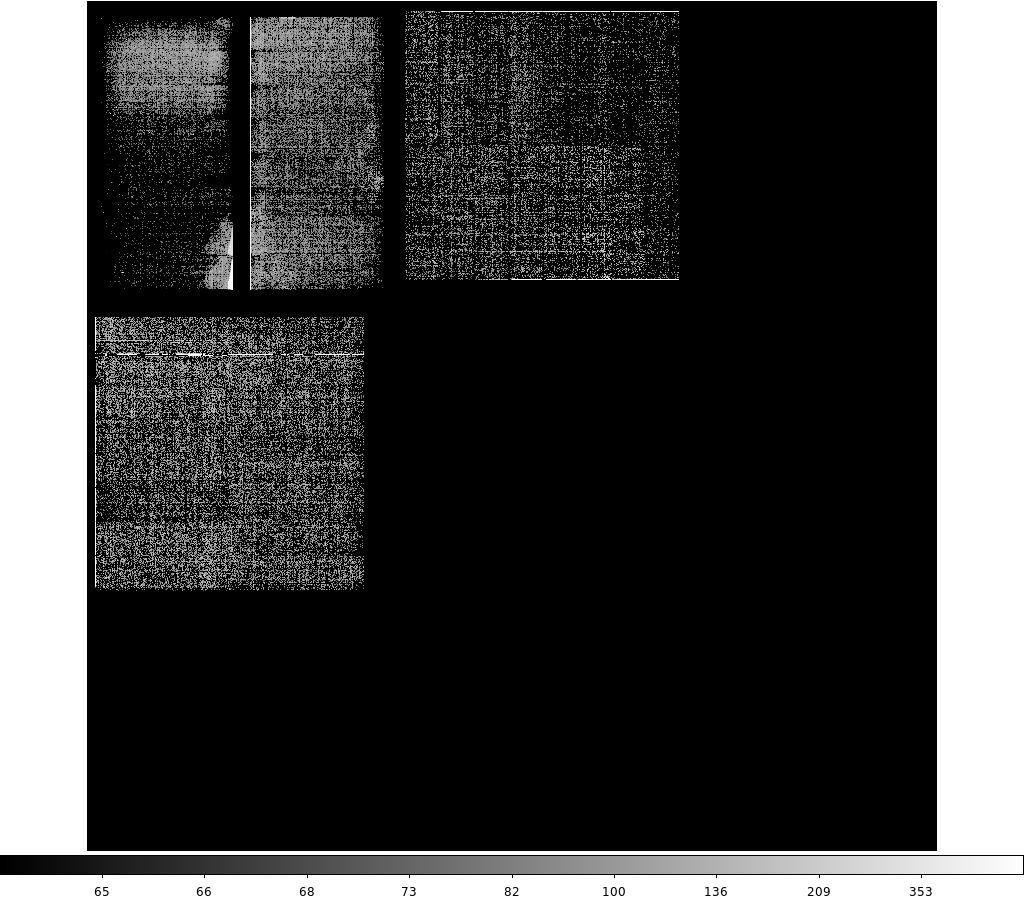
\includegraphics[width=0.9\textwidth]{figures/phosphorescence-survey/itl_fluor_R04_0-19_rb1_log.png}
\caption{Phosphorescence transients for the R04 CRTM captured in the first 15\,s following {\it red} CCOB LED at 400\,ke$^-$/pix. With 8$\times$8 blocking, the upper end of the color scale (640) corresponds to 10 e$^-$/pixel when averaged over 64 pixels contributing.}
\label{fig:phos:R04}
\end{figure}

\begin{figure}[!htbp]
\centering
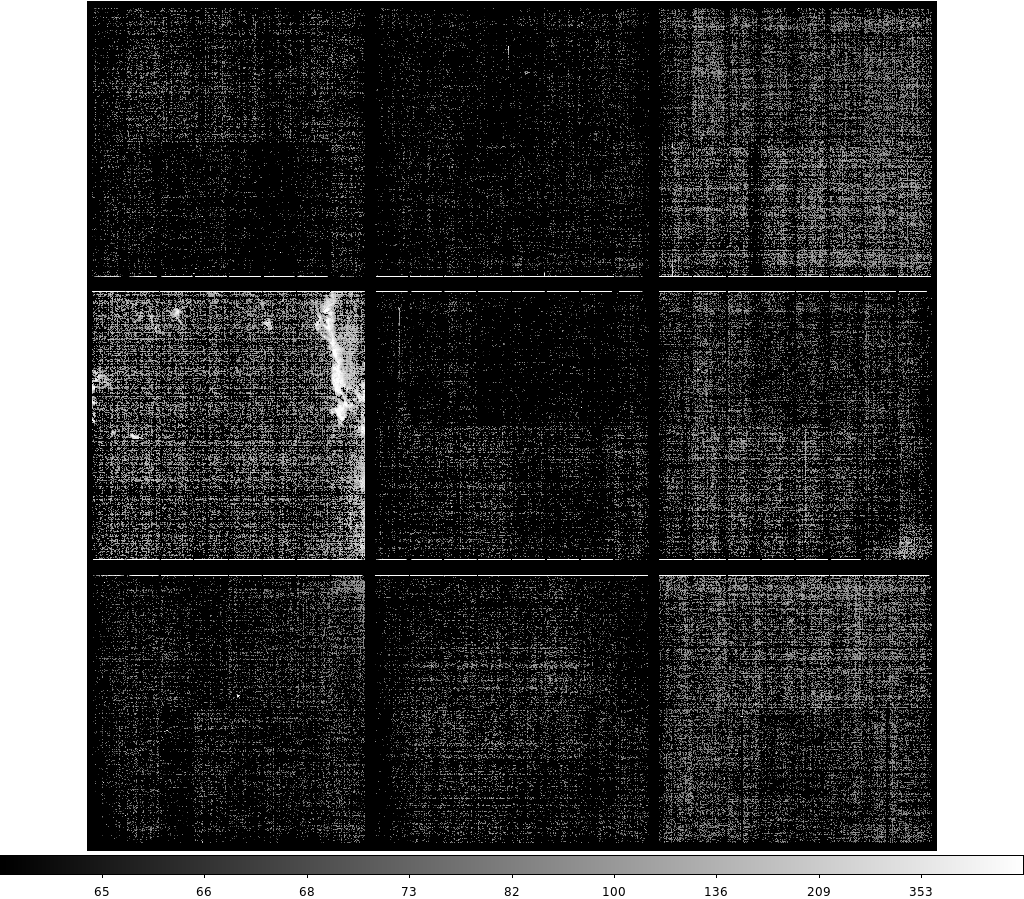
\includegraphics[width=0.9\textwidth]{figures/phosphorescence-survey/itl_fluor_R10_0-19_rb1_log.png}
\caption{Phosphorescence transients for the R10 RTM captured in the first 15\,s following {\it red} CCOB LED at 400\,ke$^-$. With 8$\times$8 blocking, the upper end of the color scale (640) corresponds to 10 e$^-$/pixel when averaged over 64 pixels contributing.}
\label{fig:phos:R10}
\end{figure}

\begin{figure}[!htbp]
\centering
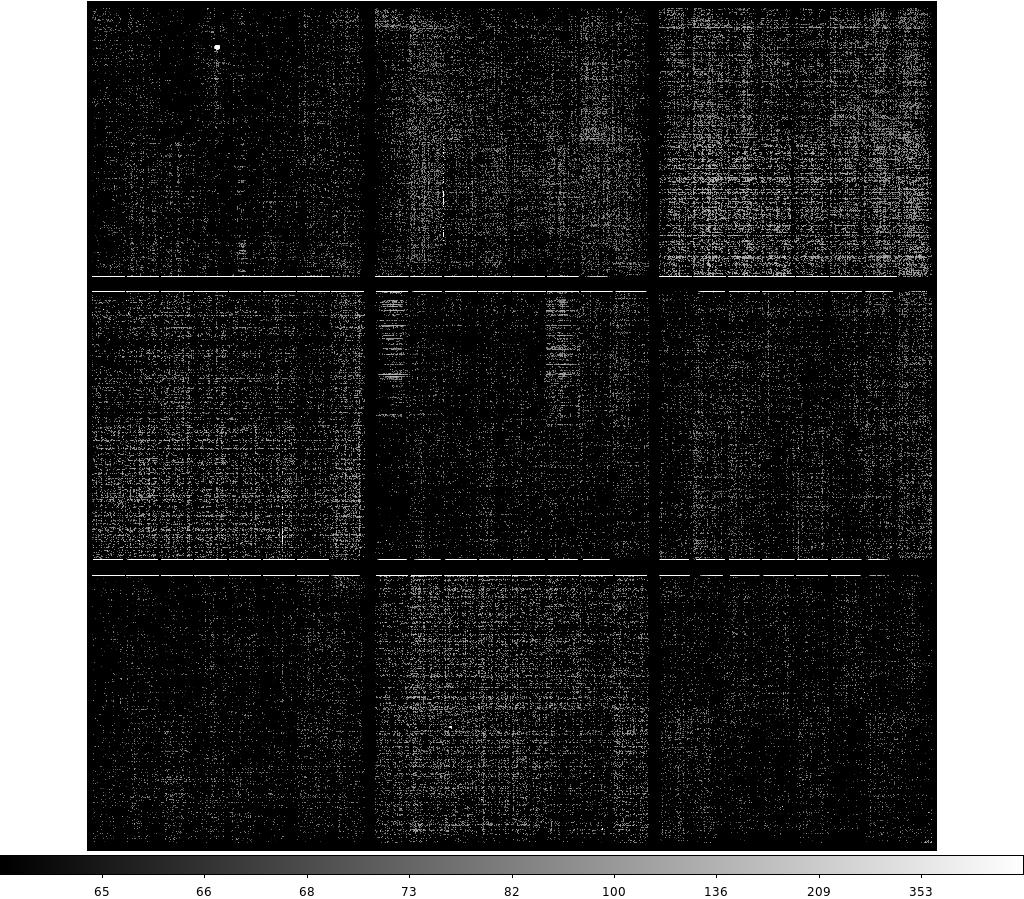
\includegraphics[width=0.9\textwidth]{figures/phosphorescence-survey/itl_fluor_R20_0-19_rb1_log.png}
\caption{Phosphorescence transients for the R20 RTM captured in the first 15\,s following {\it red} CCOB LED at 400\,ke$^-$/pix. With 8$\times$8 blocking, the upper end of the color scale (640) corresponds to 10 e$^-$/pixel when averaged over 64 pixels contributing.}
\label{fig:phos:R20}
\end{figure}

\begin{figure}[!htbp]
\centering
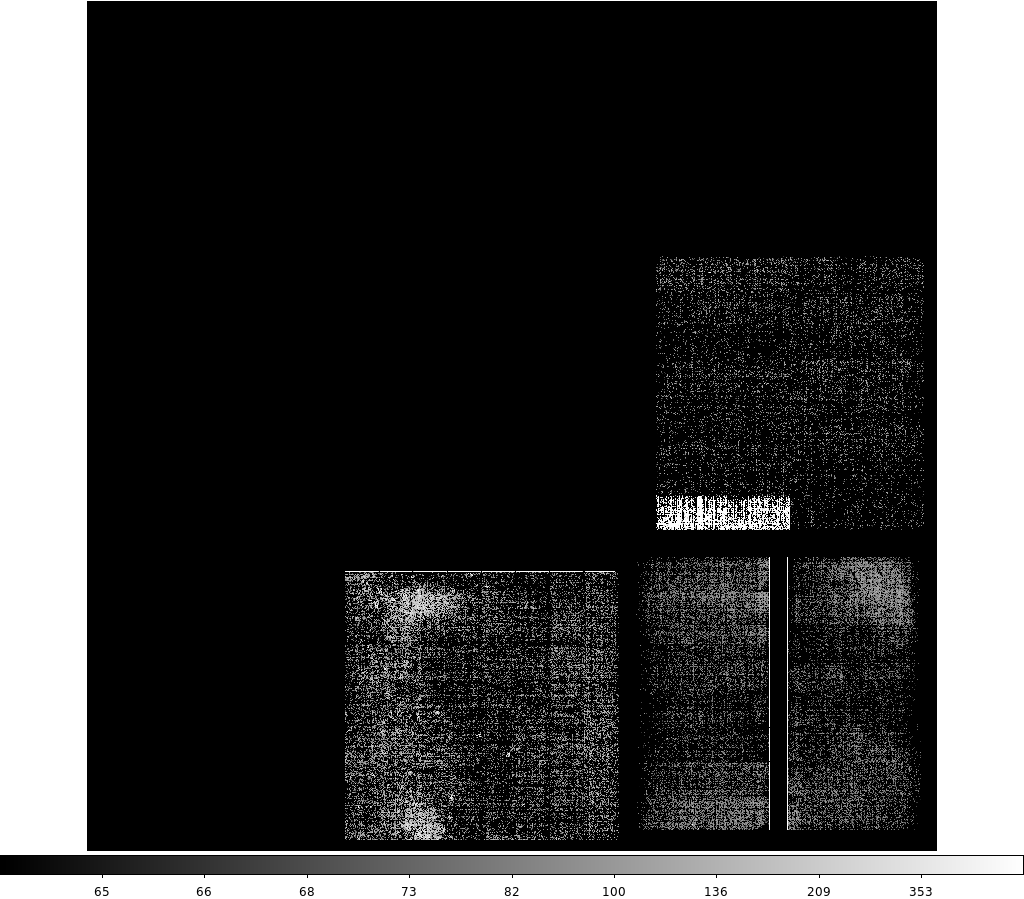
\includegraphics[width=0.9\textwidth]{figures/phosphorescence-survey/itl_fluor_R40_0-19_rb1_log.png}
\caption{Phosphorescence transients for the R40 CRTM captured in the first 15\,s following {\it red} CCOB LED at 400\,ke$^-$/pix. With 8$\times$8 blocking, the upper end of the color scale (640) corresponds to 10 e$^-$/pixel when averaged over 64 pixels contributing.}
\label{fig:phos:R40}
\end{figure}

\begin{figure}[!htbp]
\centering
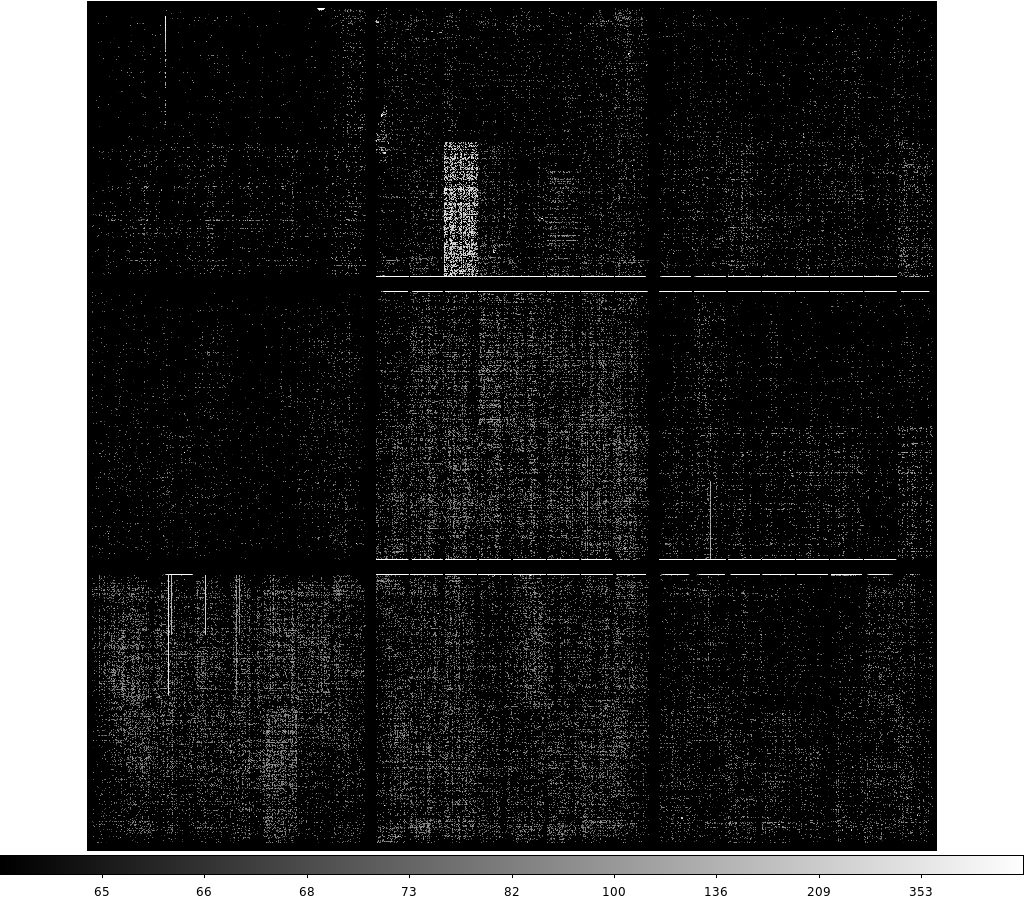
\includegraphics[width=0.9\textwidth]{figures/phosphorescence-survey/itl_fluor_R41_0-19_rb1_log.png}
\caption{Phosphorescence transients for the R41 RTM captured in the first 15\,s following {\it red} CCOB LED at 400\,ke$^-$/pix. With 8$\times$8 blocking, the upper end of the color scale (640) corresponds to 10 e$^-$/pixel when averaged over 64 pixels contributing.}
\label{fig:phos:R41}
\end{figure}

\begin{figure}[!htbp]
\centering
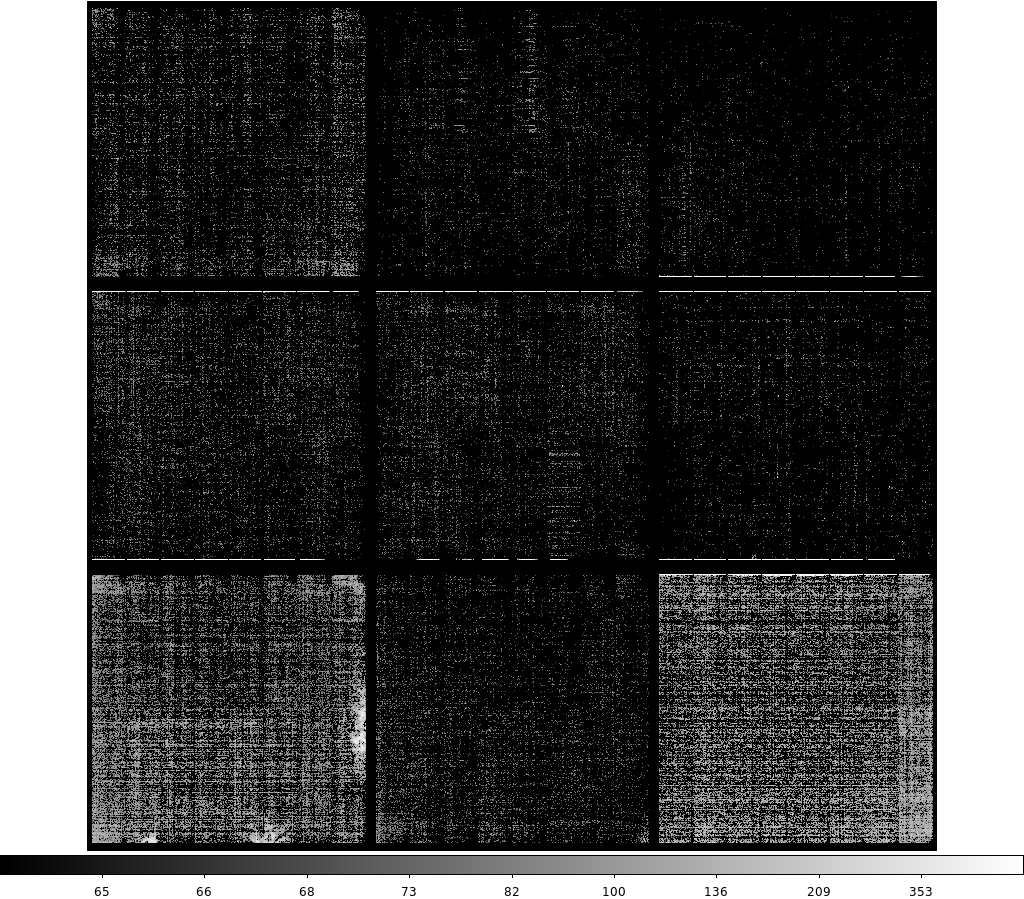
\includegraphics[width=0.9\textwidth]{figures/phosphorescence-survey/itl_fluor_R42_0-19_rb1_log.png}
\caption{Phosphorescence transients for the R42 RTM captured in the first 15\,s following {\it red} CCOB LED at 400\,ke$^-$/pix. With 8$\times$8 blocking, the upper end of the color scale (640) corresponds to 10 e$^-$/pixel when averaged over 64 pixels contributing.}
\label{fig:phos:R42}
\end{figure}

\begin{figure}[!htbp]
\centering
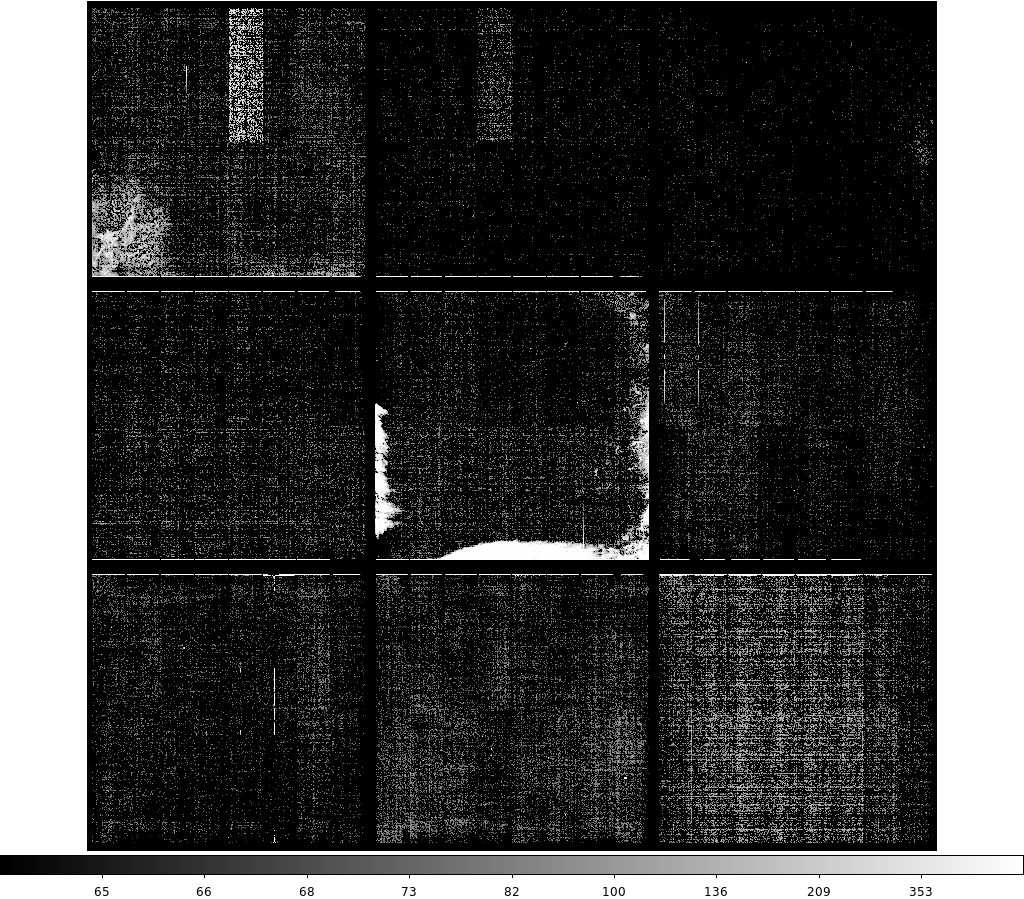
\includegraphics[width=0.9\textwidth]{figures/phosphorescence-survey/itl_fluor_R43_0-19_rb1_log.png}
\caption{Phosphorescence transients for the R43 RTM captured in the first 15\,s following {\it red} CCOB LED at 400\,ke$^-$/pix. With 8$\times$8 blocking, the upper end of the color scale (640) corresponds to 10 e$^-$/pixel when averaged over 64 pixels contributing.}
\label{fig:phos:R43}
\end{figure}

\begin{figure}[!htbp]
\centering
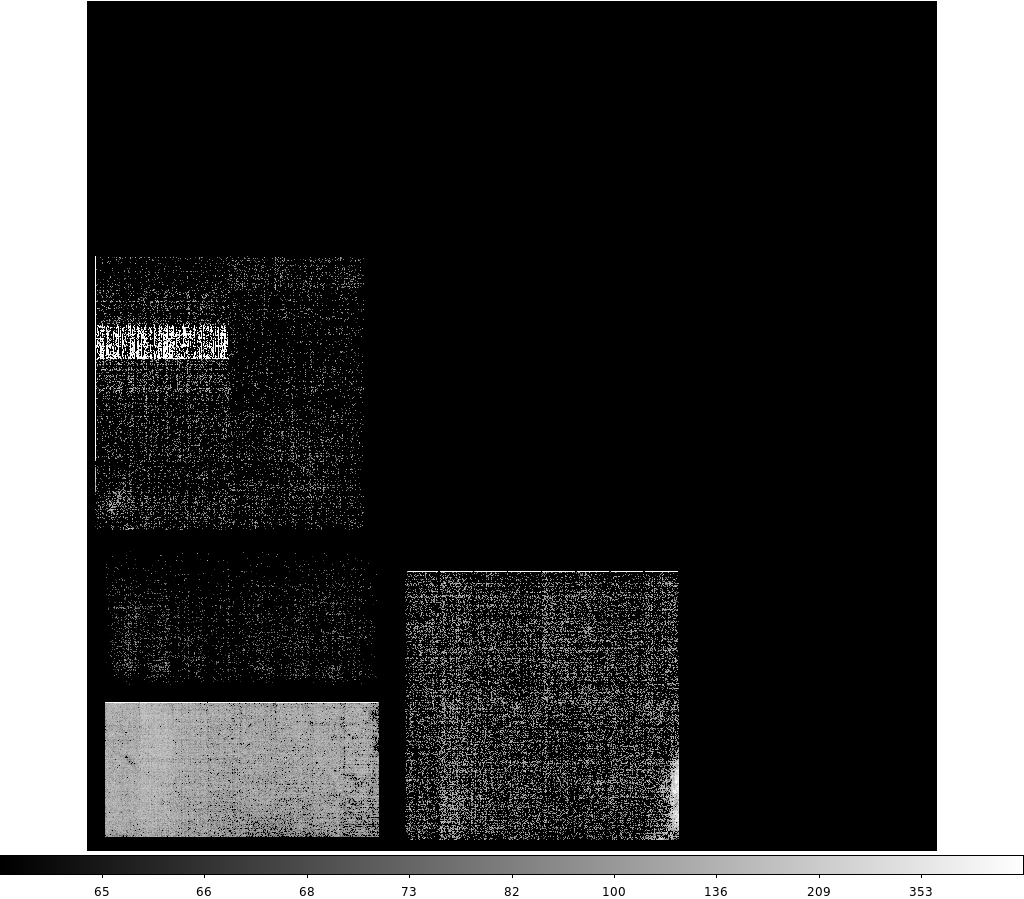
\includegraphics[width=0.9\textwidth]{figures/phosphorescence-survey/itl_fluor_R44_0-19_rb1_log.png}
\caption{Phosphorescence transients for the R44 CRTM captured in the first 15\,s following {\it red} CCOB LED at 400\,ke$^-$/pix. With 8$\times$8 blocking, the upper end of the color scale (640) corresponds to 10 e$^-$/pixel when averaged over 64 pixels contributing.}
\label{fig:phos:R44}
\end{figure}

\clearpage
\section{Phosphorescence morphological comparisons with features seen in {\it blue} flat field response}

The following images (Figures~\ref{fig:phos:stains:R01S00} through \ref{fig:phos:stains:R43S20}) are an incomplete selection of ITL sensors with phosphorescence. They compare expressed phosphorescence (transient term) with the {\it blue} CCOB LED flat response.

\begin{figure}[!htbp]
\centering
\begin{minipage}{1.0\textwidth}    
  \centering
  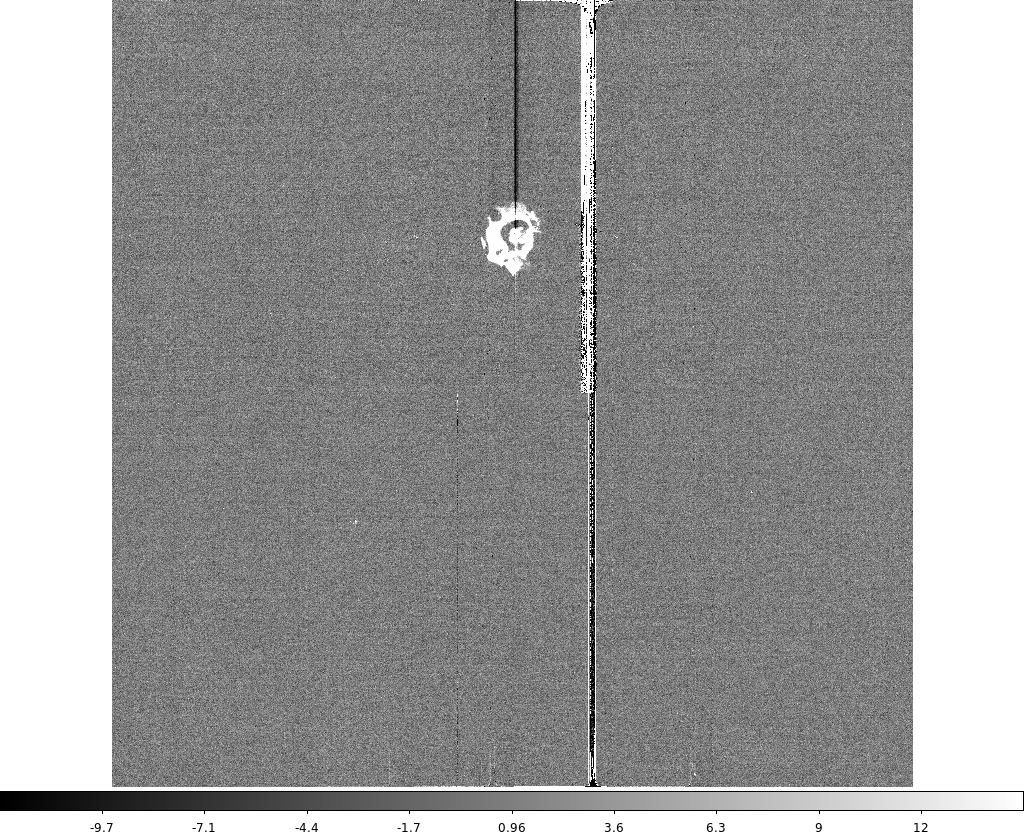
\includegraphics[width=.6\linewidth]{figures/phosphorescence-survey/stains_phos_R01_S00.png}    
\end{minipage}
\begin{minipage}{1.0\textwidth}
  \centering
  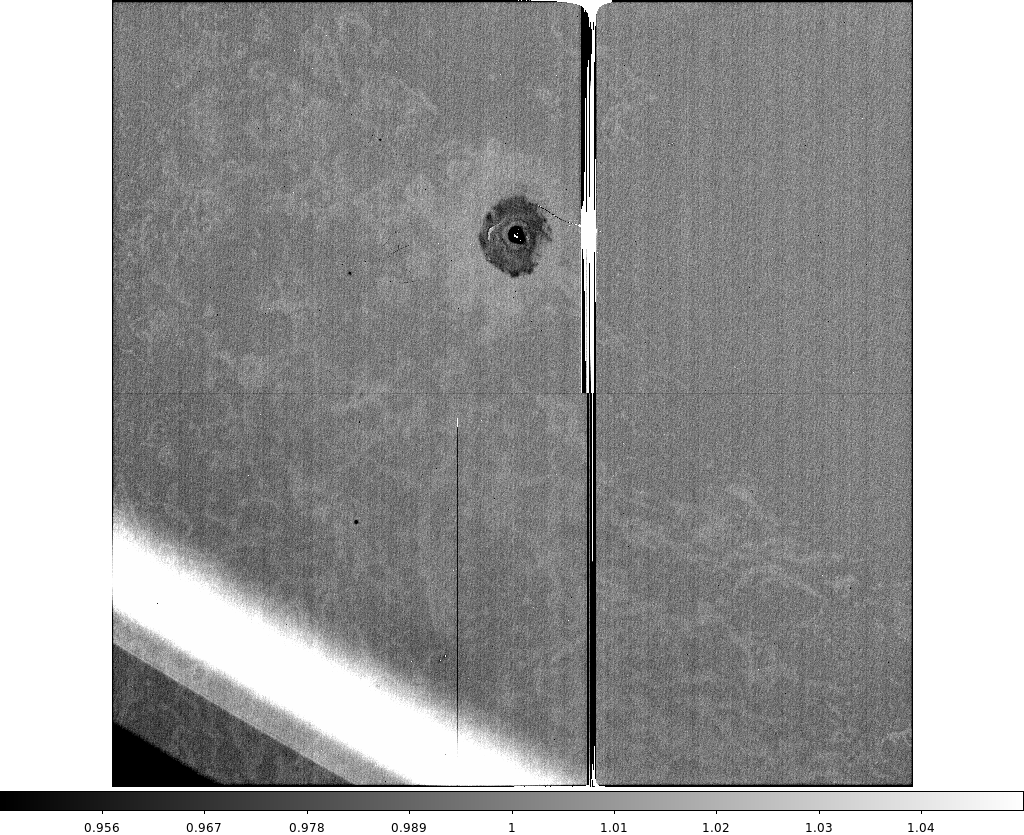
\includegraphics[width=.6\linewidth]{figures/phosphorescence-survey/stains_abs_R01_S00.png}
\end{minipage}
\caption{The ITL sensor R01\_S00. Top: the transient phosphorescence term. Bottom: the {\it blue} flat response. The large, extended spot appears to be centered on a {\it vampire pixel}, which also expresses a large amplitude of phosphorescence, which emits enough current to contaminate the parallel overscan in at least the first 15\,s exposure following trigger. The flat response feature has opposite polarity from the phosphorescence.}
\label{fig:phos:stains:R01S00}
\end{figure}


\begin{figure}[!htbp]
\centering
\begin{minipage}{1.0\textwidth}    
  \centering
  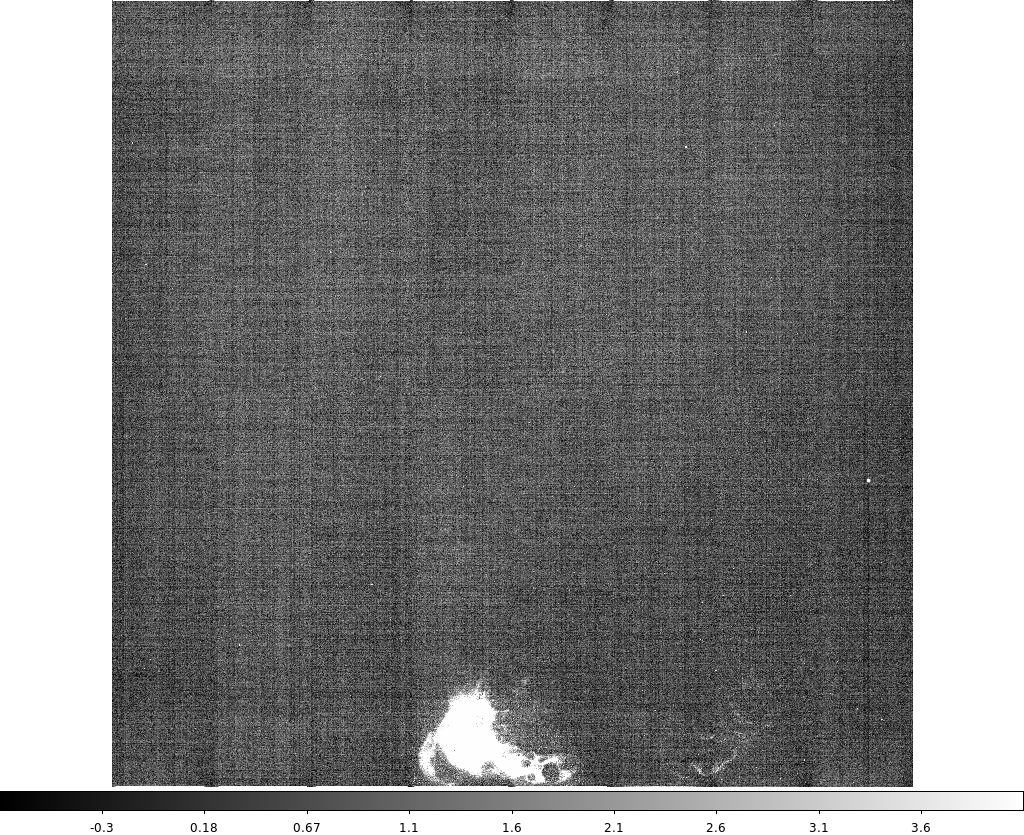
\includegraphics[width=.6\linewidth]{figures/phosphorescence-survey/stains_phos_R02_S02.png}    
\end{minipage}
\begin{minipage}{1.0\textwidth}
  \centering
  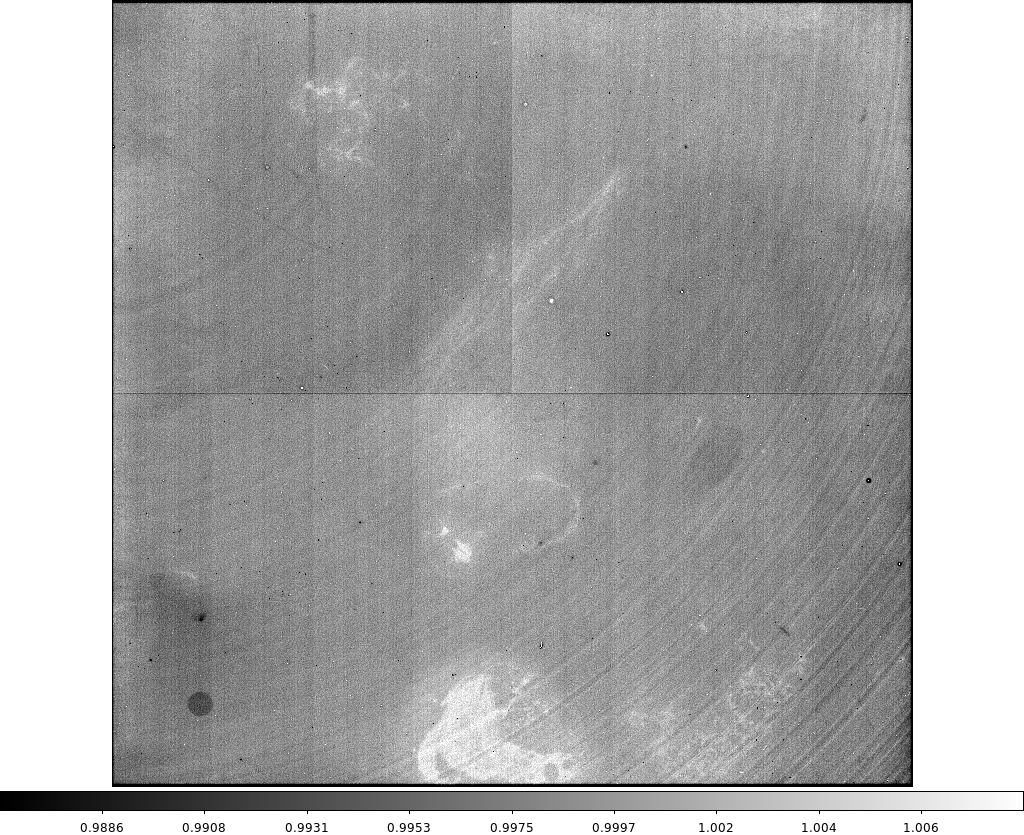
\includegraphics[width=.6\linewidth]{figures/phosphorescence-survey/stains_abs_R02_S02.png}
\end{minipage}
\caption{The ITL sensor R02\_S02. Top: the transient phosphorescence term. Bottom: the {\it blue} flat response. The {\it coffee stain} feature in the flat response has the same polarity as the phosphorescence. A phosphorescent {\it vampire pixel} is seen in segment R02\_S02\_C07.}
\label{fig:phos:stains:R02S02}
\end{figure}

\begin{figure}[!htbp]
\centering
\begin{minipage}{1.0\textwidth}    
  \centering
  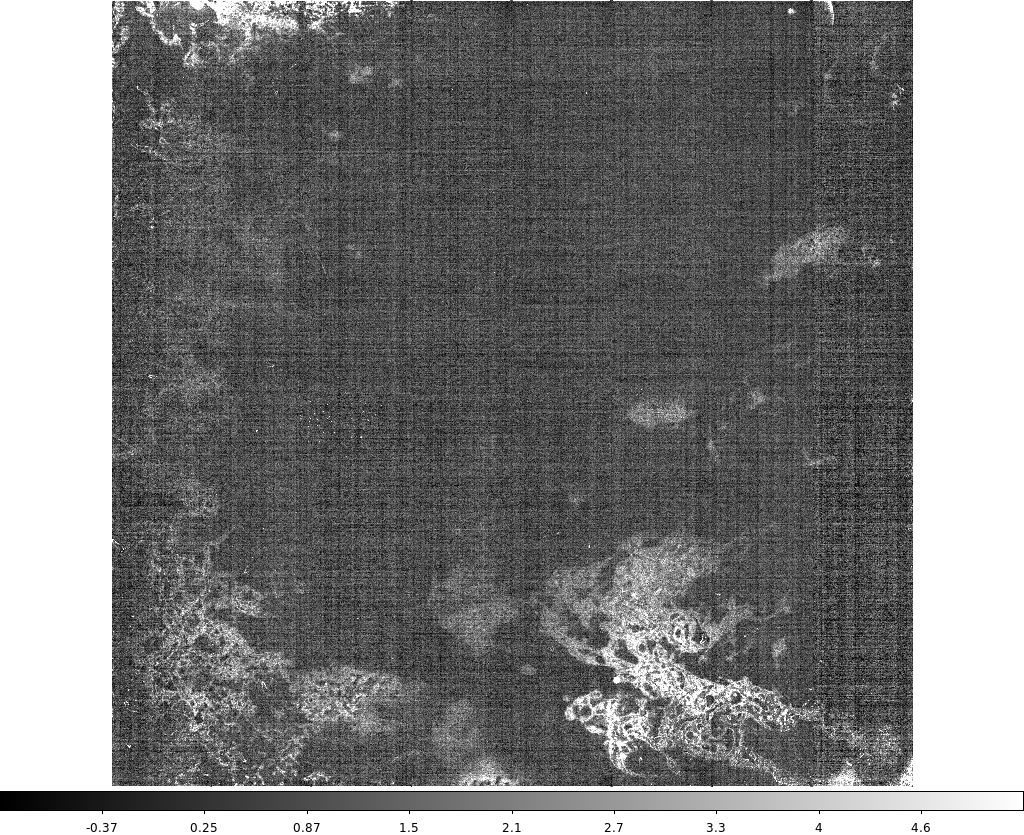
\includegraphics[width=.6\linewidth]{figures/phosphorescence-survey/stains_phos_R02_S12.png}    
\end{minipage}
\begin{minipage}{1.0\textwidth}
  \centering
  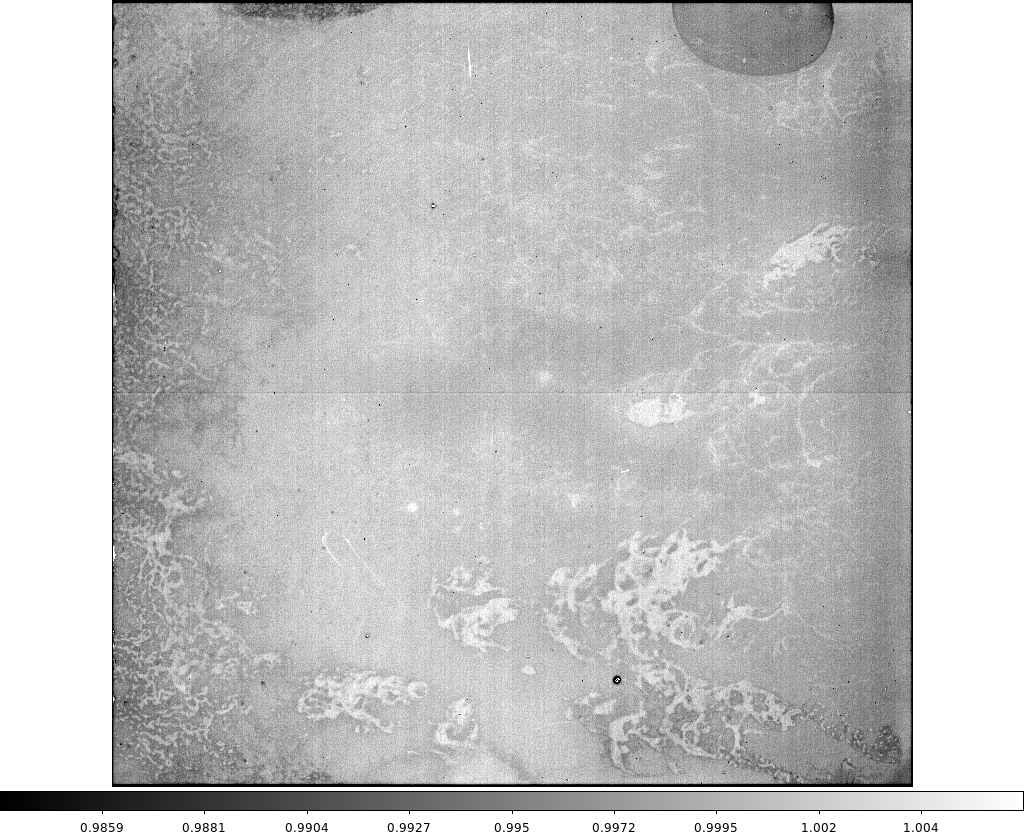
\includegraphics[width=.6\linewidth]{figures/phosphorescence-survey/stains_abs_R02_S12.png}
\end{minipage}
\caption{The ITL sensor R02\_S12. Top: the transient phosphorescence term. Bottom: the {\it blue} flat response. Generally the polarity of the phosphorescence matches that of the {\it coffee stain} in the flat field response, but exceptions include the {\it vampire pixel} seen in segment R02\_S12\_C05.}
\label{fig:phos:stains:R02S12}
\end{figure}


\begin{figure}[!htbp]
\centering
\begin{minipage}{1.0\textwidth}    
  \centering
  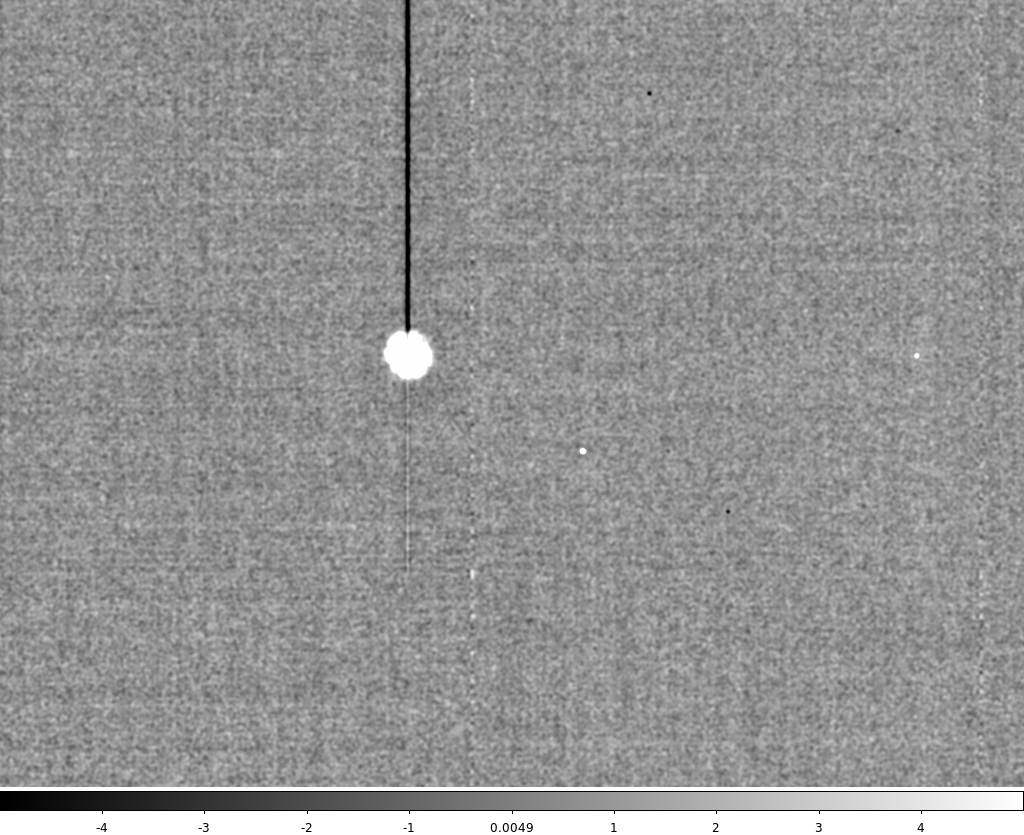
\includegraphics[width=.6\linewidth]{figures/phosphorescence-survey/stains_phos_R03_S10.png}    
\end{minipage}
\begin{minipage}{1.0\textwidth}
  \centering
  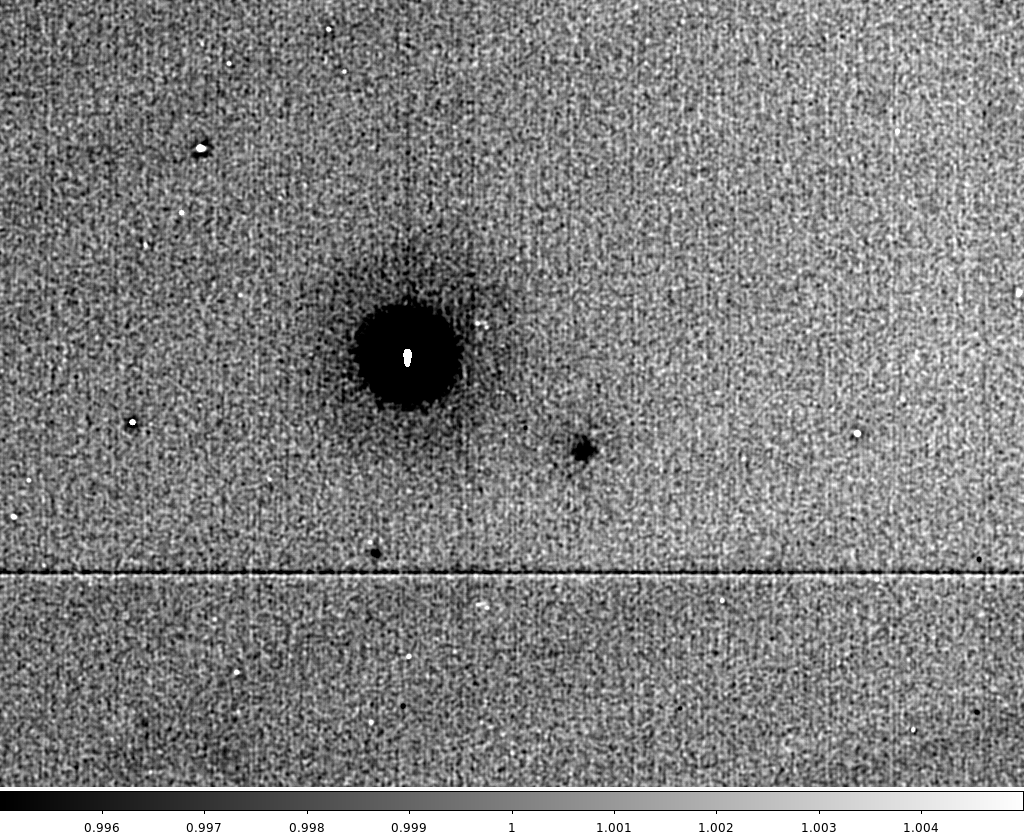
\includegraphics[width=.6\linewidth]{figures/phosphorescence-survey/stains_abs_R03_S10.png}
\end{minipage}
\caption{The ITL sensor R03\_S10, detail of the {\it vampire pixel} of R03\_S10\_C15. Top: the transient phosphorescence term. Bottom: the {\it blue} flat response. As in previous examples, this {\it vampire pixel}'s transient term is large enough to contaminate the parallel overscan even after the first 15\,s following trigger.}
\label{fig:phos:stains:R03S10}
\end{figure}


\begin{figure}[!htbp]
\centering
\begin{minipage}{1.0\textwidth}    
  \centering
  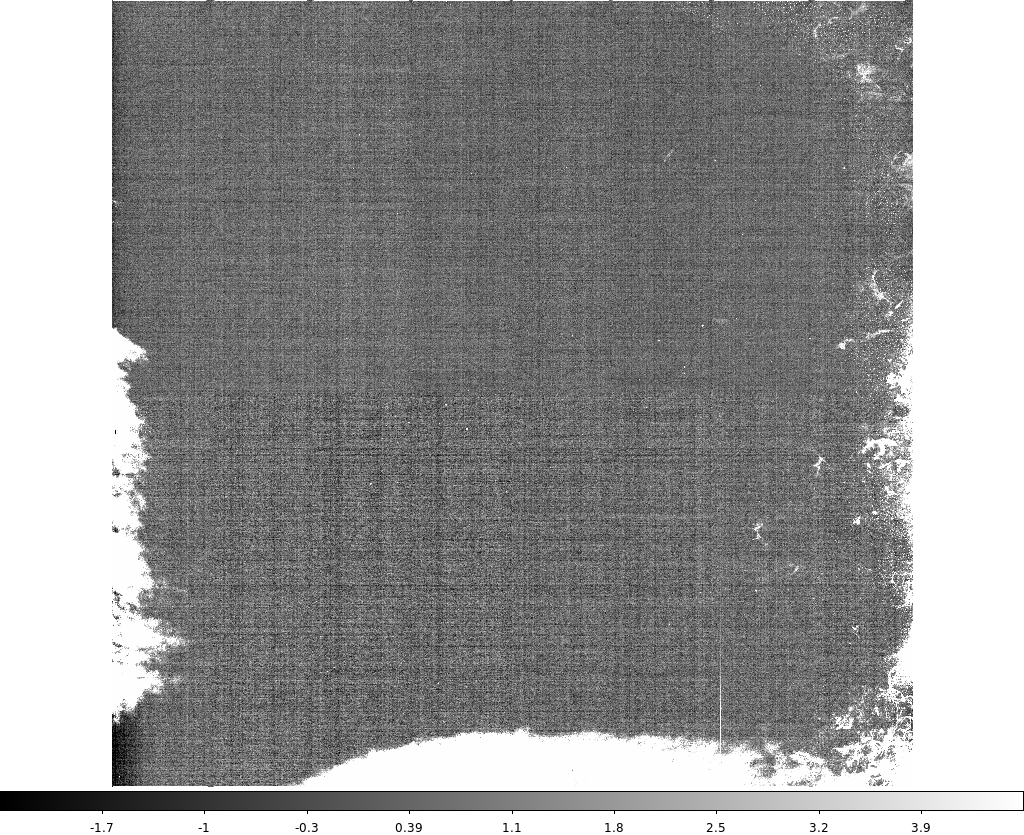
\includegraphics[width=.6\linewidth]{figures/phosphorescence-survey/stains_phos_R43_S11.png}    
\end{minipage}
\begin{minipage}{1.0\textwidth}
  \centering
  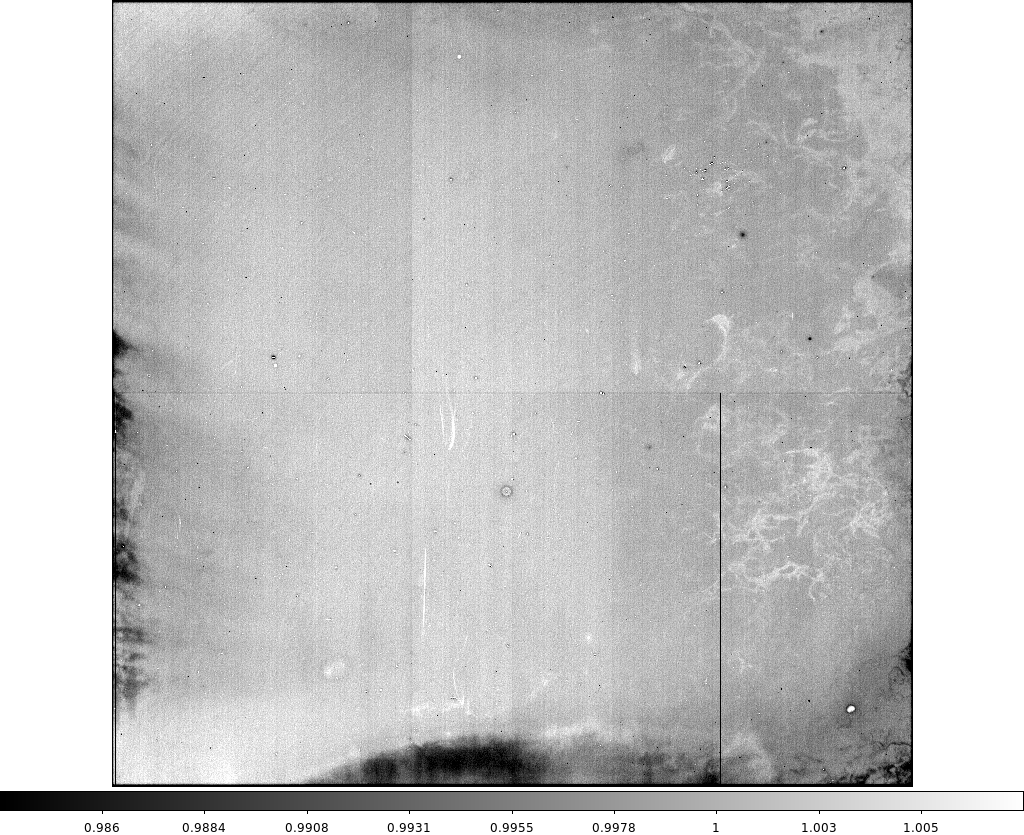
\includegraphics[width=.6\linewidth]{figures/phosphorescence-survey/stains_abs_R43_S11.png}
\end{minipage}
\caption{The ITL sensor R43\_S11. Top: the transient phosphorescence term. Bottom: the {\it blue} flat response. This sensor appears to have the largest integrated phosphorescence among ITL sensors studied. The flat response feature has opposite polarity from the phosphorescence.}
\label{fig:phos:stains:R43S11}
\end{figure}


\begin{figure}[!htbp]
\centering
\begin{minipage}{1.0\textwidth}    
  \centering
  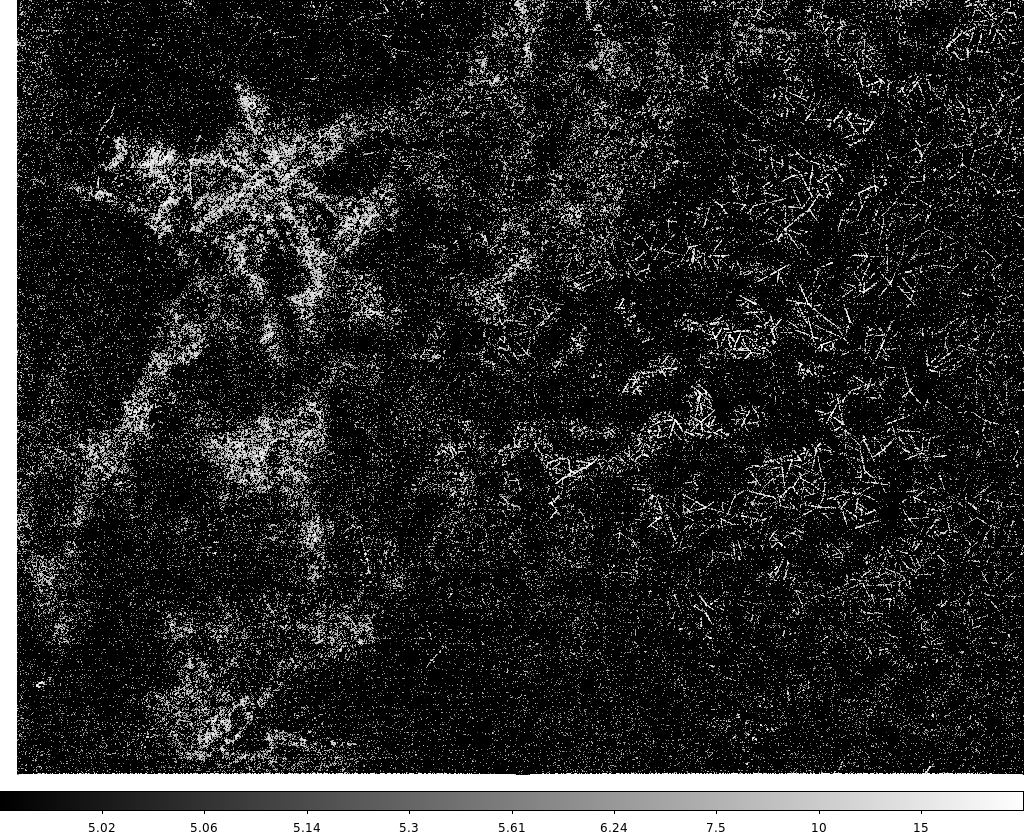
\includegraphics[width=.6\linewidth]{figures/phosphorescence-survey/stains_phos_R43_S20_detail.png}    
\end{minipage}
\begin{minipage}{1.0\textwidth}
  \centering
  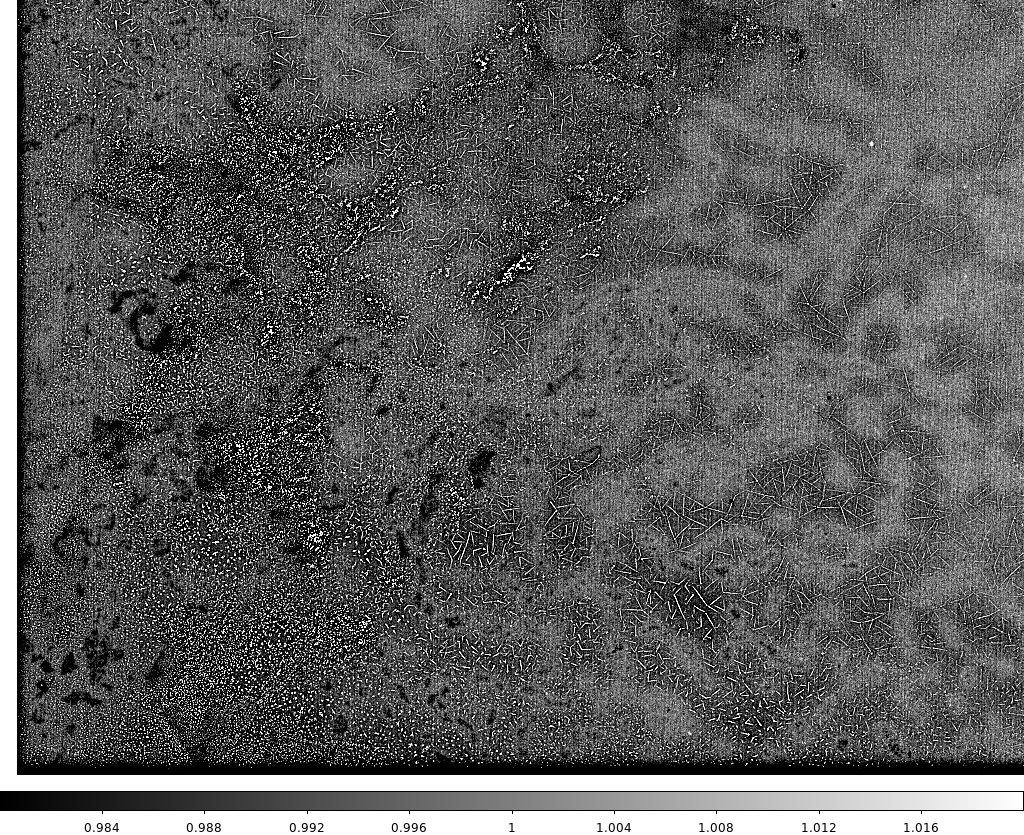
\includegraphics[width=.6\linewidth]{figures/phosphorescence-survey/stains_abs_R43_S20_detail.png}
\end{minipage}
\caption{The ITL sensor R43\_S20, segments C00 through C03. Top: the transient phosphorescence term. Bottom: the {\it blue} flat response. This sensor apparently exhibits peculiar radial crazing patterns seen in both phosphorescence as well as in flat field response, with polarities aligned.}
\label{fig:phos:stains:R43S20}
\end{figure}

\clearpage
\section{Phosphorescence kinetics characterization}
\label{sect:kinetics}
Figures~\ref{fig:phos:kinetics:R01S00} through \ref{fig:phos:kinetics:R43S20} quantify the expressed phosphorescence distributions in ROIs on seven of the problematic ITL sensors. Previously, we had captured the phosphorescence {\it transient term} across the ITL sensors ({\it cf.} Figs.~\ref{fig:phos:R00} thru \ref{fig:phos:R44}); here we track ROI pixel distribution parameters of individual median images constructed from the selection of specific images acquired across the 20 B-protocol datasets available (listed in Table~\ref{tab:phosphorescence:datasets}). 

By fitting decay models to these persistence curves, it is immediately clear that there are multiple (>2) timescales at play for the pixels in each ROI. An example of such a fit is given in Figure~\ref{fig:phos:kinetics:fit:R20S20C13} where a 3-population relaxation model is used to characterize evolution of the 99\% quantile level of the distribution. In this case, there are three different exponential timescales determined: $(\tau_1,\tau_2,\tau_3) = (0.62,2.5,18.3)$ in image units (10.9, 43.8 \& 320 seconds, respectively). The corresponding ratio of these populations works out to 4.5\% (fast), 21.5\% (medium) and 74\% (slow), respectively. Inspection of the more detailed parameters plotted generally indicate skewed distributions from mismatches between medians and means; the choice of the 99\% quantile level to characterize was mainly to estimate the degree to which images would need to be phosphorescence-corrected (and/or the variance plane modified, given the asymmetric impact of the position specific, phosphorescence contribution in recorded images). 

\begin{figure}[!htbp]
\centering
\begin{subfigure}{0.8\textwidth}    
  \centering
  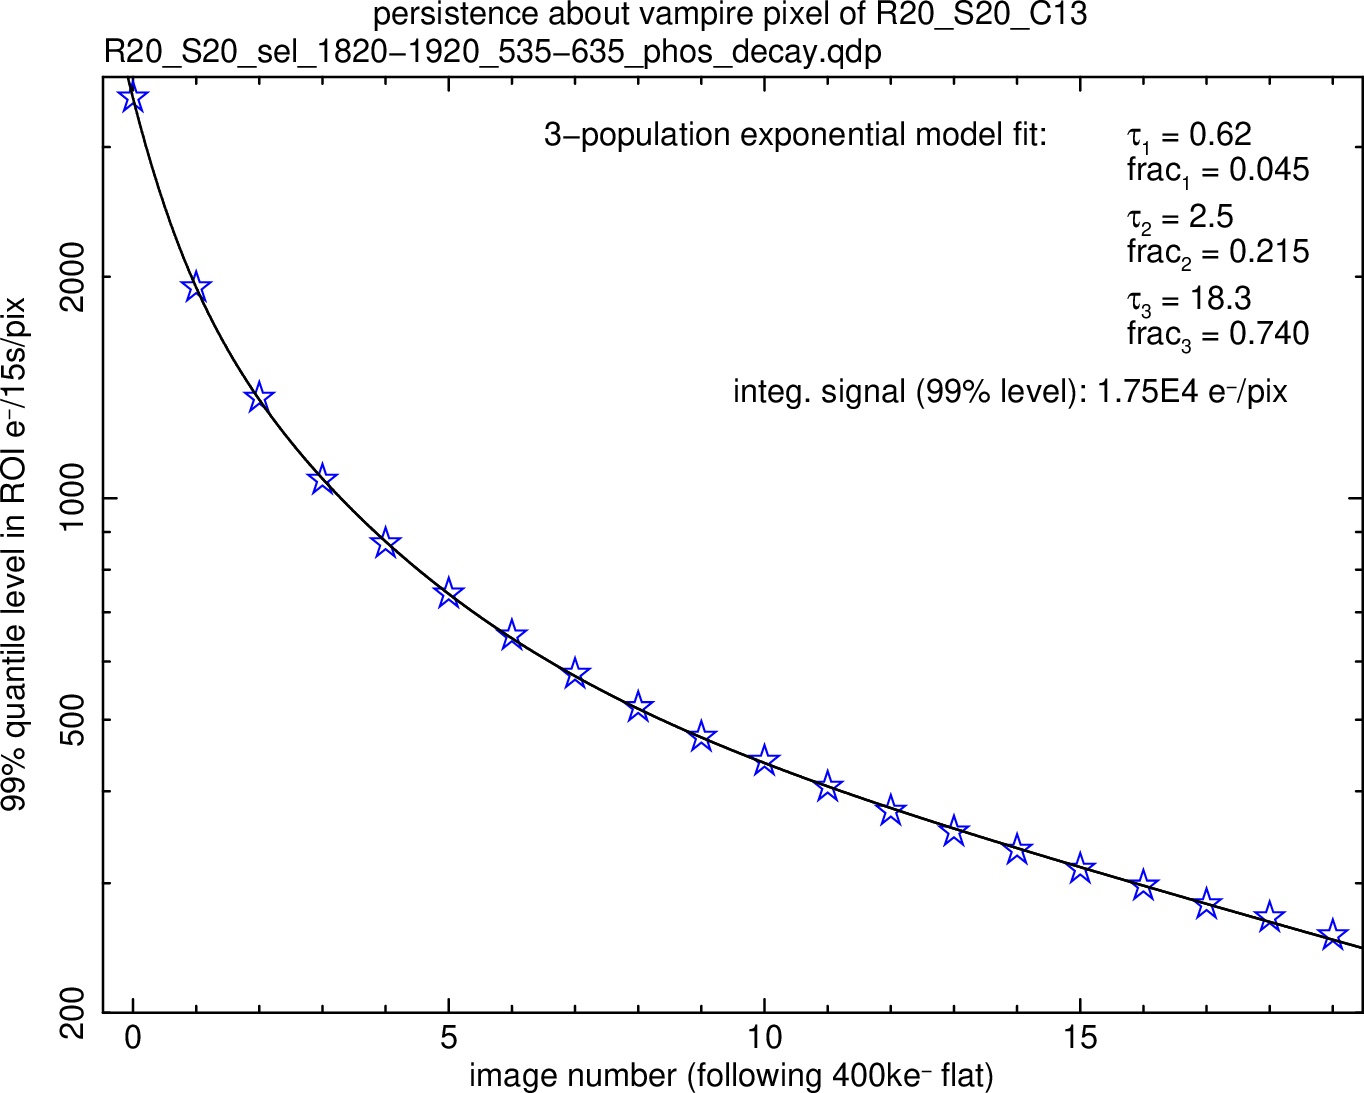
\includegraphics[width=\textwidth]{figures/phosphorescence-survey/phos_kinetics/R20_S20_sel_1820-1920_535-635_phos_decay_fit.png}    
\end{subfigure}
\caption{A three-population fit of the phosphorescence expressed by the vapire pixel region of R20\_S20\_C13. The fit was performed on the 99\% quantile level where signal levels are well above the $3\sigma$ level of the noise distribution. Here, image numbers are parasitically used as time units, with roughly 17.5 seconds per image.}
\label{fig:phos:kinetics:fit:R20S20C13}
\end{figure}

\begin{figure}[!htbp]
\begin{subfigure}{0.45\textwidth}    
  \centering
  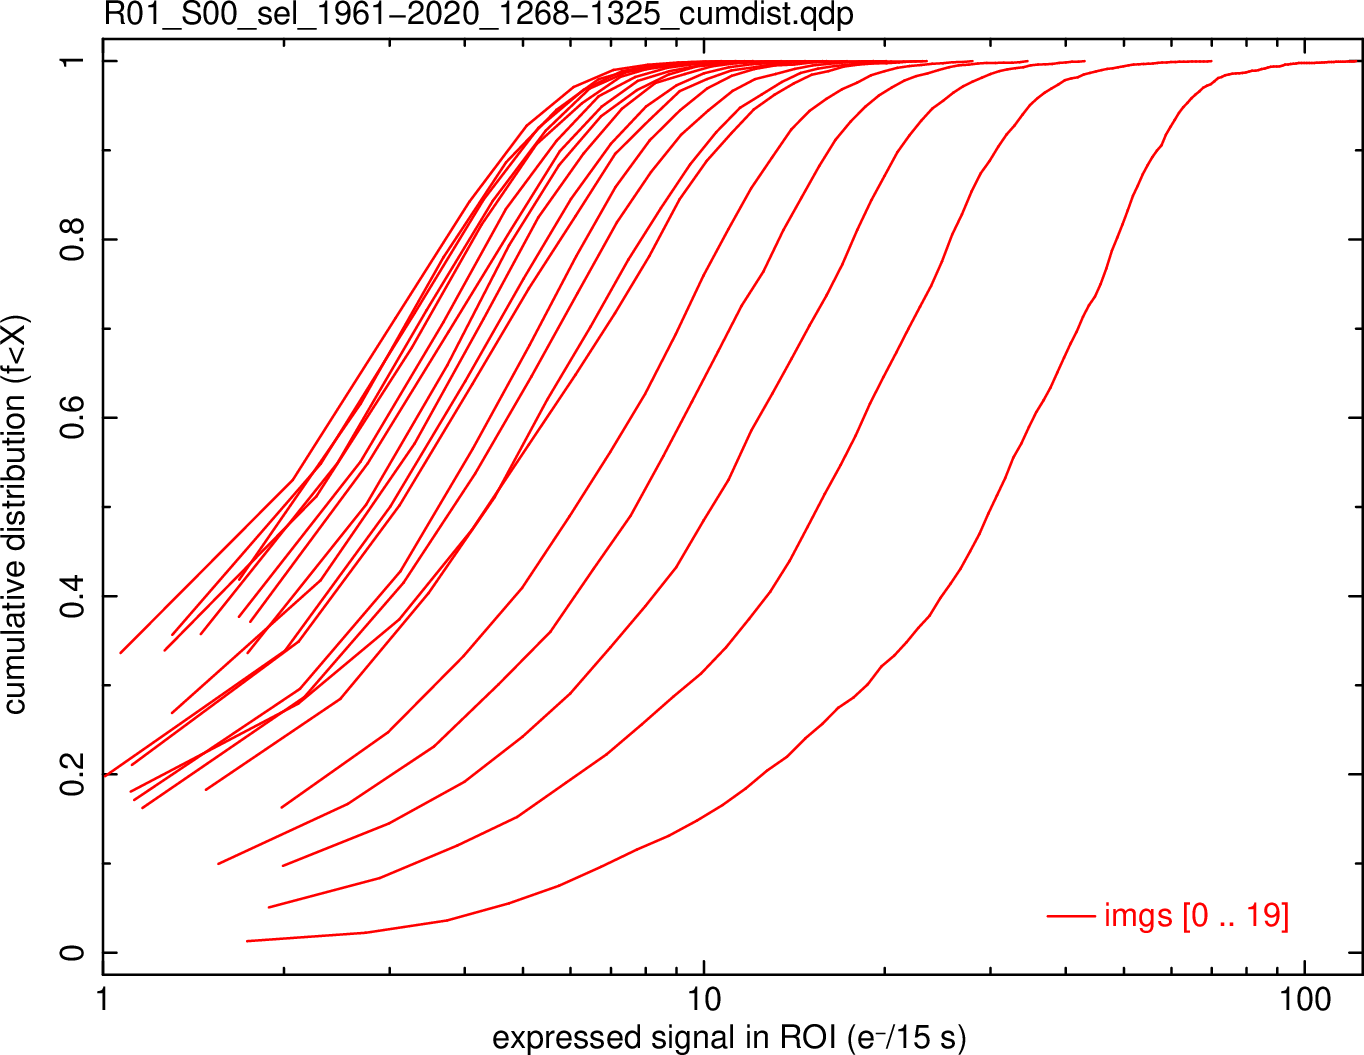
\includegraphics[width=\textwidth]{figures/phosphorescence-survey/phos_kinetics/R01_S00_sel_1961-2020_1268-1325_cumdist.png}    
\end{subfigure}
\hfil
\begin{subfigure}{0.45\textwidth}
  \centering
  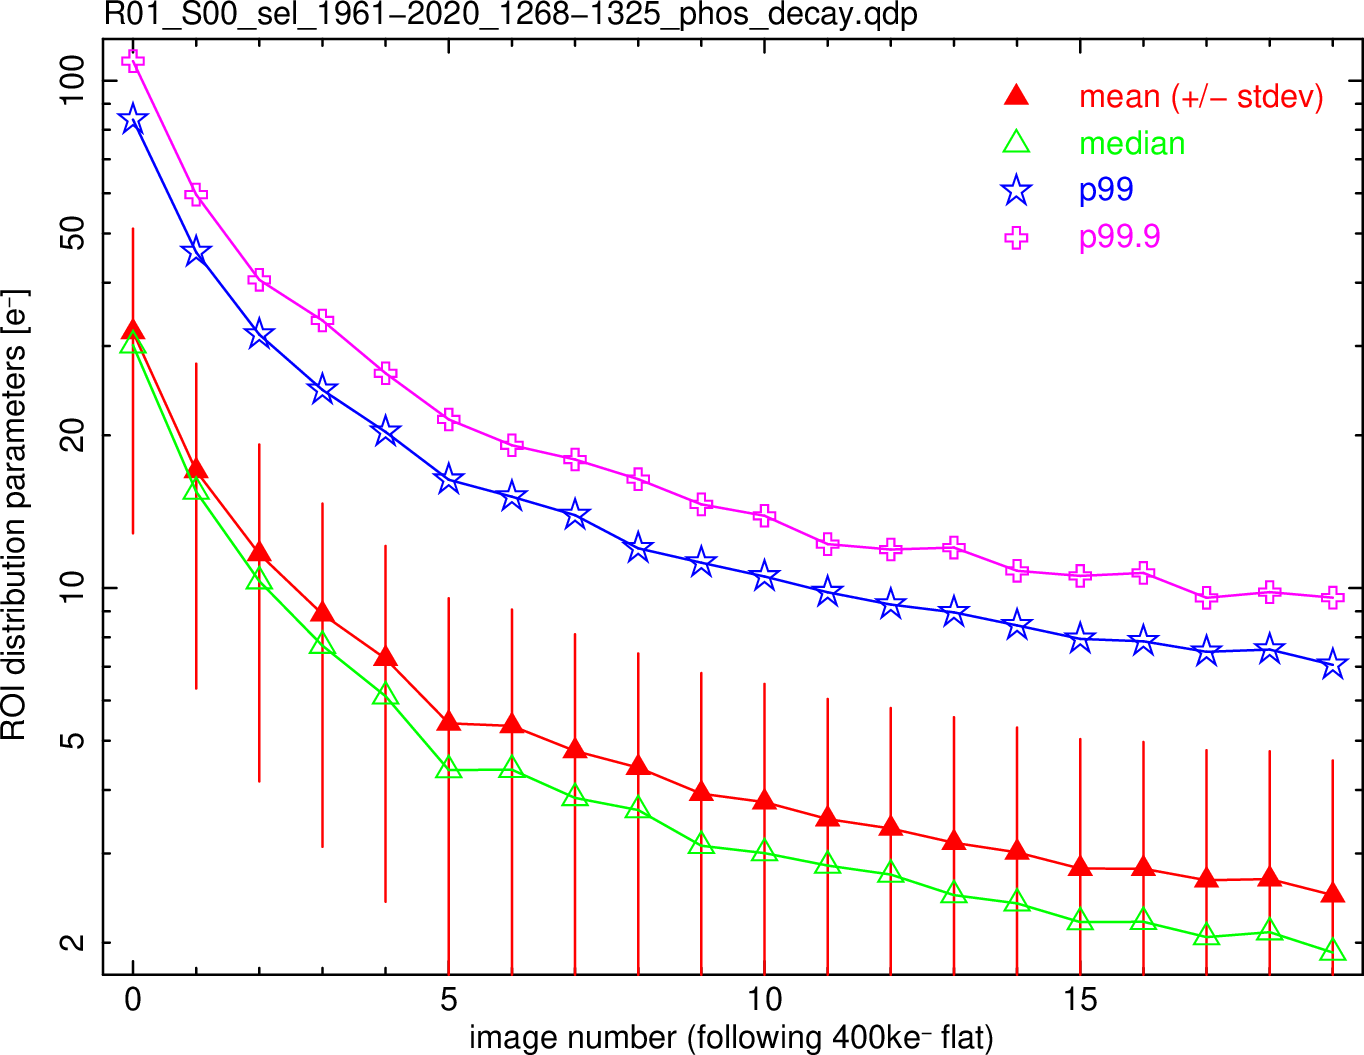
\includegraphics[width=\textwidth]{figures/phosphorescence-survey/phos_kinetics/R01_S00_sel_1961-2020_1268-1325_phos_decay.png}
\end{subfigure}
\newline
\begin{subfigure}{0.45\textwidth}    
  \centering
  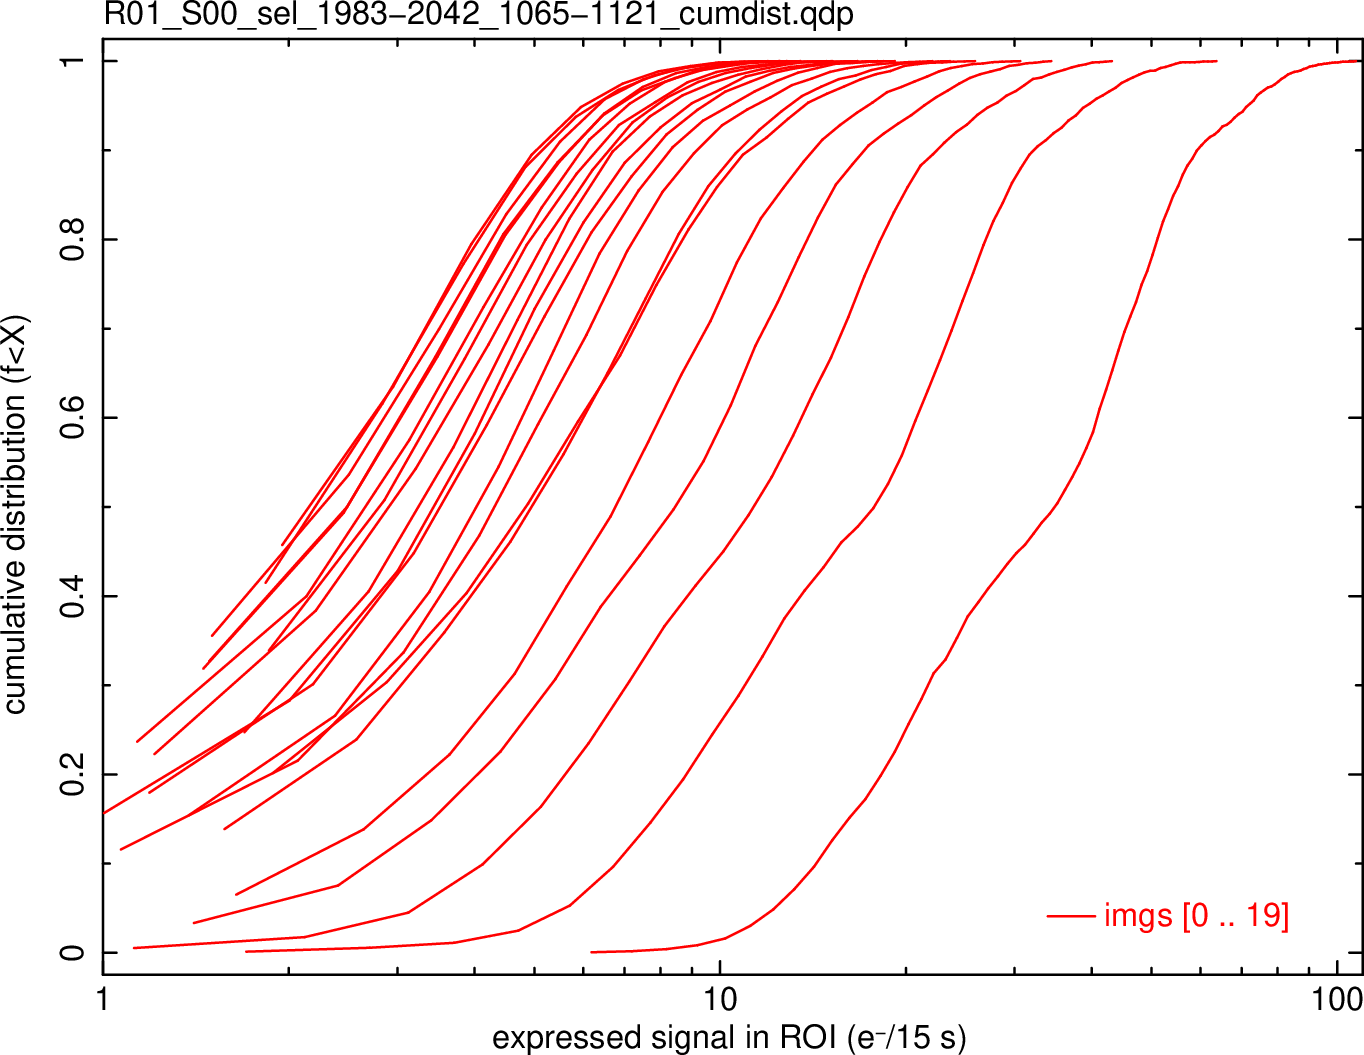
\includegraphics[width=\textwidth]{figures/phosphorescence-survey/phos_kinetics/R01_S00_sel_1983-2042_1065-1121_cumdist.png}    
\end{subfigure}
\hfil
\begin{subfigure}{0.45\textwidth}
  \centering
  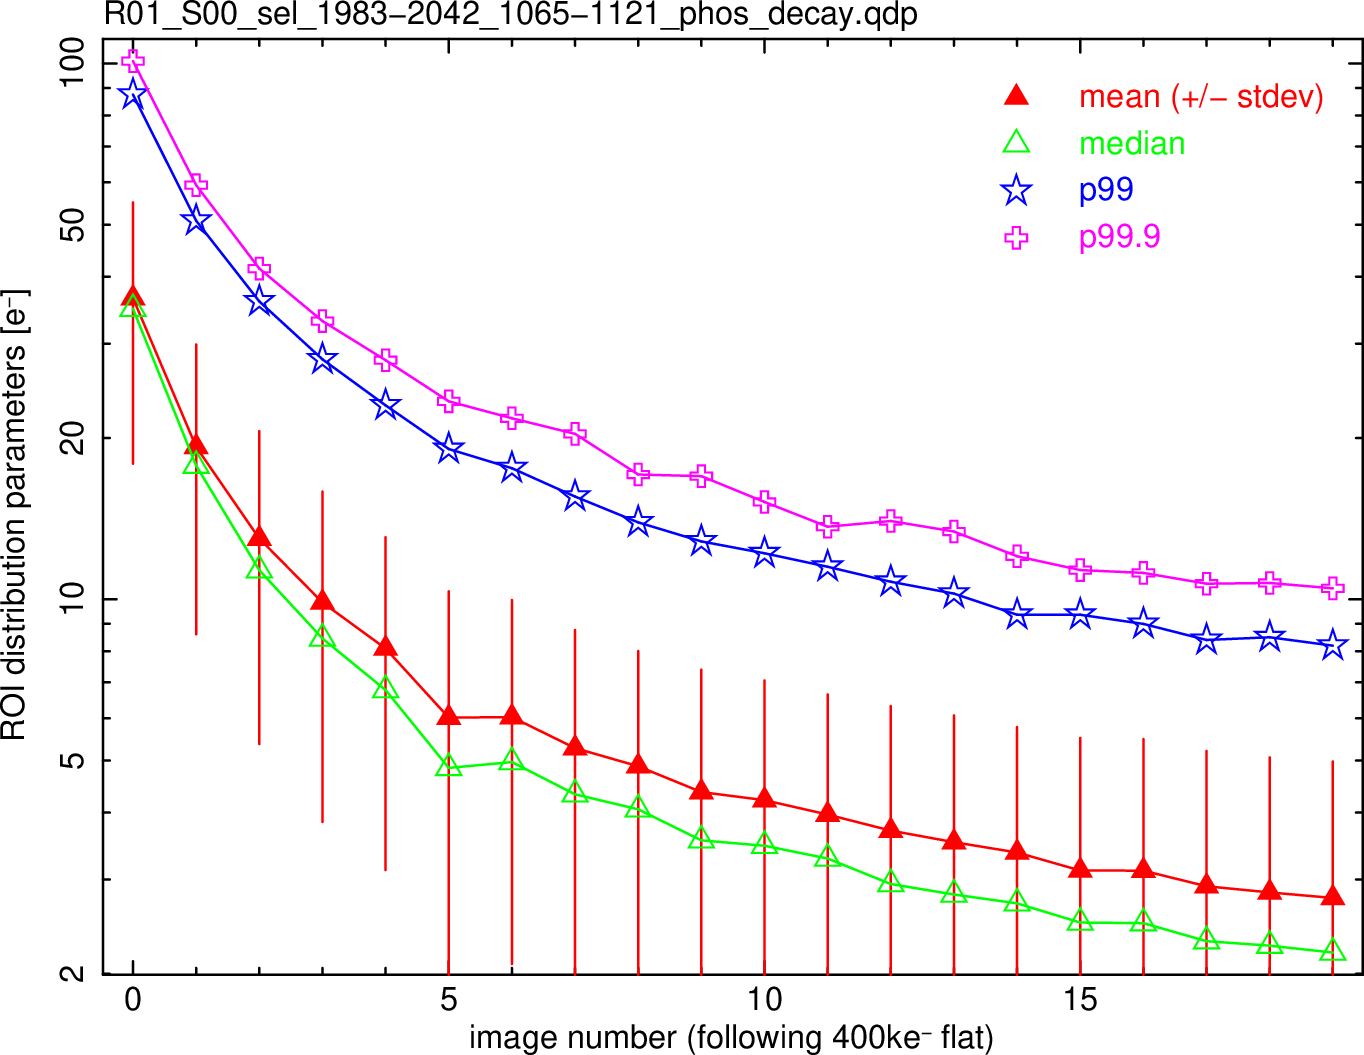
\includegraphics[width=\textwidth]{figures/phosphorescence-survey/phos_kinetics/R01_S00_sel_1983-2042_1065-1121_phos_decay.png}
\end{subfigure}
\newline
\begin{subfigure}{0.45\textwidth}    
  \centering
  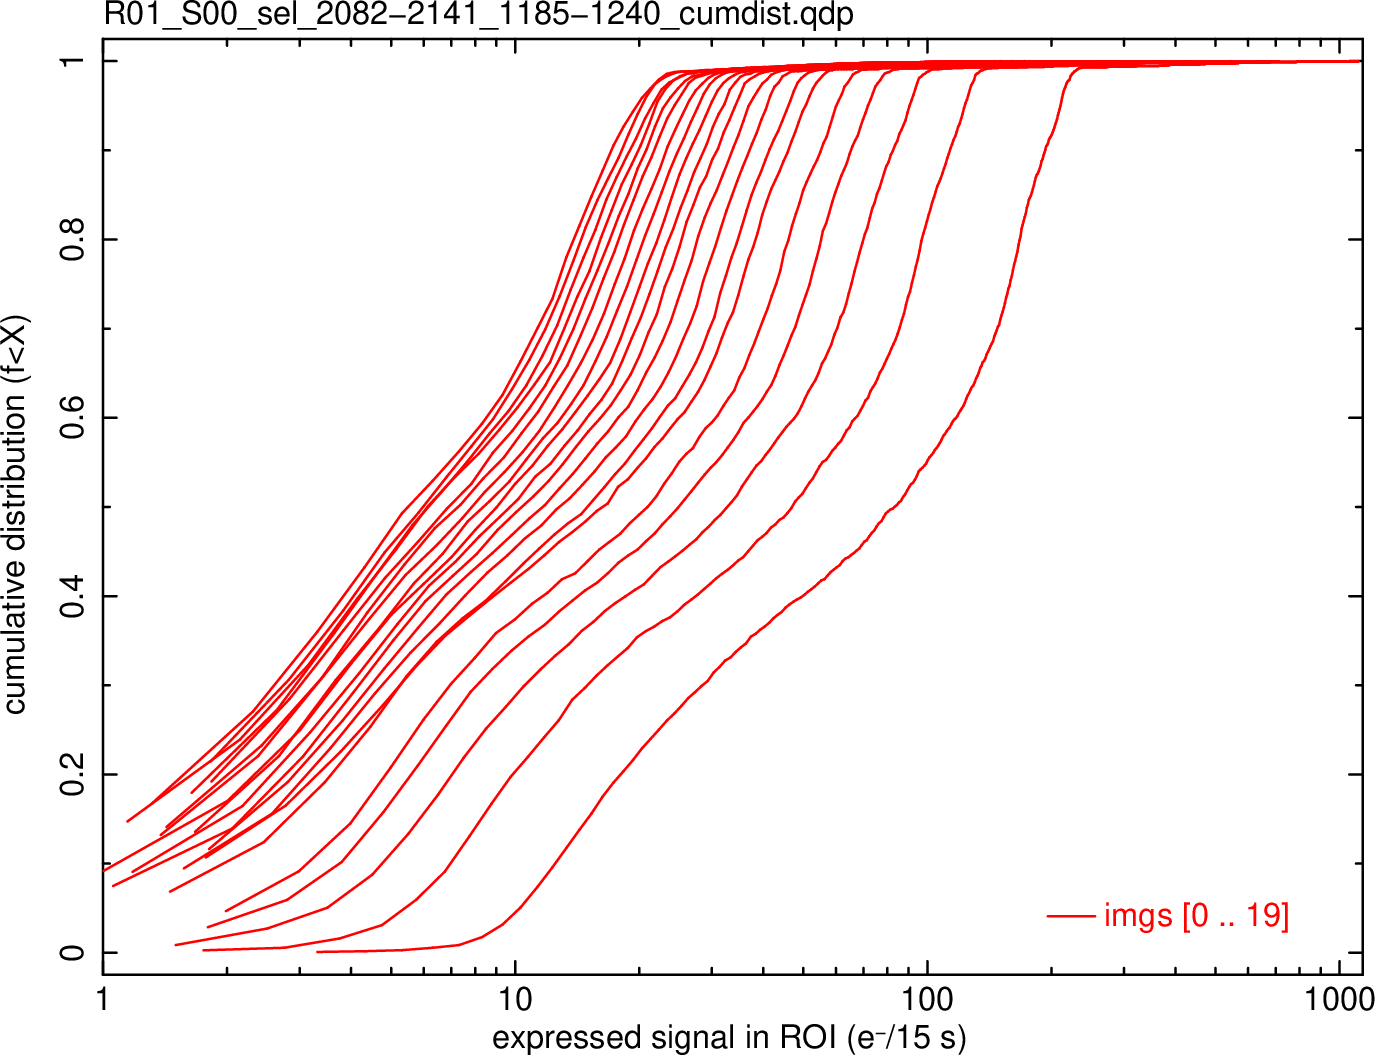
\includegraphics[width=\textwidth]{figures/phosphorescence-survey/phos_kinetics/R01_S00_sel_2082-2141_1185-1240_cumdist.png}    
\end{subfigure}
\hfil
\begin{subfigure}{0.45\textwidth}
  \centering
  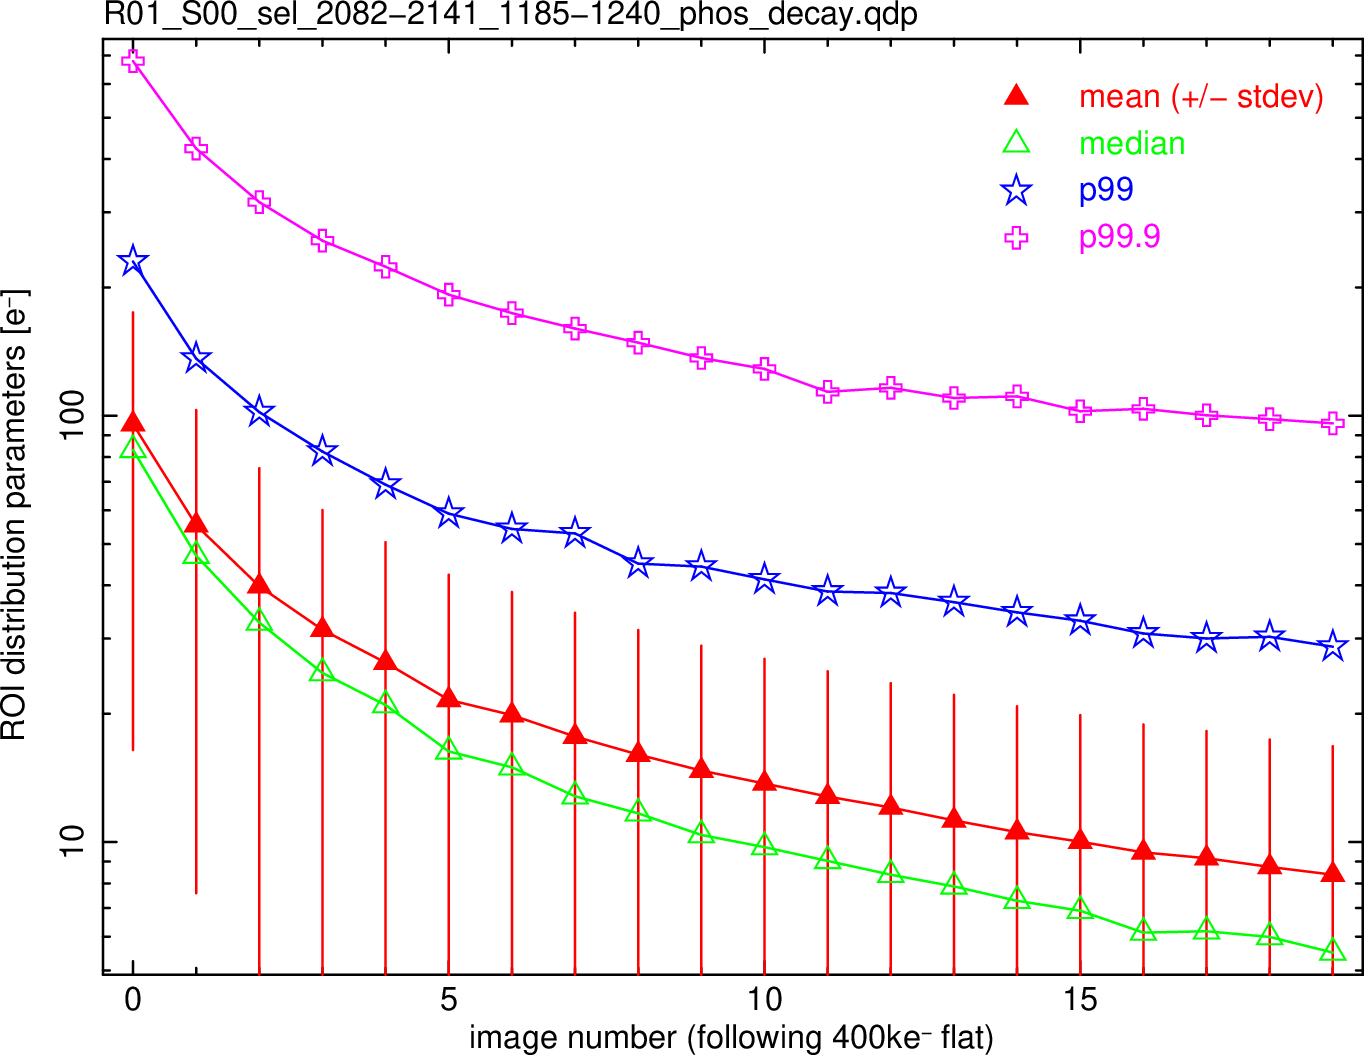
\includegraphics[width=\textwidth]{figures/phosphorescence-survey/phos_kinetics/R01_S00_sel_2082-2141_1185-1240_phos_decay.png}
\end{subfigure}
\newline
\caption{Kinetics for phosphorescence expression in ROIs of images for R01\_S00. This is the prominent cosmetic seen in Fig.~\ref{fig:phos:stains:R01S00}, which is apparently a {\it vampire} pixel.}
\label{fig:phos:kinetics:R01S00}
\end{figure}

\begin{figure}[!htbp]
\begin{subfigure}{0.45\textwidth}    
  \centering
  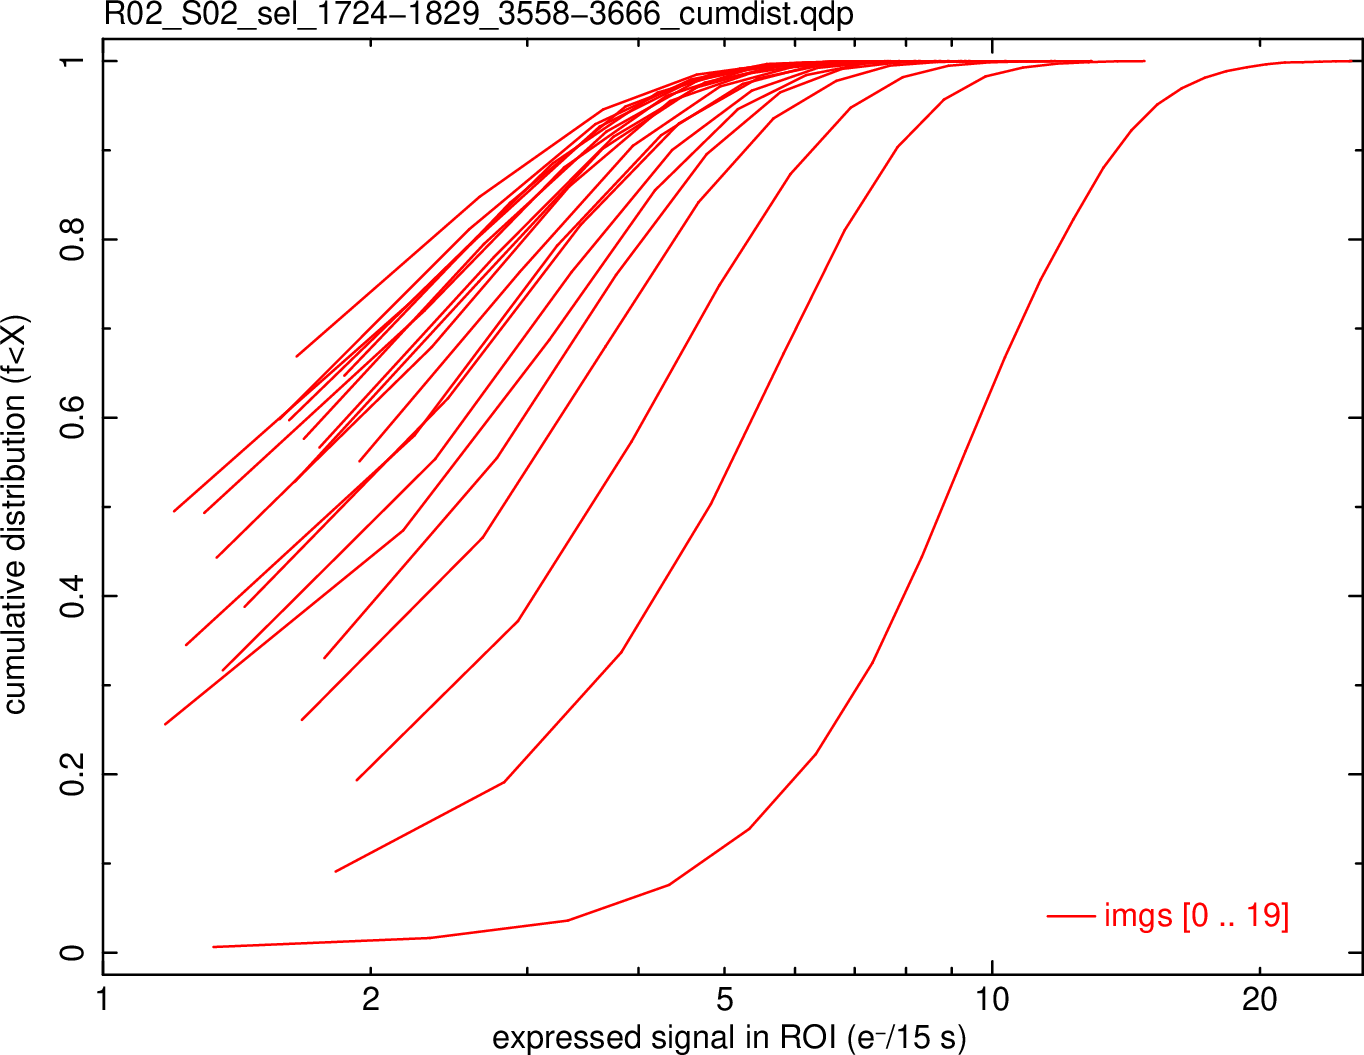
\includegraphics[width=\textwidth]{figures/phosphorescence-survey/phos_kinetics/R02_S02_sel_1724-1829_3558-3666_cumdist.png}    
\end{subfigure}
\hfil
\begin{subfigure}{0.45\textwidth}
  \centering
  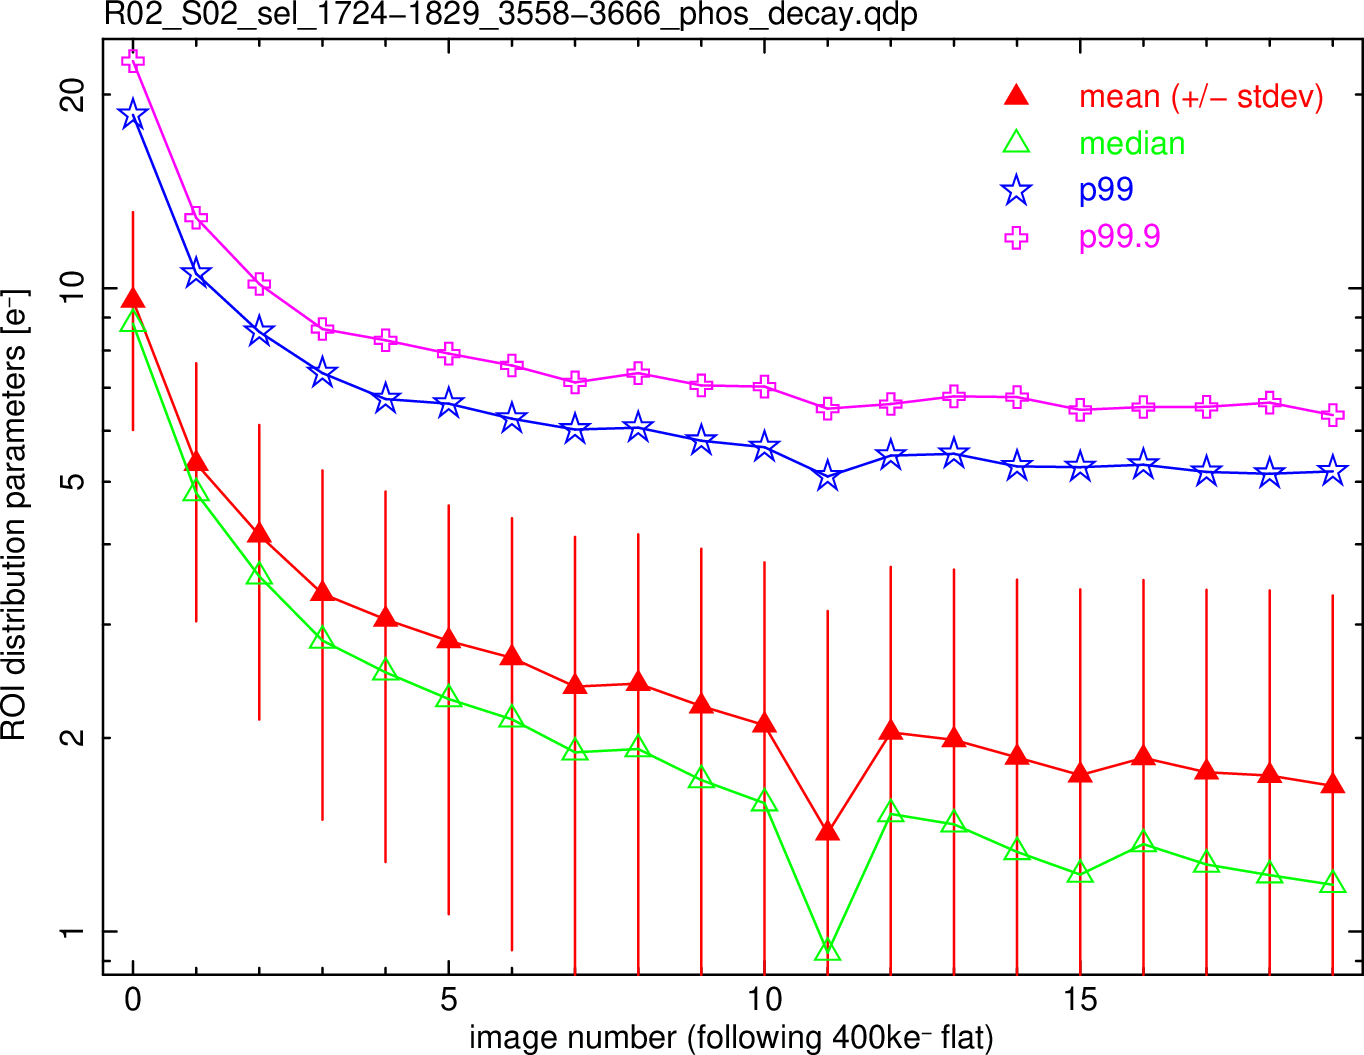
\includegraphics[width=\textwidth]{figures/phosphorescence-survey/phos_kinetics/R02_S02_sel_1724-1829_3558-3666_phos_decay.png}
\end{subfigure}
\newline
\begin{subfigure}{0.45\textwidth}    
  \centering
  \includegraphics[width=\textwidth]{figures/phosphorescence-survey/phos_kinetics/R02_S02_sel_1774-1880_3791-3900_cumdist.png}    
\end{subfigure}
\hfil
\begin{subfigure}{0.45\textwidth}
  \centering
  \includegraphics[width=\textwidth]{figures/phosphorescence-survey/phos_kinetics/R02_S02_sel_1774-1880_3791-3900_phos_decay.png}
\end{subfigure}
\newline
\begin{subfigure}{0.45\textwidth}    
  \centering
  \includegraphics[width=\textwidth]{figures/phosphorescence-survey/phos_kinetics/R02_S02_sel_2100-2206_3851-3959_cumdist.png}    
\end{subfigure}
\hfil
\begin{subfigure}{0.45\textwidth}
  \centering
  \includegraphics[width=\textwidth]{figures/phosphorescence-survey/phos_kinetics/R02_S02_sel_2100-2206_3851-3959_phos_decay.png}
\end{subfigure}
\newline
\caption{Kinetics for phosphorescence expression in ROIs of images for R02\_S02. This is the diffuse phosphorescence that correlates with the coffee stains seen in Fig.~\ref{fig:phos:stains:R02S02}. No extraction was performed on the {\it vampire pixel} found on the same sensor (R02\_S02\_C07).}
\label{fig:phos:kinetics:R02S02}
\end{figure}

\begin{figure}[!htbp]
\begin{subfigure}{0.45\textwidth}    
  \centering
  \includegraphics[width=\textwidth]{figures/phosphorescence-survey/phos_kinetics/R02_S12_sel_2556-2578_3445-3469_cumdist.png}    
\end{subfigure}
\hfil
\begin{subfigure}{0.45\textwidth}
  \centering
  \includegraphics[width=\textwidth]{figures/phosphorescence-survey/phos_kinetics/R02_S12_sel_2556-2578_3445-3469_phos_decay.png}
\end{subfigure}
\newline
\begin{subfigure}{0.45\textwidth}    
  \centering
  \includegraphics[width=\textwidth]{figures/phosphorescence-survey/phos_kinetics/R02_S12_sel_2695-2859_3353-3524_cumdist.png}    
\end{subfigure}
\hfil
\begin{subfigure}{0.45\textwidth}
  \centering
  \includegraphics[width=\textwidth]{figures/phosphorescence-survey/phos_kinetics/R02_S12_sel_2695-2859_3353-3524_phos_decay.png}
\end{subfigure}
\newline
\begin{subfigure}{0.45\textwidth}    
  \centering
  \includegraphics[width=\textwidth]{figures/phosphorescence-survey/phos_kinetics/R02_S12_sel_523-676_9-129_cumdist.png}    
\end{subfigure}
\hfil
\begin{subfigure}{0.45\textwidth}
  \centering
  \includegraphics[width=\textwidth]{figures/phosphorescence-survey/phos_kinetics/R02_S12_sel_523-676_9-129_phos_decay.png}
\end{subfigure}
\newline
\caption{Kinetics for phosphorescence expression in ROIs of images for R02\_S12. This is the structured phosphorescence that correlates with the coffee stains seen in Fig.~\ref{fig:phos:stains:R02S12}.}
\label{fig:phos:kinetics:R02S12}
\end{figure}

\begin{figure}[!htbp]
\begin{subfigure}{0.45\textwidth}    
  \centering
  \includegraphics[width=\textwidth]{figures/phosphorescence-survey/phos_kinetics/R03_S10_sel_2969-3010_1763-1800_cumdist.png}    
\end{subfigure}
\hfil
\begin{subfigure}{0.45\textwidth}
  \centering
  \includegraphics[width=\textwidth]{figures/phosphorescence-survey/phos_kinetics/R03_S10_sel_2969-3010_1763-1800_phos_decay.png}
\end{subfigure}
\newline
\begin{subfigure}{0.45\textwidth}    
  \centering
  \includegraphics[width=\textwidth]{figures/phosphorescence-survey/phos_kinetics/R03_S10_sel_2970-2985_1767-1797_cumdist.png}    
\end{subfigure}
\hfil
\begin{subfigure}{0.45\textwidth}
  \centering
  \includegraphics[width=\textwidth]{figures/phosphorescence-survey/phos_kinetics/R03_S10_sel_2970-2985_1767-1797_phos_decay.png}
\end{subfigure}
\newline
\begin{subfigure}{0.45\textwidth}    
  \centering
  \includegraphics[width=\textwidth]{figures/phosphorescence-survey/phos_kinetics/R03_S10_sel_2995-3009_1767-1797_cumdist.png}    
\end{subfigure}
\hfil
\begin{subfigure}{0.45\textwidth}
  \centering
  \includegraphics[width=\textwidth]{figures/phosphorescence-survey/phos_kinetics/R03_S10_sel_2995-3009_1767-1797_phos_decay.png}
\end{subfigure}
\newline
\caption{Kinetics for phosphorescence expression in ROIs of images for R03\_S10. These describe regions including or near the bright/focusing {\it vampire pixel} seen in Figs.~\ref{fig:phos:stains:R03S10}, \ref{subfig:phosresp_R03_S10} and \ref{subfig:hvb_on_R03_S10}.}
\label{fig:phos:kinetics:R03S10}
\end{figure}

\begin{figure}[!htbp]
\begin{subfigure}{0.45\textwidth}    
  \centering
  \includegraphics[width=\textwidth]{figures/phosphorescence-survey/phos_kinetics/R20_S20_sel_1820-1920_535-635_cumdist.png}    
\end{subfigure}
\hfil
\begin{subfigure}{0.45\textwidth}
  \centering
  \includegraphics[width=\textwidth]{figures/phosphorescence-survey/phos_kinetics/R20_S20_sel_1820-1920_535-635_phos_decay.png}
\end{subfigure}
\newline
\caption{Kinetics for phosphorescence expression in ROIs of images for R20\_S20. These describe the prominent non-focusing {\it vampire pixel} seen in Figs.~\ref{subfig:phosresp_R20_S20} and \ref{subfig:hvb_on_R20_S20}.}
\label{fig:phos:kinetics:R20S20}
\end{figure}

\begin{figure}[!htbp]
\begin{subfigure}{0.45\textwidth}    
  \centering
  \includegraphics[width=\textwidth]{figures/phosphorescence-survey/phos_kinetics/R43_S11_sel_1741-1955_3754-3806_cumdist.png}    
\end{subfigure}
\hfil
\begin{subfigure}{0.45\textwidth}
  \centering
  \includegraphics[width=\textwidth]{figures/phosphorescence-survey/phos_kinetics/R43_S11_sel_1741-1955_3754-3806_phos_decay.png}
\end{subfigure}
\newline
\begin{subfigure}{0.45\textwidth}    
  \centering
  \includegraphics[width=\textwidth]{figures/phosphorescence-survey/phos_kinetics/R43_S11_sel_1763-1976_3826-3878_cumdist.png}    
\end{subfigure}
\hfil
\begin{subfigure}{0.45\textwidth}
  \centering
  \includegraphics[width=\textwidth]{figures/phosphorescence-survey/phos_kinetics/R43_S11_sel_1763-1976_3826-3878_phos_decay.png}
\end{subfigure}
\newline
\begin{subfigure}{0.45\textwidth}    
  \centering
  \includegraphics[width=\textwidth]{figures/phosphorescence-survey/phos_kinetics/R43_S11_sel_40-90_2751-2957_cumdist.png}    
\end{subfigure}
\hfil
\begin{subfigure}{0.45\textwidth}
  \centering
  \includegraphics[width=\textwidth]{figures/phosphorescence-survey/phos_kinetics/R43_S11_sel_40-90_2751-2957_phos_decay.png}
\end{subfigure}
\newline
\caption{Kinetics for phosphorescence expression in ROIs of images for R43\_S11. These describe bright, diffuse transient regions seen in Figs.~\ref{fig:phos:stains:R43S11} and \ref{subfig:hvb_on_R43_S11}, which apparently turn off completely when the HV Bias is {\it off}.}
\label{fig:phos:kinetics:R43S11}
\end{figure}

\begin{figure}[!htbp]
\begin{subfigure}{0.45\textwidth}    
  \centering
  \includegraphics[width=\textwidth]{figures/phosphorescence-survey/phos_kinetics/R43_S20_sel_207-292_3352-3435_cumdist.png}    
\end{subfigure}
\hfil
\begin{subfigure}{0.45\textwidth}
  \centering
  \includegraphics[width=\textwidth]{figures/phosphorescence-survey/phos_kinetics/R43_S20_sel_207-292_3352-3435_phos_decay.png}
\end{subfigure}
\newline
\begin{subfigure}{0.45\textwidth}    
  \centering
  \includegraphics[width=\textwidth]{figures/phosphorescence-survey/phos_kinetics/R43_S20_sel_547-633_3346-3430_cumdist.png}    
\end{subfigure}
\hfil
\begin{subfigure}{0.45\textwidth}
  \centering
  \includegraphics[width=\textwidth]{figures/phosphorescence-survey/phos_kinetics/R43_S20_sel_547-633_3346-3430_phos_decay.png}
\end{subfigure}
\newline
\begin{subfigure}{0.45\textwidth}    
  \centering
  \includegraphics[width=\textwidth]{figures/phosphorescence-survey/phos_kinetics/R43_S20_sel_707-816_3373-3589_cumdist.png}    
\end{subfigure}
\hfil
\begin{subfigure}{0.45\textwidth}
  \centering
  \includegraphics[width=\textwidth]{figures/phosphorescence-survey/phos_kinetics/R43_S20_sel_707-816_3373-3589_phos_decay.png}
\end{subfigure}
\newline
\caption{Kinetics for phosphorescence expression in ROIs of images for R43\_S20. These include some of the the highly structured {\it snowflake-like} transient regions seen in Figs.~\ref{subfig:hvb_on_R43_S20} and \ref{fig:phos:stains:R43S20}.}
\label{fig:phos:kinetics:R43S20}
\end{figure}

\clearpage
\section{Phosphorescence response characterization}
\label{sect:response}
Figures~\ref{fig:phos:resp:R01S00} through \ref{fig:phos:resp:R43S20} attempt to quantify the expressed phosphorescence response in ROIs on seven of the problematic ITL sensors. Previously, we had captured the phosphorescence {\it transient term} across the ITL sensors ({\it cf.} Figs.~\ref{fig:phos:R00} thru \ref{fig:phos:R44}); we also tracked ROI pixel distribution parameters of individual median images constructed from the selection of specific images acquired across the 20 B-protocol datasets available (listed in Table~\ref{tab:phosphorescence:datasets}). Here we analyze the signal level- and wavelength-dependences of the expressed phosphorescence captured in the first dark image following flat exposure. Table~XX provides the image numbers.. 

Because these runs were performed to sample a two dimensional parameter space,  that would lead to 

By fitting decay models to these persistence curves, it is immediately clear that there are multiple (>2) timescales at play for the pixels in each ROI. An example of such a fit is given in Figure~\ref{fig:phos:kinetics:fit:R20S20C13} where a 3-population relaxation model is used to characterize evolution of the 99\% quantile level of the distribution. In this case, there are three different exponential timescales determined: $(\tau_1,\tau_2,\tau_3) = (0.62,2.5,18.3)$ in image units (10.9, 43.8 \& 320 seconds, respectively). The corresponding ratio of these populations works out to 4.5\% (fast), 21.5\% (medium) and 74\% (slow), respectively. Inspection of the more detailed parameters plotted generally indicate skewed distributions from mismatches between medians and means; the choice of the 99\% quantile level to characterize was mainly to estimate the degree to which images would need to be phosphorescence-corrected (and/or the variance plane modified, given the asymmetric impact of the position specific, phosphorescence contribution in recorded images). 

%\begin{figure}[!htbp]
%\centering
%\begin{subfigure}{0.8\textwidth}    
%  \centering
%  \includegraphics[width=\textwidth]{figures/phosphorescence-%survey/phos_kinetics/R20_S20_sel_1820-1920_535-635_phos_decay_fit.png}    
%\end{subfigure}
%\caption{A three-population fit of the phosphorescence expressed by the %vapire pixel region of R20\_S20\_C13. The fit was performed on the 99\% %quantile level where signal levels are well above the $3\sigma$ level of %the noise distribution. Here, image numbers are parasitically used as %time units, with roughly 17.5 seconds per image.}
%\label{fig:phos:resp:fit:R20S20C13}
%\end{figure}

\begin{figure}[!htbp]
\centering
\begin{subfigure}{0.45\textwidth}    
  \centering
  \includegraphics[width=\textwidth]{figures/phosphorescence-survey/phos_resp/resp_99_R01_S00_1961-2020_1268-1325.png}    
\end{subfigure}
\newline
\centering
\begin{subfigure}{0.45\textwidth}    
  \centering
  \includegraphics[width=\textwidth]{figures/phosphorescence-survey/phos_resp/resp_99_R01_S00_1983-2042_1065-1121.png}    
\end{subfigure}
\newline
\centering
\begin{subfigure}{0.45\textwidth}    
  \centering
  \includegraphics[width=\textwidth]{figures/phosphorescence-survey/phos_resp/resp_99_R01_S00_2082-2141_1185-1240.png}    
\end{subfigure}
\newline
\caption{Signal and wavelength response for phosphorescence expression (99\% level) in ROIs of images for R01\_S00. This is the prominent cosmetic seen in Fig.~\ref{fig:phos:stains:R01S00}, which is apparently a {\it vampire} pixel.}
\label{fig:phos:resp:R01S00}
\end{figure}

\begin{figure}[!htbp]
\centering
\begin{subfigure}{0.45\textwidth}    
  \centering
  \includegraphics[width=\textwidth]{figures/phosphorescence-survey/phos_resp/resp_99_R02_S02_1724-1829_3558-3666.png}    
\end{subfigure}
\newline
\centering
\begin{subfigure}{0.45\textwidth}    
  \centering
  \includegraphics[width=\textwidth]{figures/phosphorescence-survey/phos_resp/resp_99_R02_S02_1774-1880_3791-3900.png}    
\end{subfigure}
\newline
\centering
\begin{subfigure}{0.45\textwidth}    
  \centering
  \includegraphics[width=\textwidth]{figures/phosphorescence-survey/phos_resp/resp_99_R02_S02_2100-2206_3851-3959.png}    
\end{subfigure}
\newline
\caption{Signal and wavelength response for phosphorescence expression (99\% level) in ROIs of images for R02\_S02. This is the diffuse phosphorescence that correlates with the coffee stains seen in Fig.~\ref{fig:phos:stains:R02S02}. No extractions were performed on the {\it vampire pixels} found on the same sensor (R02\_S02\_C15 and R02\_S02\_C07).}
\label{fig:phos:resp:R02S02}
\end{figure}

\begin{figure}[!htbp]
\centering
\begin{subfigure}{0.45\textwidth}    
  \centering
  \includegraphics[width=\textwidth]{figures/phosphorescence-survey/phos_resp/resp_99_R02_S12_2556-2578_3445-3469.png}    
\end{subfigure}
\newline
\centering
\begin{subfigure}{0.45\textwidth}    
  \centering
  \includegraphics[width=\textwidth]{figures/phosphorescence-survey/phos_resp/resp_99_R02_S12_2695-2859_3353-3524.png}    
\end{subfigure}
\newline
\centering
\begin{subfigure}{0.45\textwidth}    
  \centering
  \includegraphics[width=\textwidth]{figures/phosphorescence-survey/phos_resp/resp_99_R02_S12_523-676_9-129.png}    
\end{subfigure}
\newline
\caption{Signal and wavelength response for phosphorescence expression (99\% level) in ROIs of images for R02\_S12. This is the structured phosphorescence that correlates with the coffee stains seen in Fig.~\ref{fig:phos:stains:R02S12}.}
\label{fig:phos:resp:R02S12}
\end{figure}

\begin{figure}[!htbp]
\centering
\begin{subfigure}{0.45\textwidth}    
  \centering
  \includegraphics[width=\textwidth]{figures/phosphorescence-survey/phos_resp/resp_99_R03_S10_2969-3010_1763-1800.png}    
\end{subfigure}
\newline
\centering
\begin{subfigure}{0.45\textwidth}    
  \centering
  \includegraphics[width=\textwidth]{figures/phosphorescence-survey/phos_resp/resp_99_R03_S10_2970-2985_1767-1797.png}    
\end{subfigure}
\newline
\centering
\begin{subfigure}{0.45\textwidth}    
  \centering
  \includegraphics[width=\textwidth]{figures/phosphorescence-survey/phos_resp/resp_99_R03_S10_2995-3009_1767-1797.png}    
\end{subfigure}
\newline
\caption{Signal and wavelength response for phosphorescence expression (99\% level) in ROIs of images for R03\_S10. These describe regions including or near the bright/focusing {\it vampire pixel} seen in Figs.~\ref{fig:phos:stains:R03S10}, \ref{subfig:phosresp_R03_S10} and \ref{subfig:hvb_on_R03_S10}.}
\label{fig:phos:resp:R03S10}
\end{figure}

\begin{figure}[!htbp]
\centering
\begin{subfigure}{0.45\textwidth}    
  \centering
  \includegraphics[width=\textwidth]{figures/phosphorescence-survey/phos_resp/resp_99_R20_S20_1820-1920_535-635.png}    
\end{subfigure}
\newline
\caption{Signal and wavelength response for phosphorescence expression (99\% level) in an ROI of images for R20\_S20. These describe the prominent non-focusing {\it vampire pixel} seen in Figs.~\ref{subfig:phosresp_R20_S20} and \ref{subfig:hvb_on_R20_S20}.}
\label{fig:phos:kinetics:R20S20}
\end{figure}

\begin{figure}[!htbp]
\centering
\begin{subfigure}{0.45\textwidth}    
  \centering
  \includegraphics[width=\textwidth]{figures/phosphorescence-survey/phos_resp/resp_99_R43_S11_1741-1955_3754-3806.png}    
\end{subfigure}
\newline
\centering
\begin{subfigure}{0.45\textwidth}    
  \centering
  \includegraphics[width=\textwidth]{figures/phosphorescence-survey/phos_resp/resp_99_R43_S11_1763-1976_3826-3878.png}    
\end{subfigure}
\newline
\centering
\begin{subfigure}{0.45\textwidth}    
  \centering
  \includegraphics[width=\textwidth]{figures/phosphorescence-survey/phos_resp/resp_99_R43_S11_40-90_2751-2957.png}    
\end{subfigure}
\newline
\caption{Signal and wavelength response for phosphorescence expression (99\% level) in ROIs of images for R43\_S11. These describe bright, diffuse transient regions seen in Figs.~\ref{fig:phos:stains:R43S11} and \ref{subfig:hvb_on_R43_S11}, which apparently turn off completely when the HV Bias is {\it off}.}
\label{fig:phos:resp:R43S11}
\end{figure}

\begin{figure}[!htbp]
\centering
\begin{subfigure}{0.45\textwidth}    
  \centering
  \includegraphics[width=\textwidth]{figures/phosphorescence-survey/phos_resp/resp_99_R43_S20_207-292_3352-3435.png}    
\end{subfigure}
\newline
\centering
\begin{subfigure}{0.45\textwidth}    
  \centering
  \includegraphics[width=\textwidth]{figures/phosphorescence-survey/phos_resp/resp_99_R43_S20_547-633_3346-3430.png}    
\end{subfigure}
\newline
\centering
\begin{subfigure}{0.45\textwidth}    
  \centering
  \includegraphics[width=\textwidth]{figures/phosphorescence-survey/phos_resp/resp_99_R43_S20_707-816_3373-3589.png}    
\end{subfigure}
\newline
\caption{Signal and wavelength response for phosphorescence expression (99\% level) in ROIs of images for R43\_S20. These include some of the the highly structured {\it snowflake-like} transient regions seen in Figs.~\ref{subfig:hvb_on_R43_S20} and \ref{fig:phos:stains:R43S20}.}
\label{fig:phos:resp:R43S20}
\end{figure}

\clearpage
